\documentclass[openright,twoside,12pt]{book}

\usepackage[a4paper,left=2cm,top=2.5cm,right=1.5cm,bottom=2.5cm]{geometry}
\usepackage{times}
\usepackage{array}
\usepackage[spanish,es-lcroman]{babel} % espanol
\usepackage[utf8]{inputenc} % acentos sin codigo
\usepackage{graphicx} % gráficos
\usepackage{lscape}
\usepackage{hyperref}
\usepackage{fancyvrb}
%\usepackage{fancyhdr}
\usepackage{wrapfig}
\setlength{\parskip}{10pt}
\usepackage{titlesec}
\usepackage{eurosym}
\usepackage{colortbl}
\usepackage{xcolor}
\usepackage{listingsutf8}
\usepackage{float}
\usepackage{chngcntr}
\usepackage{dirtree}
\usepackage{url}
\usepackage{booktabs}
  
\addtolength{\headsep}{4mm}

%\counterwithout{figure}{chapter}
%\counterwithout{table}{chapter}

%%%%%%%%%%%%%%%%%%%
% Cosas de Listings
%%
\lstdefinelanguage{json}{
    basicstyle=\normalfont\ttfamily,
    numbersep=8pt,
    showstringspaces=false,
    breaklines=true,
    frame=lines,
    backgroundcolor=\color{white}
}

\lstdefinestyle{codigoerlang}{
  basickstyle=\sffamily\small,
}

\lstdefinestyle{terminal}{
  basicstyle=\ttfamily\small, % Set the basic font style
  backgroundcolor=\color{lightgray}, % Set the background color
  keywordstyle=\color{white}, % Set keyword color
  stringstyle=\color{yellow}, % Set string color
  frame=single, % Add a frame around the code listing
  breaklines=true, % Enable line breaking
  showstringspaces=false % Don't show spaces in strings as a special character
}

\renewcommand{\lstlistingname}{Listado} % en castellano
%% Fin de cosas de Listings

\frontmatter
\pagenumbering{roman} 

\date{Julio de 2023}
\author{Martín Tornero Vázquez}

\title{Aplicación de Adquisición de Datos de Sensores Mediante 
Raspberry-pi en \strut{}Entorno Erlang}

\begin{document}

\begin{titlepage}

\begin{center}
\vspace*{-2cm}
\begin{figure}[htb]
\begin{center}

\includegraphics[width=5cm]{images/escudo_uva.png}
\end{center}
\end{figure}
\begin{large}
\textbf{Universidad de Valladolid}
\end{large}

\vspace*{1cm}

\begin{large}
\textbf{ESCUELA DE INGENIERÍA INFORMÁTICA DE VALLADOLID}

\end{large}
\vspace*{0.5cm}
{\sc \textbf{ Grado en Ingeniería Informática}\\
	\textbf{Mención en Tecnologías de la Información}}

\vspace*{1.5cm}
\rule{\textwidth}{0.1mm}
{\huge\sc Aplicación de Adquisición de Datos de\strut\\
          Sensores Mediante Raspberry-Pi en\strut\\
          Entorno Erlang OTP}
\vspace*{1cm}
\rule{\textwidth}{0.1mm}\\
\vspace*{3cm}
\begin{large}
\begin{flushright}
Alumno:\\
\textbf{Martín Tornero Vázquez}

\vspace*{0.3in}
Tutor:\\
\textbf{Dr. César Llamas Bello}%
	%\newline \textbf{Dr. Otrez Profesorez Profesorez} % si hay más de uno
\end{flushright}
\end{large}
\end{center}

\end{titlepage}
\cleardoublepage


\thispagestyle{empty}

\vspace*{12cm}

\begin{minipage}{12cm}
\large
Este documento describe la memoria del Trabajo de Fin de Grado realizado por D. Martín Tornero Vázquez bajo la supervisión del profesor Dr. César Llamas Bello, para la obtención del Título de Ingeniero en Informática en la Mención de Tecnologías de la Información en la Escuela de Ingeniería Informática de Valladolid, en julio de 2023. 

\ \newline



\ \newline


En Valladolid, a fecha de firma electrónica

\ \newline


\emph{Martín Tornero Vázquez}
\end{minipage}

\newpage
\chapter*{Resumen}
\addcontentsline{toc}{chapter}{Resumen}
\begin{center}
    \begin{minipage}[h]{0.8\textwidth}

Este Trabajo de Fin de Grado describe la implementación de una plataforma de sensorización basada en Raspberry-Pi y el lenguaje de programación Erlang OTP, bajo la forma de un servicio Web que permite la toma de datos. Bajo esta premisa, esta plataforma y aplicación nos permite  permite evaluar la dificultad de la construcción de un sistema de este tipo y las prestaciones que puede ofrecer.\\

Erlang OTP es una plataforma ampliamente utilizada en entornos de alta disponibilidad, pero su utilización como lenguaje de construcción de sistemas de IoT no es tan amplia por las dificultades que conlleva la interacción con otros lenguajes y sus necesidades de memoria y cómputo. En este proyecto hemos comprobado la relativa facilidad con la que podemos construir este tipo de sistemas y las prestaciones que ofrece.

\parskip 1cm

\textbf{Palabras clave}: Erlang OTP, C, Raspberry-Pi, Sensores, IoT.
  \end{minipage}
\end{center}


\chapter*{Abstract}
\addcontentsline{toc}{chapter}{Abstract}
\begin{center}
    \begin{minipage}[h]{0.8\textwidth}


This Final Degree Project describes the implementation of a sensorization platform based on Raspberry-Pi and the Erlang OTP programming language, which provides a web service for data collection and serves to evaluate the difficulties involved in interacting with other languages and its requirements. Under this premise, this platform and application permits to evaluate the difficulty of building a system of this kind and the features it can offer.

Erlang OTP is a widely used platform in high availability environments, but its use as a language for building IoT systems is not as extensive due to the difficulties involved in interacting with other languages and its memory and computation requirements. In this project, we have verified the relative ease with which we can build this type of system and the features it provides.

\parskip 1cm

\textbf{Keywords}: Erlang OTP, C, Raspberry-Pi, Sensors, IoT.
\end{minipage}
\end{center}


\tableofcontents

\addcontentsline{toc}{chapter}{Lista de figuras} % para que aparezca en el indice de contenidos
\listoffigures % indice de figuras

\cleardoublepage

\addcontentsline{toc}{chapter}{Lista de tablas} % para que aparezca en el indice de contenidos
\listoftables % indice de tablas

\cleardoublepage
\addcontentsline{toc}{chapter}{Lista de listados} % indice de listados

\lstlistoflistings

\mainmatter


\nocite{*}


\chapter{Presentación}\label{cap.introduccion}

\section{Objetivo}%
\label{sec:Objetivo}

El objetivo de este proyecto es construir y documentar una plataforma funcional que permita la recogida de datos de sensores mediante una interfaz web sobre Hardware Raspberry-Pi mediante el lenguaje Erlang OTP, en lo sucesivo abreviaremos por <<Erlang>> (como la función de distribución de probabilidad).

El objetivo principal es obtener un prototipo final funcional que permita recoger los datos y analizarlos, sin embargo, el objetivo global del trabajo será analizar la diferencia entre los distintos sensores, protocolos y lenguajes a utilizar, ver su viabilidad, la complejidad que conlleva y obtener conclusiones razonadas sobre la utilización de Erlang para este uso.


\section{Motivación}

La domotización de los hogares y las empresas está cada vez mas en auge y por tanto mas solicitada a los técnicos informáticos.

El uso de sensores ofrece una amplia gama de beneficios para las empresas en la actualidad. Su implementación estratégica puede impulsar el crecimiento, mejorar la eficiencia operativa y brindar una ventaja competitiva significativa. Entre algunos de los beneficios que aporta el uso de este tipo de herramientas encontramos: La optimización de procesos, el mantenimiento predictivo, la posible mejora de la seguridad y la toma de decisiones basada en datos precisos.

A pesar de la existencia de proyectos similares utilizando otras tecnologías, este trabajo trata de analizar el uso del lenguaje Erlang para crear servidores que permitan leer y analizar los datos obtenidos de los sensores dispuestos en un marco empresarial o doméstico y si se trata de una elección sólida para el desarrollo de este tipo de servidores. Sobre el papel, las características únicas de Erlang lo convierten en un lenguaje altamente eficiente y confiable para este tipo de aplicaciones ya que entre otras, una de las fortalezas clave de este lenguaje es su capacidad para manejar la concurrencia y la escalabilidad. Un servidor Erlang puede gestionar de manera eficiente múltiples solicitudes simultáneas provenientes de diferentes sensores distribuidos en una red.

El modelo de concurrencia de Erlang, basado en actores y en el intercambio de mensajes ligero, permite un manejo eficiente de la concurrencia sin preocuparse por los problemas habituales como las condiciones de carrera o los bloqueos. A mayores, Erlang es ampliamente conocido por su sistema de tolerancia a fallos integrado, sobretodo en servidores, lo que es fundamental cuando se trata de aplicaciones críticas como el monitoreo de sensores en un entorno empresarial.

\section{Propósito general}

El propósito global es conseguir un servidor Erlang operativo que permita conocer la información de los sensores conectados a la placa R-Pi, a través del cual se puedan lanzar la lectura de los mismos y obtener los datos obtenidos para su análisis. Para ello se implementará:

\begin{itemize}

    \item Una placa Raspberry-Pi3 con sistema operativo Raspbian que dispondrá de los sensores conectados a sus pines GPIO.
    
    \item Los programas C que ejecuten los sensores y almacenen sus datos en archivos de texto.
    
    \item Un servidor creado mediante Erlang con una sencilla interfaz web usando HTML y JSON.
    
    \item Diseño de un API REST HTTP robusta que permita el empleo de los sensores desde un terminal usando el mínimo de recursos.
\end{itemize}

En cómputo, se implementará una aplicación Erlang OTP que modele la lógica del servidor, esta aplicación hará uso de un servidor Web Cowboy y los códigos C que permitan la ejecución y lectura de datos de los sensores.

\section{Entorno tecnológico}

En el proyecto se utilizan distintas tecnologías hardware y software que tienen que ver con tres áreas de desarrollo distintas, como son la del desarrollo del servidor asociado a los sensores, la tecnología de desarrollo del cliente y finalmente aquellas propias del hardware de Rasoberry-Pi. A continuación se desglosa por cada una de las cuales son los elementos tecnológicos más relevantes:

\begin{itemize}
 \item Tecnologías de Servidor:
 \begin{itemize}
     \item Aplicación Erlang OTP: Responsable del correcto funcionamiento del servidor; inicialización, finalización y conexiones.
     \item Servidor Web Cowboy: Responsable de la trasmisión de información entre el servidor y la placa R-Pi, así como la visualización web.
 \end{itemize}
 
\item \textbf{Cliente:}
\begin{itemize}
    \item JSON: Responsable de almacenar todas las descripciones de los usuarios y el manual de uso
\end{itemize}

\item \textbf{Raspberry-Pi:}
\begin{itemize}
    \item Códigos C: Programación de los diferentes sensores para obtener datos y almacenarlos en un archivo, serán invocados por el servidor.
\end{itemize}
\end{itemize}


\section{Organización de la memoria}

La documentación ha sido estructurada de la siguiente forma:

En primer lugar, se ha realizado una presentación de los conceptos básicos sobre el proyecto en la cual se enumeran y describen cada uno de los componentes hardware del mismo así como herramientas software utilizadas y lenguajes de programación usados.

El proyecto se ha dividido en tres prototipos:
\begin{itemize}
    \item Prototipo de Exploración: Se describe el desarrollo inicial del sistema, la configuración de la Rasperry-Pi así como la conexión de los sensores y su implementación.
    \item Prototipo Incremental: Se describe como puede utilizarse Erlang sobre Raspberry-Pi 3 así como diferentes métodos de instalación de este lenguaje sobre esta.
    \item Prototipo funcional: Se explica como se ha creado el servidor y cada una de sus partes y se describen las pruebas realizadas sobre el mismo.
\end{itemize}

Por último, encontramos las conclusiones obtenidas del proyecto y las posibilidades de ampliación del mismo.



\chapter{Contexto tecnológico}

En este apartado se describirá, de manera sencilla, diversas tecnologías que se utilizarán en el proyecto, bien porque forman parte de las restricciones de nuestra solución, o bien como consecuencia de decisiones tomadas en la elaboración de los prototipos que forman parte del desarrollo del trabajo.
Este contexto incluye hardware como la propia Raspberrhy Pi, una plataforma de S.O. y lenguajes y bibliotecas de programación como C, Erlang OTP o el módulo Cowboy.


\section{Erlang OTP}

Erlang OTP es un lenguaje de programación diseñado para sistemas distribuidos y concurrentes. Fue desarrollado por Ericsson, una compañía sueca de telecomunicaciones, en los años 80 para programar sistemas de telecomunicaciones, pero desde entonces ha sido utilizado en una amplia variedad de aplicaciones, desde servidores web hasta sistemas de control de procesos industriales. Erlang toma su nombre de Agner Erlang, un matemático danés que desarrolló la teoría de colas, que es fundamental en el diseño de sistemas de telecomunicaciones.

Erlang se puede considerar como un lenguaje híbrido, ya que combina elementos funcionales, imperativos y algunos aspectos de la programación orientada a objetos, aunque no de manera completa. Sin embargo, su principal fortaleza radica en ser un lenguaje orientado a la concurrencia. Ofrece una gran capacidad para desarrollar sistemas distribuidos, paralelos y concurrentes, y proporciona mecanismos para manejar la tolerancia a fallos de manera efectiva.

Desde sus inicios, Erlang fue diseñado para ejecutarse de forma continua, lo que significa que se pueden realizar cambios en el código de las aplicaciones sin necesidad de detener su ejecución. Esto permite una alta disponibilidad y actualizaciones sin interrupciones.
\newpage
\subsection{Características Principales}

A continuación, se enumerarán las principales características de Erlang:

\begin{enumerate}
    \item \textbf{Concurrencia}: Erlang está diseñado para manejar la concurrencia y la ejecución paralela de forma eficiente. El modelo de concurrencia se basa en la ejecución simultánea de procesos ligeros (actores) que se comunican a través del intercambio de mensajes.
    \item \textbf{Tolerancia a fallos}: Los sistemas desarrollados en Erlang pueden recuperarse automáticamente de errores sin perder la integridad de los datos o la funcionalidad general del sistema. Esto se logra mediante la supervisión de procesos, la capacidad de reiniciar procesos y la capacidad de detectar y responder a excepciones.
    \item \textbf{Escalabilidad}: Erlang se adapta bien a sistemas escalables debido a su modelo de concurrencia ligera y su capacidad para distribuir procesos en múltiples nodos. 
    \item \textbf{Hot swapping}:  Erlang permite la actualización en caliente de código y módulos en tiempo de ejecución sin interrumpir la ejecución del sistema. Esto es especialmente útil para sistemas en funcionamiento continuo que no pueden permitirse detenerse para actualizaciones.
    \item \textbf{Programación funcional}: Erlang es un lenguaje funcional puro, lo que significa que se basa en la evaluación de expresiones y la inmutabilidad de los datos. Esto promueve un estilo de programación declarativo, utilizando asignaciones únicas lo cual reduce los efectos secundarios y facilita el razonamiento sobre el código así como mejora la capacidad de prueba y depuración.
\end{enumerate}

\subsection{Erlang en la actualidad}

En la actualidad, Erlang sigue siendo un lenguaje de programación relevante y utilizado en diversos ámbitos, entre otros:

\begin{itemize}

    \item \textbf{Telecomunicaciones}: Especialmente en sistemas de conmutación telefónica y en aplicaciones de redes de telecomunicaciones.
    
    \item \textbf{Aplicaciones en tiempo real}:  Sistemas de mensajería instantánea, plataformas de juegos en línea y sistemas de transmisión de datos en tiempo real. Su modelo de concurrencia basado en actores y su capacidad para manejar grandes volúmenes de transacciones en paralelo lo hacen muy adecuado para este tipo de aplicaciones.
    
    \item \textbf{Sistemas distribuidos y escalables}: Su capacidad para distribuir procesos en múltiples nodos y su enfoque en la programación concurrente lo convierten en una herramienta poderosa para construir sistemas que pueden crecer y adaptarse a medida que aumentan los requisitos de rendimiento.
    
    \item \textbf{Internet de las cosas (IoT)}: Erlang se ha utilizado cada vez más en el ámbito del IoT, ya que su enfoque en la concurrencia y la escalabilidad lo hace adecuado para gestionar grandes cantidades de dispositivos conectados. Su capacidad para manejar eventos y su tolerancia a fallos también son beneficiosos en entornos IoT donde la fiabilidad y la capacidad de respuesta son fundamentales.
    
    \item \textbf{Sistemas críticos}:  Erlang ha demostrado ser un lenguaje robusto y confiable para el desarrollo de sistemas críticos en los que la tolerancia a fallos y la disponibilidad continua son esenciales. Esto incluye aplicaciones en sectores como la banca, la salud, la logística y los servicios de emergencia.
\end{itemize}




\subsection{Sector empresarial}

Debido a las características y beneficios que ofrece Erlang, se ha utilizado ampliamente en diferentes industrias y empresas de renombre. Por ejemplo, en el desarrollo web, se han creado modelos MVC (Modelo Vista Controlador) utilizando herramientas ampliamente conocidas como ChicagoBoss o Nitrogen.

En el caso de Facebook, Erlang se emplea en su implementación de chat para manejar los mensajes entre usuarios. Otro ejemplo destacado es la empresa británica Demonware, especializada en el desarrollo y mantenimiento de infraestructuras y aplicaciones servidoras para videojuegos en línea. Empezaron a utilizar Erlang para soportar el alto número de jugadores en juegos populares como Call of Duty, a mayores, esta empresa realizó pruebas en entornos de prueba controlados y reales para observar su rendimiento prestacional.

En el sector del entretenimiento y las aplicaciones móviles, varias empresas han adoptado Erlang/OTP para desarrollar las partes servidoras de sus aplicaciones. Un ejemplo es WhatsApp, que utiliza sistemas desarrollados en Erlang en sus servidores.

Con la aparición del modelo Cloud, cada vez más empresas de software ofrecen servicios en línea en lugar de vender productos. Esto implica enfrentar un gran volumen de usuarios y posibles ataques de denegación de servicio. En estas situaciones, Erlang se ha vuelto cada vez más relevante debido a su capacidad para manejar escenarios de alto rendimiento y su tolerancia a fallos, incluso en infraestructuras no muy potentes.

En conclusión, Erlang se ha convertido en una herramienta clave en diversas industrias y empresas, especialmente en aplicaciones web, redes sociales, juegos en línea, aplicaciones móviles y servicios en la nube, gracias a sus características únicas y su capacidad para manejar situaciones de alta concurrencia y exigencias de rendimiento.

\subsection{Software libre}

Existe una amplia gama de proyectos creados en base a Erlang, a mayores, muchos de estos proyectos son de uso libre y permiten la utilización de herramientas muy potentes en muchos ámbitos diferentes, a continuación se describirán algunas de ellas:

\begin{itemize}
\item \textbf{Bases de Datos Distribuidas:}
\begin{itemize}
\item \textit{Apache CouchDB}: una base de datos documental con acceso a datos mediante HTTP y formato REST. Es respaldada por la fundación Apache.
\item \textit{Riak}: una base de datos NoSQL inspirada en Dynamo (la base de datos NoSQL de Amazon). Es utilizada por empresas como Mozilla y Comcast. Se destaca por su escalabilidad y tolerancia a fallos.
\end{itemize}
\item \textbf{Servidores Web:}
\begin{itemize}
\item \textit{Yaws}: un servidor web completo que puede ser instalado y configurado similar a Apache. Permite ejecutar scripts a nivel de servidor y admite CGI y FastCGI.
\item \textit{Cowboy}: un servidor web pequeño, rápido y modular para el desarrollo en Erlang. Utiliza <<behaviours>> para extender su funcionalidad. Incluye controladores HTTP para solicitudes, websockets, contenido estático y REST, y permite la creación de controladores para otros servidores TCP como SMTP, esta herramienta resultará interesante para la creación de nuestro proyecto.
\end{itemize}
\item \textbf{Frameworks Web:}
\begin{itemize}
\item \textit{ChicagoBoss}: uno de los frameworks web más activos y completos para Erlang. Proporciona implementación de vistas, plantillas (ErlyDTL), definición de rutas, controladores y modelos a través de un sistema ORM.
\item \textit{Erlang Web}: un sistema desarrollado por Erlang Solutions que aborda las vistas y la parte del controlador, pero no la parte de la base de datos.
\end{itemize}

\item \textbf{Chat:}
\begin{itemize}
\item \textit{Ejabberd}: un servidor XMPP ampliamente utilizado en el mundo Jabber. Permite el escalado y la gestión de múltiples dominios. Es utilizado en sitios como BBC Radio LiveText, Ovi de Nokia, KDE Talk, Chat de Facebook, Chat de Tuenti, LiveJournal Talk, entre otros.
\end{itemize}
\item \textbf{Colas de Mensajes:}
\begin{itemize}
\item \textit{RabbitMQ}: un servidor de cola de mensajes ampliamente utilizado en entornos web que requieren sistemas de este tipo para conexiones de tipo websocket, AJAX u otras en las que se necesita un comportamiento asíncrono sobre conexiones síncronas.
\end{itemize}
\end{itemize}

\section{Raspberry-Pi}

Una Raspberry-Pi es un ordenador de placa única, diseñado para ser pequeño, económico y fácilmente programable. Se utiliza en una amplia gama de proyectos, desde la educación hasta el Internet de las cosas (IoT) y la robótica, fue creada en el Reino Unido por la Fundación Raspberry-Pi con el objetivo de fomentar la educación y el aprendizaje de la informática y la programación en niños y jóvenes de todo el mundo. Estas placas son muy populares en la comunidad de electrónica y programación debido a su tamaño y precio, lo que las hace accesibles a una amplia gama de personas interesadas en la creación de proyectos electrónicos, a partir de este momento nos referiremos a ella como <<placa R-Pi>> o <<placa de desarrollo>>.

Una placa R-Pi dispone de los siguientes componentes:

\begin{itemize}
\item \textbf{Placa de circuito impreso}: Es la base de la placa R-Pi y contiene los circuitos eléctricos que permiten que funcione. Es una placa cuadrada con un tamaño aproximado de 85 x 56 mm.

\item \textbf{Procesador}: La placa R-Pi utiliza un procesador ARM (Advanced RISC Machine), que es una arquitectura de procesador popular para dispositivos móviles y sistemas embebidos. La velocidad del procesador varía según el modelo de la placa R-Pi, pero oscila entre 700 MHz y 1,5 GHz.

\item \textbf{Memoria RAM}: La placa R-Pi cuenta con diferentes cantidades de memoria RAM según el modelo, pero generalmente se encuentra entre 1 GB y 4 GB. La memoria RAM es donde se almacenan los programas y los datos que están siendo procesados.

\item \textbf{Conector HDMI}: Permite conectar un monitor a la placa R-Pi para mostrar la interfaz gráfica del usuario o para transmitir vídeo.

\item \textbf{Puertos USB}: La placa R-Pi cuenta con varios puertos USB que permiten conectar periféricos como ratones, teclados, discos duros externos y otros dispositivos.

\item \textbf{Ranura para tarjeta Micro SD}: La placa R-Pi utiliza una tarjeta Micro SD para el almacenamiento del sistema operativo y los programas que se ejecutan en el dispositivo.

\item \textbf{Fuente de alimentación}: La placa R-Pi se alimenta a través de un puerto micro-USB y requiere una fuente de alimentación que proporcione al menos 2,5 amperios de corriente.
\item \textbf{Patillas GPIO}: Permiten la conexión de amplia variedad de componentes externos, la mayoría disponen de un único uso en específico pero algunas de ellas son programables, la disponibilidad de estas patillas es uno de los grandes beneficios del uso de la placa R-Pi  de cara a la utilización de componentes, ya sean sensores, servos, leds... etc. En la figura 1 puede observarse el diagrama completo de los pines.

\end{itemize}

Todos estos componentes serán utilizados en este proyecto por lo que se verá su uso en particular en las secciones correspondientes. En la Figura~\ref{fig:pinesRaspberry} se muestra la configuración típica del diagrama GPIO de una Raspberry-Pi 3.

\vspace{2mm}
\begin{figure}[t]
\centering
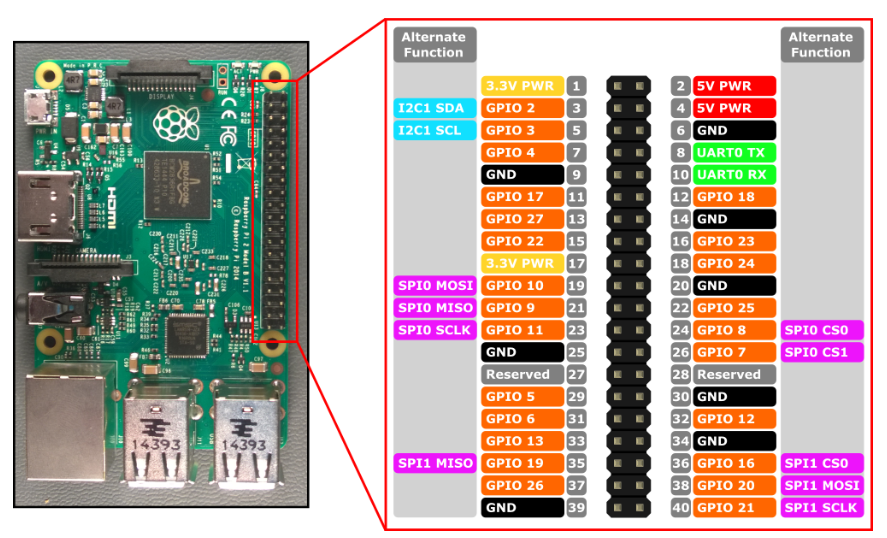
\includegraphics[width=0.7\textwidth]{images/esquemaRaspberry.png}
\caption{Diagrama de pines Raspberry-PI 3.}% 
\label{fig:pinesRaspberry}
\end{figure}


\section{Sistema operativo Raspbian}

Raspbian es un sistema operativo de código abierto basado en Debian, diseñado específicamente para funcionar en la placa R-Pi. Fue creado por el equipo de la Raspberry-Pi Foundation y se ha convertido en el sistema operativo más popular y ampliamente utilizado para la placa R-Pi.

Raspbian es un sistema operativo completo que incluye todas las herramientas y aplicaciones necesarias para realizar tareas típicas de una computadora, como navegar por la web, editar documentos, enviar correos electrónicos, programar y mucho más. La versión más reciente de Raspbian es Raspbian Buster, que se lanzó en 2019.

Entre las características de Raspbian se incluyen:

\begin{enumerate}
\item \textbf{Entorno de escritorio}: Raspbian viene con el entorno de escritorio LXDE, que es un entorno de escritorio ligero y eficiente que funciona muy bien en la placa R-Pi. También es posible instalar otros entornos de escritorio como XFCE, KDE y GNOME.
\item \textbf{Acceso a la terminal}: Además del entorno de escritorio, Raspbian también proporciona acceso a la terminal, lo que permite a los usuarios realizar tareas avanzadas de administración del sistema.
\item \textbf{Soporte para múltiples lenguajes de programación}: Raspbian incluye una gran cantidad de lenguajes de programación, incluyendo Python, Scratch, Ruby, C++, Java, entre otros. Esto hace que la placa R-Pi sea una excelente plataforma para la programación y el desarrollo de software.
\item \textbf{Software preinstalado}: Raspbian incluye una gran cantidad de software preinstalado, como el navegador web Chromium, la suite de ofimática LibreOffice, el reproductor de medios VLC, el cliente de correo electrónico Claws Mail, entre otros.
\item \textbf{Actualizaciones frecuentes}: La Raspberry-Pi Foundation actualiza regularmente Raspbian con parches de seguridad y mejoras de rendimiento.
\item \textbf{Fácil de instalar}: Raspbian se puede descargar gratuitamente desde el sitio web de la Raspberry-Pi Foundation y se puede instalar en la placa R-Pi utilizando una tarjeta SD.
\end{enumerate}


\section{Sensores}

Para este proyecto se utilizarán varios sensores conectados a la placa R-Pi, cada uno de ellos tiene ciertas características propias y utilidades las cuales serán descritas a continuación:

\subsection{MPU6000}

El MPU-6000 es un sensor de movimiento de seis ejes que combina un giroscopio de tres ejes y un acelerómetro de tres ejes en un solo chip. Este sensor es producido por la compañía InvenSense y ha sido utilizado en una gran variedad de aplicaciones, incluyendo drones, robots, consolas de juegos y otros sistemas de navegación.

El giroscopio de tres ejes mide la velocidad angular en cada uno de los tres ejes, permitiendo determinar la orientación y movimiento del objeto en el espacio. Por su parte, el acelerómetro de tres ejes mide la aceleración en cada uno de los tres ejes, lo que permite determinar la posición y velocidad de un objeto.

En cuanto a su conexión con la placa R-Pi, el MPU-6000 se puede conectar a través de un bus de comunicación utilizando protocolo SPI o I2C, lo que lo hace compatible con la mayoría de las placas R-Pi. 

El MPU6000 consta de 7 pines que se dividen en dos grupos: pines de alimentación y de comunicación. 

\begin{enumerate}
\item \textbf{Pines de alimentación}: El MPU-6000 requiere una alimentación de 3.3V, que se suministra a través de:

\begin{itemize}
\item \textit{VCC}: Suministro principal de alimentación y se conecta a una fuente de alimentación de 3.3V.
\item \textit{GND}: Conexión a la tierra de la fuente de alimentación.
\end{itemize}

\item \textbf{Pines de comunicación}: El MPU-6000 se comunica con otros dispositivos a través de los siguientes pines

\begin{itemize}
\item \textit{SCL}: Es el reloj del bus I2C y se utiliza para sincronizar la comunicación de datos.
\item \textit{SDA}: Es el canal de datos del bus I2C y se utiliza para transmitir y recibir datos.
\item \textit{AD0/SDO}: Se utiliza como dirección I2C para seleccionar el MPU-6000 si se están utilizando varios dispositivos I2C en la misma línea de bus. También puede utilizarse como salida de datos para la conexión SPI.
\item \textit{INT}: Se utiliza para enviar interrupciones al microcontrolador de la placa R-Pi para informar sobre cambios en los datos del sensor.
\end{itemize}
\end{enumerate}

En la Figura~\ref{fig:mpu6050} puede observarse el sensor MPU6050 junto con sus pines. 

\begin{figure}[h!]
\centering
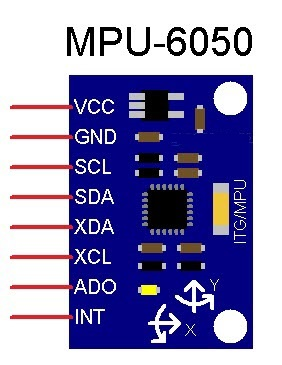
\includegraphics[width=0.3\textwidth]{images/mpu6050.jpg}
\caption[Sensor MPU6050]{Sensor MPU6050 junto con sus respectivos pines.}%
\label{fig:mpu6050}
\end{figure}



\subsection{HMC5983}
el HMC5983 es un sensor de campo magnético de tres ejes producido por la compañía Honeywell. Este sensor es utilizado para medir la intensidad y dirección del campo magnético en tres dimensiones. El HMC5983 cuenta con una resolución de 12 bits para cada eje, lo que le permite proporcionar mediciones precisas y confiables del campo magnético en entornos diversos. Además, cuenta con una alta estabilidad y una respuesta rápida, lo que lo hace adecuado para aplicaciones en las que es necesario detectar pequeñas variaciones en el campo magnético.

En cuanto a su conexión con la placa R-Pi, el HMC5983 se puede conectar a través de un bus de comunicación utilizando únicamente el protocolo I2C.

El sensor HMC5983 cuenta con 5 pines que se dividen en dos grupos: pines de alimentación y de comunicación. A continuación, se describen cada uno de ellos:

\begin{enumerate}
\item \textbf{Pines de alimentación}:  El HMC5983 requiere una alimentación de 3.3V, que se suministra a través de:

\begin{itemize}
\item \textit{VDD}: Es el suministro principal de alimentación y se conecta a una fuente de alimentación de 3.3V.
\item \textit{GND}: Se conecta a la tierra de la fuente de alimentación.
\end{itemize}

\item \textbf{Pines de comunicación}: El HMC5983 se comunica con otros dispositivos a través de:

\begin{itemize}
\item \textit{SCLK}: Es el reloj del bus I2C y se utiliza para sincronizar la comunicación de datos.
\item \textit{SDA}: Es el canal de datos del bus I2C y se utiliza para transmitir y recibir datos.
\item \textit{DRDY}: Se utiliza para enviar interrupciones al microcontrolador de la placa R-Pi para informar sobre cambios en los datos del sensor.
\end{itemize}
\end{enumerate}

En la Figura~\ref{fig:hmc5983} puede observarse el sensor HMC5983 junto con sus pines. 
\vspace{2mm}
\begin{figure}[h!]
\centering
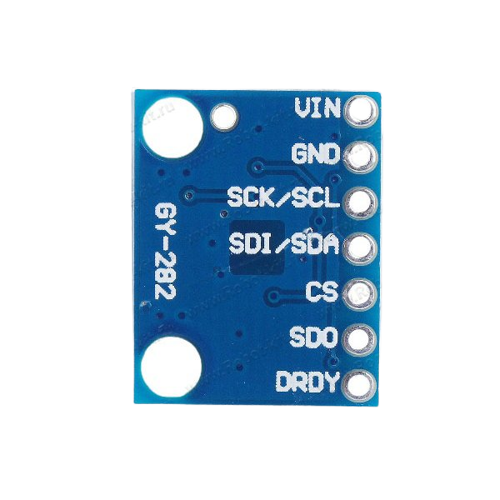
\includegraphics[width=0.4\textwidth]{images/hmc5983.png}
\caption [Sensor HMC5983]{Fotografía del Sensor HMC5983 en la que observan sus pines}
\label{fig:hmc5983}
\end{figure}

\subsection{HC-SR04}
El sensor de distancia HC-SR04 es un componente electrónico utilizado para medir la distancia entre el sensor y un objeto cercano. Se basa en el principio de la emisión y recepción de ondas ultrasónicas.

El HC-SR04 consta de dos partes principales: un transmisor y un receptor ultrasónico. El transmisor emite pulsos de alta frecuencia que no son audibles para los seres humanos. Estos pulsos se propagan en el aire en forma de ondas y cuando encuentran un objeto en su trayectoria, se reflejan hacia el sensor. El receptor del HC-SR04 recibe las ondas reflejadas y las convierte en señales eléctricas. El sensor utiliza un sistema de temporización para medir el tiempo que tarda en recibir la señal reflejada. A partir de esta medición de tiempo, se puede calcular la distancia entre el sensor y el objeto utilizando la fórmula de velocidad del sonido en el aire.

El HC-SR04 cuenta con 4 pines de conexión:
\begin{itemize}
\item \textit{VDD}: Suministra la alimentación al sensor, en este caso debe ser de 5V para su correcto funcionamiento.

\item \textit{Trig}: Se utiliza para iniciar la emisión de los pulsos electromagnéticos utilizados para medir la distancia.

\item \textit{Echo}: Encargado de recibir las señales ultrasónicas reflejadas en el objeto, aquellas que rebotan. Cuando el sensor recibe una señal reflejada, este pin se ocupa de producir un pulso cuya duración es proporcional a la distancia entre el sensor y el objeto.

\item \textit{GND}: Referencia a la tierra de la alimentación, debe estar conectado a un polo negativo para el correcto funcionamiento del sensor.
\end{itemize}

Es importante tener en cuenta que el rango de funcionamiento del HC-SR04 puede variar según las condiciones ambientales y la configuración del sistema. Sin embargo, generalmente puede medir distancias en un rango de varios centímetros hasta varios metros, aunque resulta mas fiable en entornos cerrados sin viento ni ruido y en distancias cortas.
El HC-SR04 es ampliamente utilizado en proyectos de electrónica y robótica, así como en aplicaciones de domótica. Se utiliza para tareas como detección de obstáculos, medición de distancias y sistemas de navegación entre otros. En la Figura~\ref{fig:ultrasonido} puede observarse el sensor HC-SR04 junto con sus pines. 

\vspace{2mm}
\begin{figure}[h!]
\centering
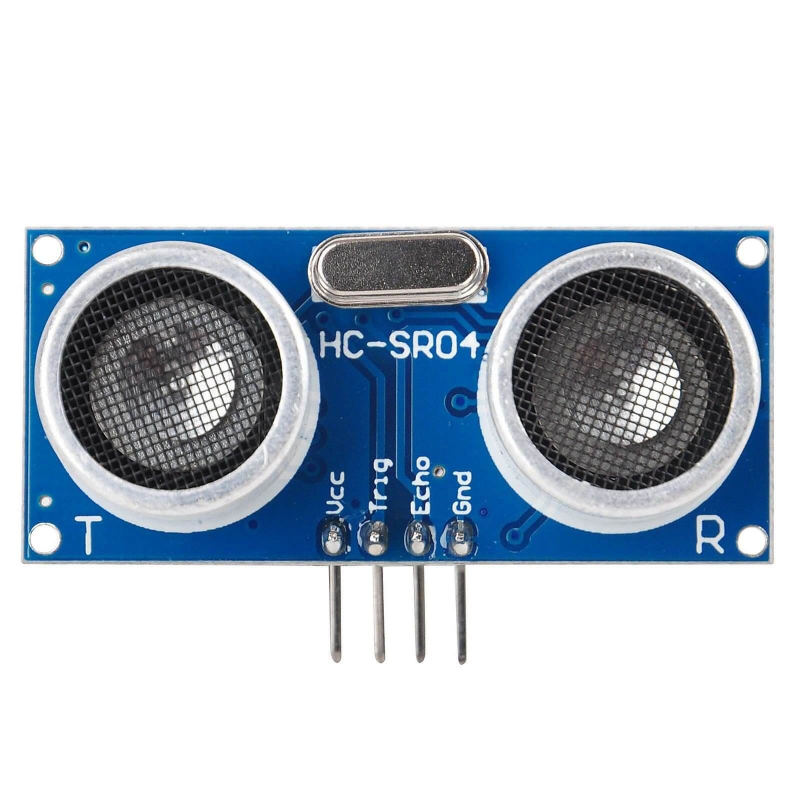
\includegraphics[scale=0.25]{images/HC_SR04}
\caption[Sensor HC-SR04]{Imagen del Sensor HC-SR04 con sus 4 pines observables}%
\label{fig:ultrasonido}
\end{figure}

\section{Apache JMeter}

\label{JMETER} JMeter es una herramienta de prueba de carga y rendimiento de código abierto desarrollada por Apache Software Foundation. Se utiliza principalmente para evaluar y medir el rendimiento de aplicaciones web y servidores, simulando un alto volumen de usuarios y analizando el comportamiento del sistema bajo diferentes cargas.

Algunas características importantes de JMeter son:

\begin{enumerate}
    \item \textbf{Pruebas de carga}: Permite simular un gran número de usuarios simultáneos accediendo a una aplicación web. Esto permite evaluar como responde la aplicación bajo cargas pesadas y determinar su capacidad de manejar un alto volumen de tráfico.
    \item \textbf{Pruebas de rendimiento}: Puede medir el rendimiento de una aplicación web al evaluar los tiempos de respuesta de las solicitudes y analizar métricas como la latencia, el tiempo de procesamiento del servidor y el de descarga de la página entre otros.
    \item \textbf{Escenarios de prueba flexibles}: Ofrece flexibilidad en la creación de escenarios de prueba. Se pueden configurar diferentes hilos de usuarios, establecer la secuencia de solicitudes HTTP y enviar solicitudes POST, GET, PUT y DELETE entre otras.
    \item \textbf{Análisis y generación de informes}: Proporciona informes y gráficos detallados sobre el rendimiento de la aplicación, incluyendo métricas como el tiempo de respuesta promedio, la tasa de errores, el rendimiento por solicitud y la distribución del tiempo de respuesta entre otros. Estos informes ayudan a identificar cuellos de botella y optimizar el rendimiento.
    \item \textbf{Soporte para diferentes protocolos}: Es compatible con varios protocolos, incluyendo HTTP, HTTPS, FTP, JDBC, LDAP, SOAP y JMS entre otros. Esto permite probar diferentes tipos de aplicaciones y servicios.
    \item \textbf{Extensibilidad}: Es altamente extensible y admite la creación de complementos personalizados para ampliar sus capacidades. Además, cuenta con una activa comunidad de usuarios que comparten complementos, scripts y soluciones a problemas comunes.
\end{enumerate}


\chapter{Metodología de trabajo}

\label{sec:metodologia}

En este capítulo se describe la organización del proyecto, las herramientas metodológicas utilizadas y las herramientas usadas para la planificación de actividades, entre ellas destacan: la metodología basada en prototipos, el uso de SysML, los diagramas PERT y Gantt y la descomposición en objetos y tareas. A su vez, se realiza un análisis del proyecto utilizando estas herramientas y el anális de los riesgos.

\section{Metodología basada en prototipos}

La metodología basada en prototipos es un enfoque de desarrollo de proyectos que se utiliza para construir sistemas de software de manera iterativa e incremental. En el contexto de proyectos de software, la metodología basada en prototipos implica la creación de versiones preliminares o prototipos del sistema a lo largo del ciclo de desarrollo. Estos prototipos son versiones simplificadas del sistema final que permiten probar ideas, obtener retroalimentación y validar requisitos antes de la implementación completa.

Uno de los principales beneficios de esta metodología es su enfoque centrado en el usuario. Al desarrollar prototipos, se fomenta la participación activa de los usuarios y se recopila su retroalimentación temprana. Esto permite comprender mejor sus necesidades, expectativas y preferencias, lo que a su vez contribuye a la creación de un sistema final más alineado con sus requerimientos. Además, la metodología basada en prototipos ofrece la ventaja de la rapidez en el desarrollo. Al entregar prototipos funcionales en etapas tempranas del proyecto, se acelera el proceso de validación de conceptos y se reducen los tiempos de respuesta. Esto es especialmente beneficioso en proyectos con plazos ajustados o en entornos donde se requiere una rápida validación de ideas.

La flexibilidad y adaptabilidad son otros aspectos destacados de esta metodología. Los prototipos permiten realizar experimentos y explorar diferentes soluciones antes de comprometerse con una implementación final. Si se detectan problemas o limitaciones, es posible ajustar o cambiar el enfoque sin grandes implicaciones en el sistema completo. Esta flexibilidad facilita la evolución y mejora continua del sistema a medida que se obtiene más conocimiento y experiencia durante el desarrollo.

\subsection{Prototipos contemplados}

Se ha decidido seguir una metodología basada en prototipos debido a sus ventajas en este tipo de proyectos. A continuación se describirán cada uno de los tres prototipos creados que serán divididos en capítulos en el documento:

\begin{enumerate}
   \item \textbf{Prototipo de Exploración}: Se describe el desarrollo inicial del sistema por parte del hardware; la configuración de la Rasperry-Pi así como la conexión de los sensores junto con su implementación y las pruebas realizadas.
    \item \textbf{Prototipo Incremental}: Describe cómo puede utilizarse Erlang sobre la Raspberry-Pi 3 así como diferentes métodos de instalación de este lenguaje sobre la misma, por último, se presentan pruebas realizadas con la placa R-Pi utilizando Erlang.
    \item \textbf{Prototipo Funcional}: Se relata como se ha creado el servidor y cada una de sus partes así como el código que lo implementa, a mayores se describen las pruebas de carga realizadas sobre el mismo para evaluar su rendimiento.

    
\end{enumerate}
\section{Lenguaje de Modelado - SysML}

Para el modelado del análisis y el diseño de los prototipos se utilizará SYSML (\emph{Systems Modeling Language} -- Lenguaje de Modelado de Sistemas, en español). SysML Es un lenguaje de modelado con una componente gráfica importante, ampliamente utilizado en el entorno de la Ingeniería de Sistemas para describir, diseñar y analizar sistemas complejos, se usa especialmente en el diseño de sistemas en ingeniería mecánica, eléctrica, electrónica y de software.

Se basa en el estándar UML (Lenguaje de Modelado Unificado) y utiliza una notación gráfica para describir diferentes aspectos de un sistema, como su estructura, comportamiento, requisitos y análisis. Se compone de nueve tipos de diagramas, cada uno de los cuales se utiliza para describir diferentes aspectos del sistema y son los siguientes:

\begin{enumerate}

\item Diagrama de bloques: Se usa para representar la estructura y las relaciones funcionales entre los componentes de un sistema.
\item Diagrama de bloques internos: Utilizado para para representar la estructura interna de un bloque.
\item Diagrama de flujo de datos: Se utiliza para representar como fluyen los datos a través del sistema.
\item Diagrama de actividades: Se utiliza para modelar el comportamiento del sistema como una secuencia de acciones o actividades.
\item Diagrama de casos de uso: Se utiliza para representar las interacciones entre el sistema y sus usuarios o actores.
\item Diagrama de secuencia: Se utiliza para representar como los diferentes componentes de un sistema interactúan entre sí durante un proceso o escenario específico.
\item Diagrama de estado: Utilizado para representar los diferentes estados que puede tener un objeto en el sistema y como cambia entre ellos.
\item Diagrama de requisitos: Se utiliza para representar los requisitos del sistema y como se relacionan entre sí.
\item Diagrama de asignación de requisitos: Utilizado para representar cómo se asignan los requisitos a los componentes del sistema.
\end{enumerate}
SysML es una herramienta muy útil para el diseño y análisis de sistemas complejos, ya que permite a los ingenieros modelar y comprender el sistema en su totalidad, identificar posibles problemas y evaluar diferentes alternativas de diseño antes de la implementación.

En el diagrama de la Figura~\ref{fig:SYSML} pueden observarse los tipos de diagramas existentes y su respectiva distribución.

\begin{figure}[ht]
\centering
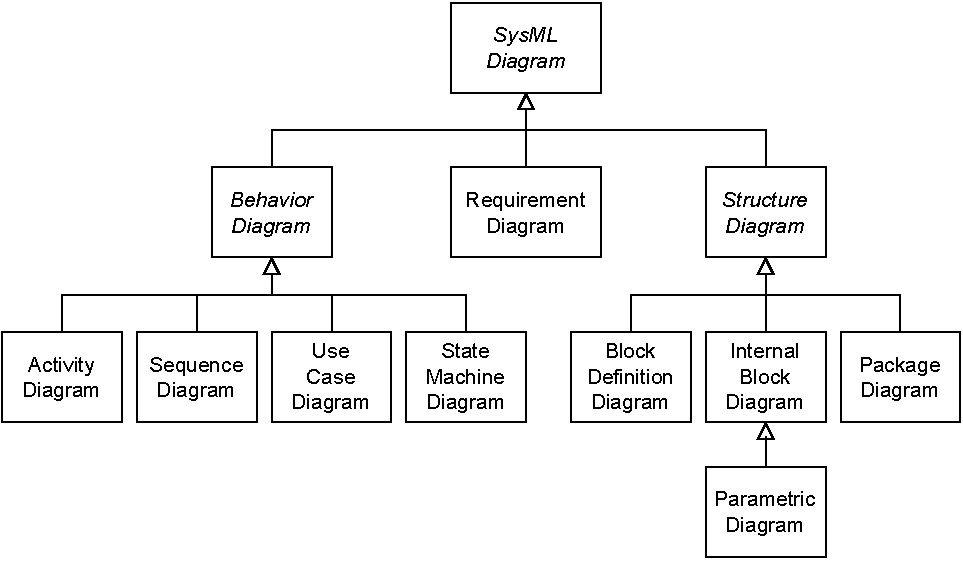
\includegraphics{images/SysMLDiagram.pdf}
\caption[Tipos de diagramas SysML]{Digrama que contiene los tipos de diagramas existentes en SysML.}%
\label{fig:SYSML}
\end{figure}

\section{Planificación del proyecto}

En la siguiente sección se discutirá la planificación del proyecto que se realiza en el Trabajo de Fin de Grado valorando los riesgos y utilizando diagramas de diferentes tipos para representar lo expuesto.

\subsection{Riesgos}%
\label{sec:riesgos}

Dentro de esta sección se analizarán  todos aquellos riegos por los que el proyecto puede verse afectado. Estos riesgos podrían suponer tanto un retraso en la fecha de entrega del proyecto, de alguna de las fases del proyecto hasta llegar a causar un aumento de los costes o incluso la no finalización del mismo. Estos riesgos serán analizados teniendo en cuenta la probabilidad que sucedan, el posible impacto que tengan en el proyecto y las posibles soluciones que puedan existir.

Los riesgos encontrados en este proyecto se pueden ver enumerados en el la Tabla~\ref{tabla:riesgos}. 

\begin{table}[htbp]
\begin{center}
\begin{tabular}{|l|l|}
\hline
\textbf{Código} & \textbf{Descripción} \\
\hline \hline
R-01 & Ausencia puntual del desarrollador. \\ \hline
R-02 & Fallo del equipo de trabajo. \\ \hline
R-03 & Fallo en componentes hardware utilizados. \\ \hline
R-04 & Cierre del laboratorio o centro de trabajo. \\ \hline
R-05 & Pérdida del trabajo realizado. \\ \hline
R-06 & Falta de conocimientos del desarrollador. \\ \hline
R-07 & Falta o retraso de material para el proyecto. \\ \hline
R-08 & Mala planificación del proyecto. \\ \hline
R-09 & Cambios en los requisitos del proyecto. \\ \hline
R-10 & Problemas de interoperabilidad. \\ \hline
\end{tabular}
\caption[Riesgos del sistema]{Enumeración de los riesgos junto con su código.}
\label{tabla:riesgos}
\end{center}
\end{table}

A continuación, se detallará para cada uno de los riesgos encontrados (identificados por su código), el impacto que pueden tener sobre el proyecto, la posibilidad de que ocurran y como podrían solucionarse o moderarse se mostrará en las tablas referenciadas.

\begin{itemize}
    \item \textbf{R-01}: La ausencia temporal del desarrollador debida a cualquier causa (enfermedad o asuntos personales) hace que el riesgo de aumento de duración del proyecto sea directamente proporcional al tiempo que dure la ausencia del mismo (~\ref{tabla:r-01}).
    \item \textbf{R-02}: El fallo del equipo de trabajo, en este caso el PC personal del desarrollador, puede llevar a demoras en el proyecto e incluso derivar en el riesgo R-05 (Pérdida del trabajo realizado) en caso de no haber almacenado información en la nube (~\ref{tabla:r-02}).
    \item \textbf{R-03}: El fallo de componentes hardware es común cuando se realizan trabajos de electricidad y se realizan pruebas sobre los componentes.(\ref{tabla:r-03}).
    \item \textbf{R-04}: El cierre del centro de trabajo, tras los eventos ocurridos durante el COVID-19, resulta más probable que nunca, este riesgo recoge la posibilidad de que el centro de trabajo o investigación tenga que cerrar sus puertas por un tiempo indefinido debido a causas internas o externas al mismo.(\ref{tabla:r-04}).
    \item \textbf{R-05}: Siempre existe la posibilidad de que algún equipo falle y se pierda la información almacenada hasta el momento. Este riesgo haría que el tiempo de entrega del proyecto se retrasara notablemente debido a que recuperar la información o volver a realizar el trabajo requiere mucho tiempo (~\ref{tabla:r-05}).
    \item \textbf{R-06}: La falta de formación del desarrollador para abordar el proyecto haría que este se viese comprometido. La probabilidad de que esto ocurra suele ser baja, pues para que el desarrollador sea seleccionado para el proyecto tiene que demostrar que conoce las herramientas con las que va a trabajar y que tiene conocimientos más que suficientes para llevarlo a cabo (~\ref{tabla:r-06}).
    \item \textbf{R-07}: La falta de material para el proyecto es habitual si no se realiza una planificación adecuada del trabajo, puede influir en el avance del mismo o llevar a cambios de plan. Siempre es recomendable tener suficiente stock para afrontar cualquier proyecto (~\ref{tabla:r-07}).
    \item \textbf{R-08}: La mala planificación del proyecto puede hacer que este se retrase o incluso que no pueda llevarse a cabo, es importante contar con improvistos y realizar una planificación detallada antes de comenzar el trabajo (~\ref{tabla:r-08}).
    \item \textbf{R-09}: Los cambios en los requisitos del proyecto son un riesgo frecuente debido a la modificación de los objetivos o la aparición de imprevistos.(~\ref{tabla:r-09}).
    \item \textbf{R-10}: Los problemas de interoperabilidad son un riesgo común en la realización de este tipo de proyectos debido al uso de diferentes lenguajes, sistemas operativos y componentes, este riego puede crear impedimentos en el flujo del plan de trabajo.(~\ref{tabla:r-10}).
\end{itemize}
    
\begin{table}[htbp]
\begin{center}
\begin{tabular}{|l|p{12cm}|}
\hline
\textbf{R-01} & Ausencia puntual de desarrollador. \\ \hline
\textbf{Impacto} & Bajo. \\ \hline
\textbf{Probabilidad} & Baja. \\ \hline
\textbf{Moderación} & Dar al desarrollador el tiempo que necesite hasta su vuelta. \\ \hline
\textbf{Medidas} & Asignar un desarrollador de respaldo o establecer un plan de contingencia para cubrir las ausencias. También se puede realizar una adecuada documentación y transferencia de conocimientos para que otros miembros del equipo puedan asumir el rol temporalmente.\\ \hline
\end{tabular}
\caption[Riesgo R-01]{Impacto, probabilidad, moderación y medidas del Riesgo R-01}
\label{tabla:r-01}
\end{center}
\end{table}
 
\begin{table}[htbp]
\begin{center}
\begin{tabular}{|l|p{12cm}|}
\hline
\textbf{R-02} & Fallo del equipo de trabajo. \\ \hline
\textbf{Impacto} & Bajo. \\ \hline
\textbf{Probabilidad} & Baja. \\ \hline
\textbf{Moderación} & Tener siempre repuesto de todos los equipos con los que se trabajen y almacenar la información en la nube o realizar copias de seguridad.\\ \hline
\textbf{Solución} & Realizar un mantenimiento preventivo regular de los equipos, incluyendo actualizaciones de software y hardware. Establecer políticas de respaldo y recuperación de datos. Contar con un plan de contingencia que incluya disponibilidad de equipos de respaldo en caso de fallo. Además, es importante contar con un soporte técnico confiable para resolver los problemas de manera rápida y eficiente.\\ \hline
\end{tabular}
\caption[Riesgo R-02]{Impacto, probabilidad, moderación y medidas del Riesgo R-02}
\label{tabla:r-02}
\end{center}
\end{table}  

\begin{table}[htbp]
\begin{center}
\begin{tabular}{|l|p{12cm}|}
\hline
\textbf{R-03} & Fallo en componentes hardware utilizados. \\ \hline
\textbf{Impacto} & Variable (depende de la criticidad del componente). \\ \hline
\textbf{Probabilidad} & Media. \\ \hline
\textbf{Moderación} & Comprobar los componentes antes de utilizarlos y revisar frecuentemente conexiones e implementaciones para evitar cortos o picos de potencia. \\ \hline
\textbf{Solución} & Realizar una adecuada evaluación y selección de los componentes hardware. Mantener un control de calidad en la adquisición y uso de los componentes. En caso de fallo, se debe buscar una solución de reemplazo o reparación lo más rápido posible, considerando la disponibilidad y compatibilidad de los componentes.\\ \hline
\end{tabular}
\caption[Riesgo R-03]{Impacto, probabilidad, moderación y medidas del Riesgo R-03}
\label{tabla:r-03}
\end{center}
\end{table} 

\begin{table}[htbp]
\begin{center}
\begin{tabular}{|l|p{12cm}|}
\hline
\textbf{R-04} & Cierre del laboratorio o centro de trabajo. \\ \hline
\textbf{Impacto} & Alto. \\ \hline
\textbf{Probabilidad} & Baja. \\ \hline
\textbf{Moderación} & No existe forma de moderación hasta que se resuelvan los asuntos que mantienen el centro cerrado. \\ \hline
\textbf{Solución} & Contar con un plan de contingencia que permita trasladar el trabajo a otro lugar en caso de cierre temporal o permanente del laboratorio o centro de trabajo. Esto podría incluir la utilización de instalaciones alternativas, el trabajo remoto o la reubicación de los recursos y equipos necesarios.\\ \hline
\end{tabular}
\caption[Riesgo R-04]{Impacto, probabilidad, moderación y medidas del Riesgo R-04}
\label{tabla:r-04}
\end{center}
\end{table} 

\begin{table}[htbp]
\begin{center}
\begin{tabular}{|l|p{12cm}|}
\hline
\textbf{R-05} & Pérdida del trabajo realizado. \\ \hline
\textbf{Impacto} & Alto. \\ \hline
\textbf{Probabilidad} & Baja. \\ \hline
\textbf{Moderación} & Realizar copias de seguridad periódicas del trabajo realizado, preferiblemente en múltiples ubicaciones o medios de almacenamiento. Utilizar sistemas de control de versiones y almacenamiento en la nube para evitar la pérdida de datos. Implementar prácticas de gestión de cambios adecuadas y realizar pruebas de recuperación de datos de manera regular. \\ \hline
\textbf{Solución} & Recuperar la información en caso de poder o rehacer todo desde la última versión recuperable.\\ \hline
\end{tabular}
\caption[Riesgo R-05]{Impacto, probabilidad, moderación y medidas del Riesgo R-05}
\label{tabla:r-05}
\end{center}
\end{table} 
 
\begin{table}[htbp]
\begin{center}
\begin{tabular}{|l|p{12cm}|}
\hline
\textbf{R-06} & Falta de conocimientos del desarrollador. \\ \hline
\textbf{Impacto} & Alto. \\ \hline
\textbf{Probabilidad} & Baja. \\ \hline
\textbf{Moderación} & Tener siempre bien formado a todo el equipo de desarrollo. \\ \hline
\textbf{Solución} & Proporcionar formación y capacitación adecuada al desarrollador para cubrir las lagunas de conocimiento identificadas. Asignar mentores o expertos en el área para brindar orientación y apoyo. En casos extremos, considerar la contratación de un desarrollador con las habilidades requeridas.\\ \hline
\end{tabular}
\caption[Riesgo R-06]{Impacto, probabilidad, moderación y medidas del Riesgo R-06}
\label{tabla:r-06}
\end{center}
\end{table}

\begin{table}[htbp]
\begin{center}
\begin{tabular}{|l|p{12cm}|}
\hline
\textbf{R-07} & Falta o retraso de material para el proyecto. \\ \hline
\textbf{Impacto} & Bajo. \\ \hline
\textbf{Probabilidad} & Media. \\ \hline
\textbf{Moderación} & Tener siempre suficiente stock de material. \\ \hline
\textbf{Solución} & Realizar una planificación adecuada del proyecto que incluya la identificación y adquisición temprana de los materiales necesarios. Establecer relaciones con proveedores confiables y asegurar acuerdos claros en términos de entrega y disponibilidad de los materiales. En caso de retraso, se puede buscar alternativas o reprogramar las actividades afectadas.\\ \hline
\end{tabular}
\caption[Riesgo R-07]{Impacto, probabilidad, moderación y medidas del Riesgo R-07}
\label{tabla:r-07}
\end{center}
\end{table}

\begin{table}[htbp]
\begin{center}
\begin{tabular}{|l|p{12cm}|}
\hline
\textbf{R-08} & Mala planificación del proyecto. \\ \hline
\textbf{Impacto} & Alto \\ \hline
\textbf{Probabilidad} & Baja \\ \hline
\textbf{Moderación} & Disponer de un plan realista y detallado y contar con improvistos. \\ \hline
\textbf{Solución} & Realizar una planificación detallada y realista del proyecto, considerando todos los aspectos relevantes, como recursos, plazos, objetivos y riesgos. Realizar un seguimiento continuo del progreso y ajustar la planificación según sea necesario. Contar con un equipo de gestión de proyectos competente y utilizar herramientas y metodologías adecuadas para la planificación y el control del proyecto.\\ \hline
\end{tabular}
\caption[Riesgo R-08]{Impacto, probabilidad, moderación y medidas del Riesgo R-08}
\label{tabla:r-08}
\end{center}
\end{table}

\begin{table}[htbp]
\begin{center}
\begin{tabular}{|l|p{12cm}|}
\hline
\textbf{R-09} & Cambios en los requisitos del proyecto. \\ \hline
\textbf{Impacto} & Variable (Depende de la magnitud de los cambios y su impacto en el proyecto). \\ \hline
\textbf{Probabilidad} & Alta. \\ \hline
\textbf{Moderación} & Contar con la posibilidad de modificación de los requisitos.\\ \hline
\textbf{Solución} & Establecer un proceso formal de gestión de cambios que permita evaluar, documentar y aprobar los cambios en los requisitos. Mantener una comunicación constante con los stakeholders para comprender y anticipar posibles cambios. Realizar revisiones regulares de los requisitos y adaptar el plan del proyecto en consecuencia.\\ \hline
\end{tabular}
\caption[Riesgo R-09]{Impacto, probabilidad, moderación y medidas del Riesgo R-09}
\label{tabla:r-09}
\end{center}
\end{table}

\begin{table}[htbp]
\begin{center}
\begin{tabular}{|l|p{12cm}|}
\hline
\textbf{R-10} & Problemas de interoperabilidad. \\ \hline
\textbf{Impacto} & Variable (Depende del grado de dependencia del proyecto de la interoperabilidad). \\ \hline
\textbf{Probabilidad} & Alta \\ \hline
\textbf{Moderación} & Investigar bien los componentes y sistemas antes de utilizarlos.\\ \hline
\textbf{Solución} & Realizar pruebas exhaustivas de interoperabilidad entre los componentes de hardware y software utilizados en el proyecto. Establecer estándares y protocolos de comunicación claros y asegurarse de que todos los elementos del proyecto cumplan con ellos. En caso de identificar problemas de interoperabilidad, trabajar en colaboración con los proveedores y fabricantes para resolverlos o buscar alternativas que sean compatibles.\\ \hline
\end{tabular}
\caption[Riesgo R-10]{Impacto, probabilidad, moderación y medidas del Riesgo R-10}
\label{tabla:r-10}
\end{center}
\end{table}

\clearpage
En la Figura~\ref{fig:matrizRiesgos} se muestra la matriz de probabilidad-impacto de los riesgos que se han identificado mediante su ID, se observa una linea de tolerancia y una distribución por colores para ver de manera visual qué riesgos han de tenerse más en cuenta para tomar medidas antes de que ocurran o disponer de soluciones en caso de que no sea posible evitarlos.

\begin{figure}[h]
\centering
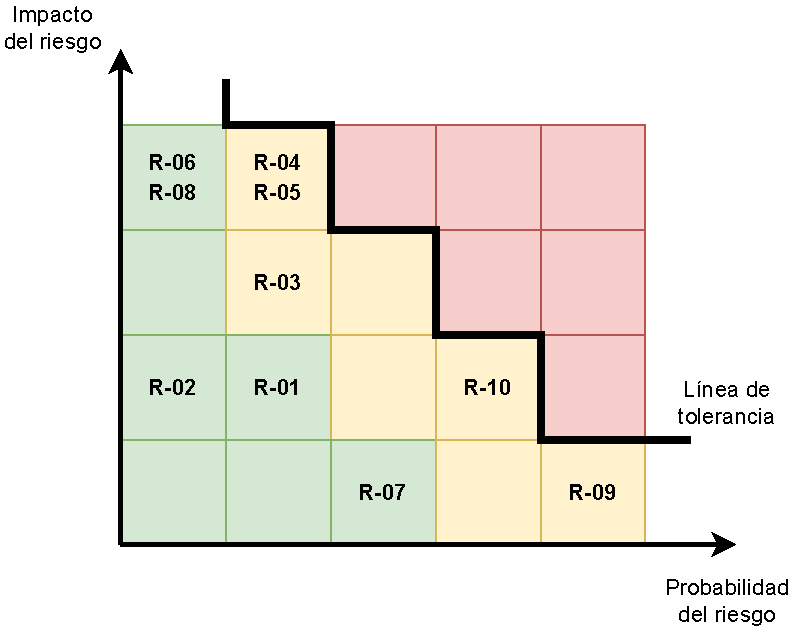
\includegraphics{images/matrizImpacto.pdf}
\caption[Matriz de impacto de riesgos]{Matriz de probabilidad.impacto de riesgos con los IDs de riesgos.}%
\label{fig:matrizRiesgos}
\end{figure}

\newpage

\subsection{Product Breakdown Structure}

La Product Breakdown Structure (PBS) es una herramienta utilizada en la gestión de proyectos para descomponer un producto o proyecto en componentes más pequeños y manejables. Se representa en forma de una estructura jerárquica que muestra la descomposición de alto nivel del producto en sus componentes más detallados.

La PBS se utiliza para definir y organizar las entregas y los elementos del producto. Cada nivel de la estructura representa un nivel de detalle mayor, desglosando el producto en sus partes constituyentes. Los elementos de la PBS se organizan de forma jerárquica, donde los niveles superiores representan las categorías principales y los niveles inferiores representan los elementos más específicos o detallados. Esta herramienta ayuda a visualizar y comprender la estructura del producto, identificar las partes y componentes clave, y establecer una base sólida para la planificación y el control del proyecto. Permite una gestión más efectiva de los recursos, la asignación de responsabilidades y la programación de las actividades necesarias para desarrollar y entregar el producto.

En la Figura~\ref{fig:PBS} pueden observarse el esquema PBS creado para este proyecto, el cual descompone en productos los prototipos necesarios para la realización del mismo así como cada uno de sus componentes.

\begin{figure}[ht]
\centering
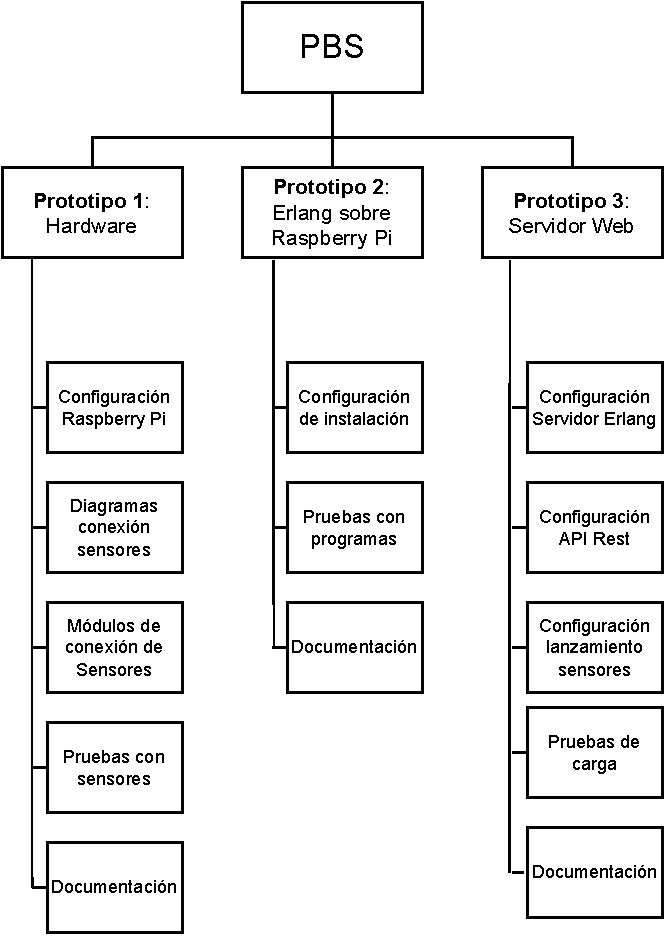
\includegraphics[scale=1.2]{images/PBS.pdf}
\caption[PBS del proyecto]{Esquema de la Product Breakdown Structure (PBS) realizada para la descomposición en objetos del proyecto.}%
\label{fig:PBS}
\end{figure}

\subsection{Work Breakdown Structure}

La Work Breakdown Structure (WBS) es una herramienta clave en la gestión de proyectos que descompone un proyecto en componentes más pequeños y manejables, conocidos como actividades o tareas. La WBS organiza y estructura el alcance del proyecto de manera jerárquica, dividiéndolo en niveles de detalle que representan las diferentes etapas, fases o entregables del proyecto.

La WBS se presenta como un árbol o estructura en la que cada nivel inferior representa una descomposición más detallada de las actividades del proyecto. En la parte superior se encuentra el nivel más general, que representa el alcance principal o los entregables principales del proyecto. A medida que se desciende en la estructura, se especifican las actividades más específicas y se definen las relaciones de dependencia entre ellas. Esta herramienta permite una comprensión clara y organizada del trabajo que debe realizarse en el proyecto. Al descomponer el proyecto en actividades más pequeñas y manejables, se facilita la asignación de responsabilidades a los miembros del equipo y se establece una base para la programación, estimación de recursos y presupuesto.

Los beneficios de utilizar WBS en la gestión de proyectos son diversos. Permite una mejor gestión del alcance, ya que todas las actividades necesarias para completar el proyecto están identificadas y organizadas. Además, ayuda a establecer una secuencia lógica de las actividades y a identificar las dependencias entre ellas. También facilita la comunicación y el seguimiento del progreso del proyecto, ya que proporciona una estructura clara y comprensible para todos los interesados. Permite una asignación eficiente de recursos y tiempo, al permitir la identificación de las actividades críticas y la planificación de los hitos clave del proyecto.

En la Figura~\ref{fig:WBS} pueden observarse el esquema WBS creado para este proyecto, el cual descompone en tareas la creación de los prototipos necesarios para la realización del mismo así como cada una de sus subtareas.

\begin{figure}[ht]
\centering
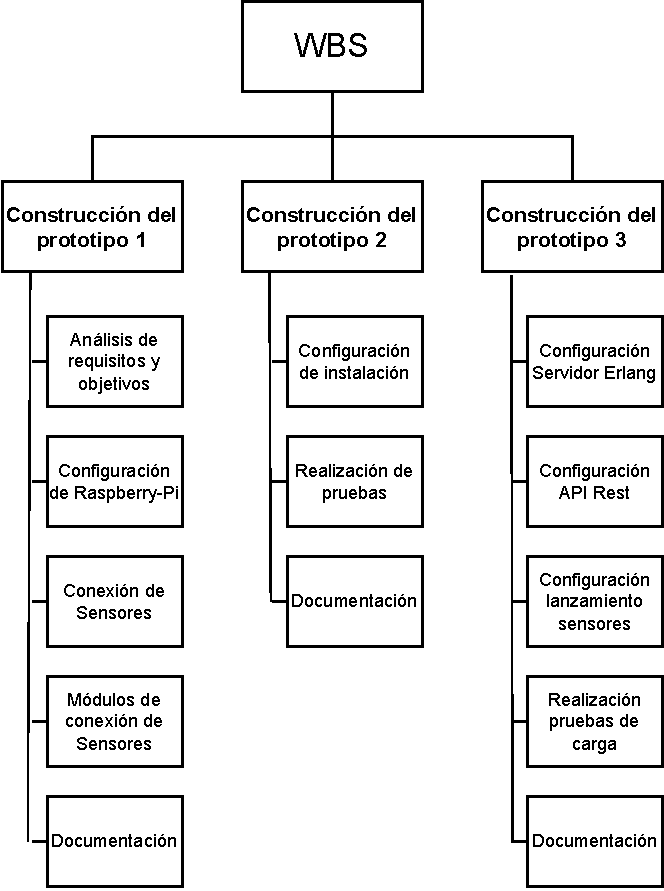
\includegraphics[scale=1.2]{images/WBS.pdf}
\caption[WBS del proyecto]{Esquema de la Work Breakdown Structure (WBS) realizada para la descomposición en tareas del proyecto.}%
\label{fig:WBS}
\end{figure}

\cleardoublepage

\subsection{Red de actividades del proyecto}

En este proyecto se ha plasmado la red de actividades como un diagrama PERT.

Los diagramas PERT (Program Evaluation and Review Technique) son herramientas utilizadas en la gestión de proyectos para visualizar y planificar las actividades y la secuencia de eventos en un proyecto. Estos diagramas se basan en la representación gráfica de las actividades del proyecto, así como en las relaciones de dependencia entre ellas. En un diagrama PERT, las actividades se representan mediante nodos o cajas, y las flechas indican las dependencias y el flujo de trabajo entre las actividades. Cada actividad se representa con su nombre y su duración estimada. Además, se pueden incluir hitos o eventos importantes en el proyecto.

Este tipo de diagramas ayuda a identificar las actividades críticas, es decir, aquellas actividades que tienen un impacto directo en la duración total del proyecto. Estas actividades críticas deben completarse dentro de los plazos establecidos para asegurar que el proyecto se complete a tiempo. Los beneficios de utilizar estos diagramas incluyen una mejor planificación y programación de proyectos, una mayor comprensión de las dependencias entre actividades, la identificación de las actividades críticas, la evaluación de riesgos y la capacidad de ajustar la programación en caso de cambios o retrasos.

En la Figura~\ref{fig:pert} puede observarse el diagrama PERT creado para la representación de las actividades a realizar en el proyecto, en él pueden distinguirse aquellas que tienen dependencias y su flujo de trabajo.

A través de este diagrama puede obtenerse la ruta crítica que se refiere a la secuencia de actividades que determina la duración más larga posible de un proyecto. Es la cadena de tareas que no pueden retrasarse sin retrasar la finalización del proyecto en su conjunto, es por ello que a estas actividades se les debe dar un plazo algo superior para evitar retrasos importantes en la duración del proyecto. La ruta obtenida es la siguiente:\\

\dirtree{%
.1 Configuración inicial Raspberry-Pi.
.2 Elección y conexión de sensores con Raspberry-Pi.
.3 Creación módulos de sensores.
.4 Creación Servidor Erlang.
.5 Configuración API REST.
.6 Lanzamiento sensores desde servidor.
.7 Pruebas finales.
.8 Documentación prototipo final.
}

\begin{figure}[p]
\centering
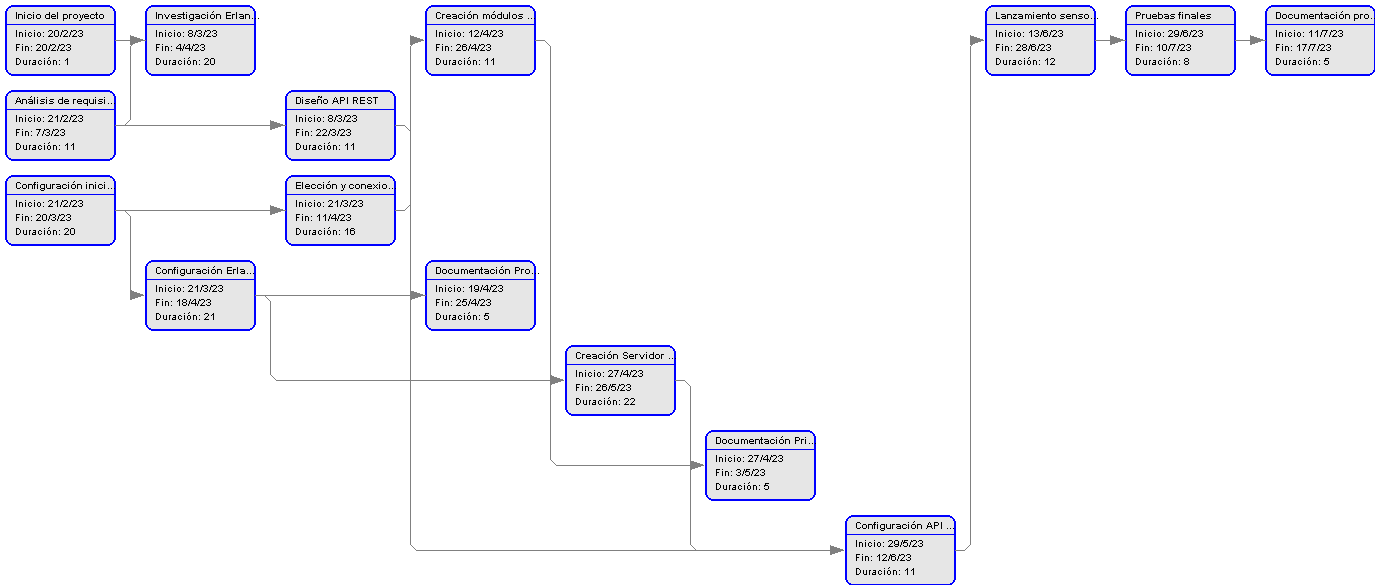
\includegraphics[scale=0.5,angle=90]{images/Pert.png}
\caption[Diagrama PERT]{Diagrama PERT de descomposición de actividades del proyecto}%
\label{fig:pert}
\end{figure}

\clearpage
\subsection{Diagrama de Gantt}

Un diagrama de Gantt es una herramienta de gestión de proyectos que muestra la planificación y programación de las actividades a lo largo del tiempo. Consiste en una representación gráfica en forma de barras horizontales que muestran la duración de cada actividad y su ubicación en el calendario. En un diagrama de Gantt, el eje horizontal representa el tiempo, generalmente en unidades de días, semanas o meses. Cada actividad se representa como una barra en el diagrama, donde la longitud de la barra indica la duración de la actividad. Las barras se colocan en el tiempo correspondiente en el eje horizontal y se pueden superponer si hay actividades que se solapan en el tiempo. Además de mostrar la duración de las actividades, el diagrama de Gantt también puede mostrar otras información relevante, como las dependencias entre actividades, los hitos importantes del proyecto y las fechas límite. Las dependencias se representan mediante flechas que indican la secuencia en la que las actividades deben llevarse a cabo.

Uno de los beneficios de estos diagramas es su capacidad para visualizar claramente el flujo de trabajo y la secuencia de actividades en un proyecto. Permite a los miembros del equipo y a los stakeholders comprender rápidamente el cronograma del proyecto y las fechas clave. También ayuda a identificar posibles cuellos de botella y retrasos, lo que permite realizar ajustes en la planificación si es necesario. Por otro lado, resalta su capacidad para mostrar la asignación de recursos. Además de mostrar la duración de las actividades, se pueden agregar barras adicionales para representar la asignación de personal, equipo u otros recursos a cada actividad. Esto ayuda a tener una visión completa de cómo se utilizan los recursos a lo largo del tiempo y facilita la gestión de la capacidad y la carga de trabajo.

En la Figura~\ref{fig:gantt} puede observarse el diagrama Gantt creado para la representación de las actividades a realizar en el proyecto, en él puede observarse la fecha de inicio del proyecto (20/02/2023) así como las principales actividades y sus dependencias en el marco temporal establecido para el proyecto.


\begin{figure}[p]
\centering
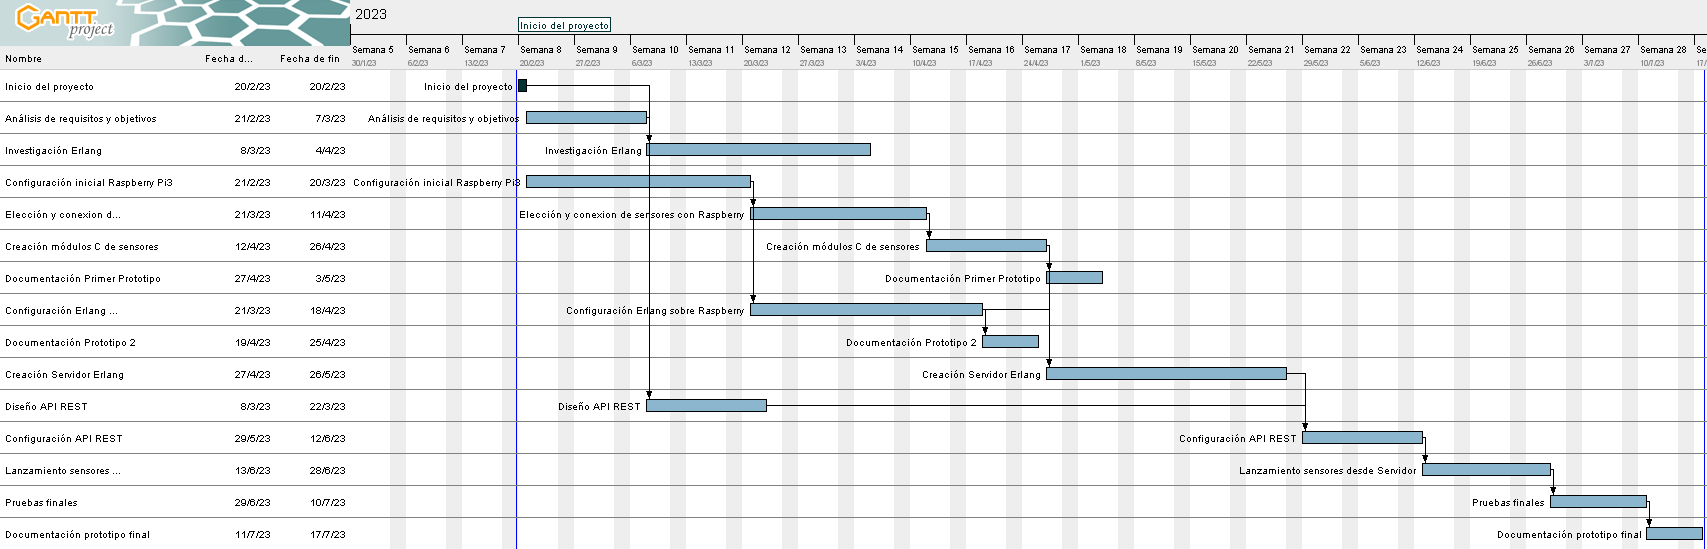
\includegraphics[height=0.32\textheight,angle=90]{images/TFGGantt.png}
\caption[Diagrama de Gantt]{Diagrama Gantt de la planificación del proyecto}%
\label{fig:gantt}
\end{figure}

\clearpage
\section{Recursos a emplear}

Tras la definición de actividades se deben analizar los recursos necesarios para el desarrollo del poryecto, estos se pueden diferenciar en tres tipos: Humanos, materiales y tecnológicos.

\subsection{Recursos humanos}%
\label{sec:recHumanos}

Estos recursos se miden contando las horas de trabajo de los desarrolladores, por ello, utilizando las actividades definidas y el tiempo disponible, se realiza una estimación del esfuerzo en horas de trabajo para desarrollarlas. Se estima la realización del proyecto en un periodo de 4 meses y 300 horas totales para la realización de los tres prototipos. Es por ello que se disponen de 88 días hábiles por lo que se deberán emplear una media de 3.4 horas diarias para la la finalización a tiempo del proyecto. 
El coste de estas horas se ha obtenido a través de la referencia bibliográfica \cite{Cowork2023}.

En la Tabla~\ref{tab:costSoft} puede observarse la estimación de horas necesarias para la realización de las diferentes actividades principales del proyecto.

\begin{table}[h]
\begin{center}
\begin{tabular}{|l|c|}
\hline
\rowcolor{gray!20}
\textbf{Software} & \textbf{Cantidad (Horas)} \\
\hline
Configuración de Raspberry-Pi & 30 \\
\hline
Conexión de sensores & 30\\
\hline
Programación de sensores & 55\\
\hline
Pruebas de frecuencia & 40 \\
\hline
Programación Servidor Erlang & 70\\
\hline
Pruebas de uso y cumplimiento requisitos & 30 \\
\hline
Documentación & 45 \\
\hline
\rowcolor{gray!20}
\textbf{Total} & \textbf{300}\\
\hline
\end{tabular}
\caption[Estimación de horas de trabajo]{Estimación de la distribución de horas de trabajo por actividades.}%
\label{tab:costSoft}
\end{center}
\end{table}

\subsection{Recursos materiales}%
\label{sec:recHardware}

En cuanto a los recursos materiales para el desarrollo del proyecto se requiere de:

\begin{itemize}
    \item Laboratorio (coworking).
    \item Ordenador (renting).
    \item Monitor (renting).
    \item Hardware (Adquirido).
    \item Licencias Software (Adquirido).
\end{itemize}

El hardware estimado que debe adquirirse es el mostrado en la Tabla~\ref{tab:recHard}.
\begin{table}[h]
\begin{center}
\sffamily
\begin{tabular}{|l|c|r|}
\hline
\rowcolor{gray!20}
\textbf{Componente} & \textbf{Cantidad}  & \textbf{Precio}  \\
\hline
Kit Raspberry-Pi 3 & 1 & 80\officialeuro  \\
\hline
Sensores & 5 & 35\officialeuro \\
\hline
Jumper Wire Cables & 3x40 pcs & 8\officialeuro \\
\hline
Resistencias 2.2K\(\Omega\) & 10 pcs & 2\officialeuro \\
\hline
Resistencias 1K\(\Omega\) & 10 pcs & 2\officialeuro \\
\hline
\rowcolor{gray!20}
\textbf{Total} & & \textbf{127\officialeuro} \\
\hline
\end{tabular}
\caption[Costes de componentes hardware]{Costes estimados de Hardware necesarios para la realización del proyecto}%
\label{tab:recHard}
\end{center}
\end{table}

\subsection{Recursos tecnológicos}

Para el desarrollo del proyecto se requiere del siguiente software de pago, en esta sección no aparece todo aquel software gratuito utilizado:

\begin{itemize}
    \item Licencia de Windows 10 Profesional.
    \item Licencia Office.
\end{itemize}

\subsection{Costes estimados del proyecto}

Por último, se presentan los costes del proyecto sumando todos los tipos de recursos requeridos, el sueldo por hora para los recursos humanos (trabajo) se ha obtenido mediante la Web Talent \cite{Cowork2023}. Para ello se ha escogido la media de los sueldos de los puestos especializados en cada fase, el resultado obtenido ha sido 19\officialeuro/hora.

En la Tabla~\ref{tab:costesTot} puede observarse el conjunto de todos los recursos junto con la cantidad necesaria de tiempo y su coste. Se ha obtenido una estimación total del proyecto de 7122\officialeuro.


\begin{table}[h]
\begin{center}
\sffamily
\begin{tabular}{|l|c|c|r|}
\hline
\rowcolor{gray!20}
\textbf{Recurso} & \textbf{Cantidad} & \textbf{Unidad} & \textbf{\officialeuro Total}  \\
\hline
Recurso Humano &  300 horas & 19\officialeuro/hora  \cite{Cowork2023}& 6000 \\
\hline
Laboratorio Coworking &  4 meses & 125\officialeuro/mes & 365  \\
\hline
Ordenador Renting &  4 meses & 125\officialeuro/mes & 200  \\
\hline
Monitor renting &  4 meses & 25\officialeuro/mes & 100  \\
\hline
Licencia Windows 10&  1 &  260\officialeuro & 260  \\
\hline
Licencia Office &  1 &  70\officialeuro & 70  \\
\hline
Recursos Hardware &  Tabla~\ref{tab:recHard} & 127\officialeuro & 127  \\
\hline
\rowcolor{gray!20}
\textbf{Total} & & & \textbf{7122\officialeuro} \\
\hline
\end{tabular}
\caption{Costes totales estimados del proyecto}%
\label{tab:costesTot}
\end{center}
\end{table}









\chapter{Requisitos y Análisis del problema}

\section{Requisitos funcionales}
Un requisito funcional es una declaración que describe una función o característica específica que debe cumplir un sistema o software, estos requisitos definen qué debe hacer el sistema y cómo debe comportarse en términos de funcionalidad. En la Tabla~\ref{tab:requisitosfunionales} se podrán ver los requisitos funcionales del sistema.
\begin{table}[htbp]

\begin{tabular}{p{2cm} p{12cm}}
RF-01 & El sistema deberá implementar un dispositivo hardware, compuesto por un dispositivo Raspberry-Pi con sensores conectados, para la toma de medidas. \\ \\
RF-02 & El sistema deberá contar con un servidor Erlang donde los usuarios puedan interactuar.\\ \\
RF-03 &  El sistema deberá tomar medidas de distancia mediante un sensor de ultrasonidos.\\ \\
RF-04 &  El sistema deberá tomar medidas de cabeceo con respecto al campo magnético mediante un sensor magnetómetro.\\ \\
RF-05 &  El sistema deberá tomar como mínimo 10 medidas por segundo para hacer la demostración en tiempo real.\\ \\
RF-06 &  El sistema deberá almacenar los datos obtenidos en archivos de texto para su posterior análisis.\\ \\
RF-07 &  El servidor deberá poder comunicarse con la placa R-Pi para lanzar la lectura de los sensores.\\ \\
RF-08 & El sistema deberá poder comunicarse con el servidor para poder los archivos con la información de las medidas.\\ \\
RF-09 & El servidor deberá permitir al usuario consultar la descripción de los sensores. \\ \\
RF-10 & El servidor deberá permitir al usuario interactuar mediante una arquitectura API REST. \\ \\
RF-11 & El servidor deberá permitir al usuario visualizar los archivos de datos obtenidos por los sensores. \\ \\
RF-12 & El servidor deberá permitir al usuario modificar los parámetros de lanzamiento de los sensores. \\ \\
RF-12 & El servidor deberá ofrecer un manual de uso de la interfaz al usuario. \\ \\



\end{tabular}
\label{tab:requisitosfunionales}
\caption{Requisitos Funcionales}
\end{table}

\section{Requisitos no funcionales}

Se entiende como requisito no funcional, dentro del ámbito de la ingeniería del software, a un requisito que describe una cualidad o restricción que debe cumplir el sistema en términos de rendimiento, seguridad, usabilidad, mantenibilidad u otras características no directamente relacionadas con la funcionalidad específica. Por lo tanto, se trata de las restricciones o condiciones impuestas por el usuario que ordena desarrollar este sistema.
En la Tabla~\ref{tab:requisitosnofunionales} se enumeran los requisitos no funcionales del sistema.
\begin{table}[htbp]

\begin{tabular}{p{2cm} p{12cm}}
RNF-01 & El sistema deberá utilizar un dispositivo de medición de datos diseñado sobre Raspberry-Pi.\\ \\
RNF-02 & El sistema deberá utilizar un servidor creado con lenguaje Erlang OTP.\\ \\
RNF-03 & El servidor deberá ser eficiente en el procesamiento de solicitudes y proporcionar una respuesta rápida a los usuarios.\\ \\
RNF-04 &  El sistema debe ser compatible con diferentes plataformas y navegadores web, asegurando una amplia accesibilidad para los usuarios.\\ \\
RNF-05 & El sistema deberá ser fácilmente usable e intuitivo una vez leído el manual de funcionamiento.\\ \\
RNF-06 &  El sistema deberá ser confiable, asegurando la respuesta esperada.\\ \\
RNF-07 & El sistema deberá almacenar la información recogida durante el tiempo de muestreo. \\ \\
RNF-08 &  El sistema debe estar disponible y operativo la mayor parte del tiempo, minimizando los períodos de inactividad.\\ \\
RNF-09 & El sistema debe garantizar la seguridad de los datos transmitidos y almacenados..\\ \\
RNF-10 & El código del sistema debe ser modular, legible y fácilmente mantenible para facilitar futuras actualizaciones y correcciones.\\ \\
RNF-11 & El sistema estar diseñado para ser fácilmente escalable, de esta manera pueden añadirse más sensores con posterioridad.\\ \\



\end{tabular}
\label{tab:requisitosnofunionales}
\caption{Requisitos No Funcionales}
\end{table}

\newpage

\section{Diagramas SysML del modelo}

\subsection{Diagrama de paquetes del modelo}

En el diagrama presentado en la Figura~\ref{fig:diagramaPaquetes}, se muestra el Diagrama de Paquetes del modelo del sistema que incluye aquellos modelos que se han elaborado para mostrar el sistema y los requisitos del mismo, este diagrama podría ser ampliable e incluir más elementos pero se ha decidido mostrar únicamente aquellos que realmente muestran información importante para la realización del proyecto. Este diagrama incluye:

Diagramas de casos de uso y secuencia para mostrar el comportamiento y dos diagramas de descripción de bloques que muestran la descripción de la estructura del sistema a alto nivel. En el caso de las pruebas no se han realizado diagramas pero se incluye su descripción textual en lo sucesivo.


\begin{figure}[h!]
\centering
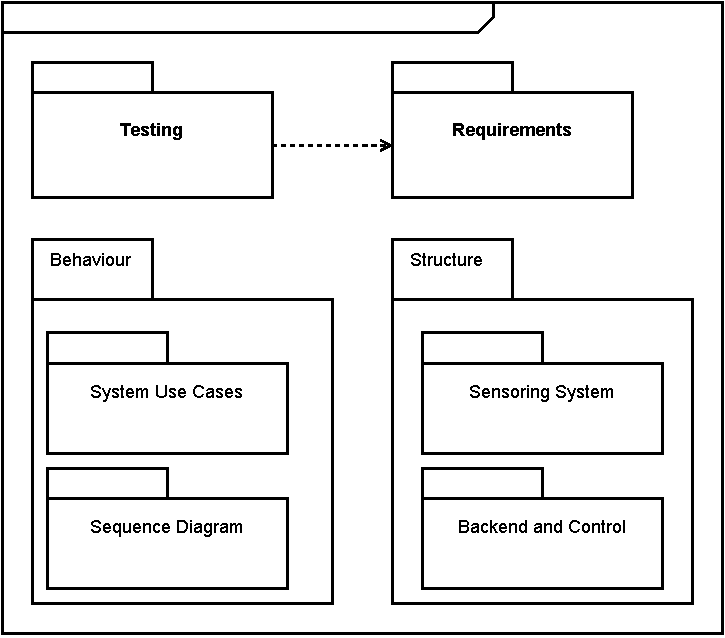
\includegraphics{images/diagramaDePaquetes.pdf}
\caption{Diagrama de paquetes}%
\label{fig:diagramaPaquetes}
\end{figure}

\subsection{Diagrama de casos de uso}

Un diagrama de casos de uso es una herramienta utilizada en el análisis y diseño de sistemas para representar las interacciones entre los actores (usuarios o sistemas externos) y un sistema en particular. Proporciona una visión general de las funciones que el sistema ofrece y cómo se relaciona con los usuarios.

En un diagrama de casos de uso, los casos de uso se representan como elipses y los actores como figuras externas al sistema. Las flechas indican las interacciones entre los actores y los casos de uso, mostrando qué funciones realiza el sistema en respuesta a las acciones de los usuarios. El objetivo principal de un diagrama de casos de uso es capturar los requisitos funcionales del sistema y comprender cómo los usuarios interactúan con él. Ayuda a identificar las diversas formas en que los usuarios pueden utilizar el sistema y los escenarios en los que se involucran.

En el caso de nuestro proyecto contamos con dos actores: el administrador y el usuario.
\begin{itemize}
    \item \textbf{Administrador}: Encargado de configurar el servidor, disponiendo de la posibilidad de añadir o eliminar sensores al sistema, a su vez puede realizar las mismas actividades que realiza un usuario.
    \item \textbf{Usuario}: Puede acceder a la interfaz web para: lanzar la lectura de los sensores, ver el manual de uso, ver las especificaciones de los sensores o ver los datos obtenidos por los mismos.
\end{itemize}

Puede observarse el diagrama de casos de uso en la Figura~\ref{fig:usecases}


\begin{figure}[h!]
\centering
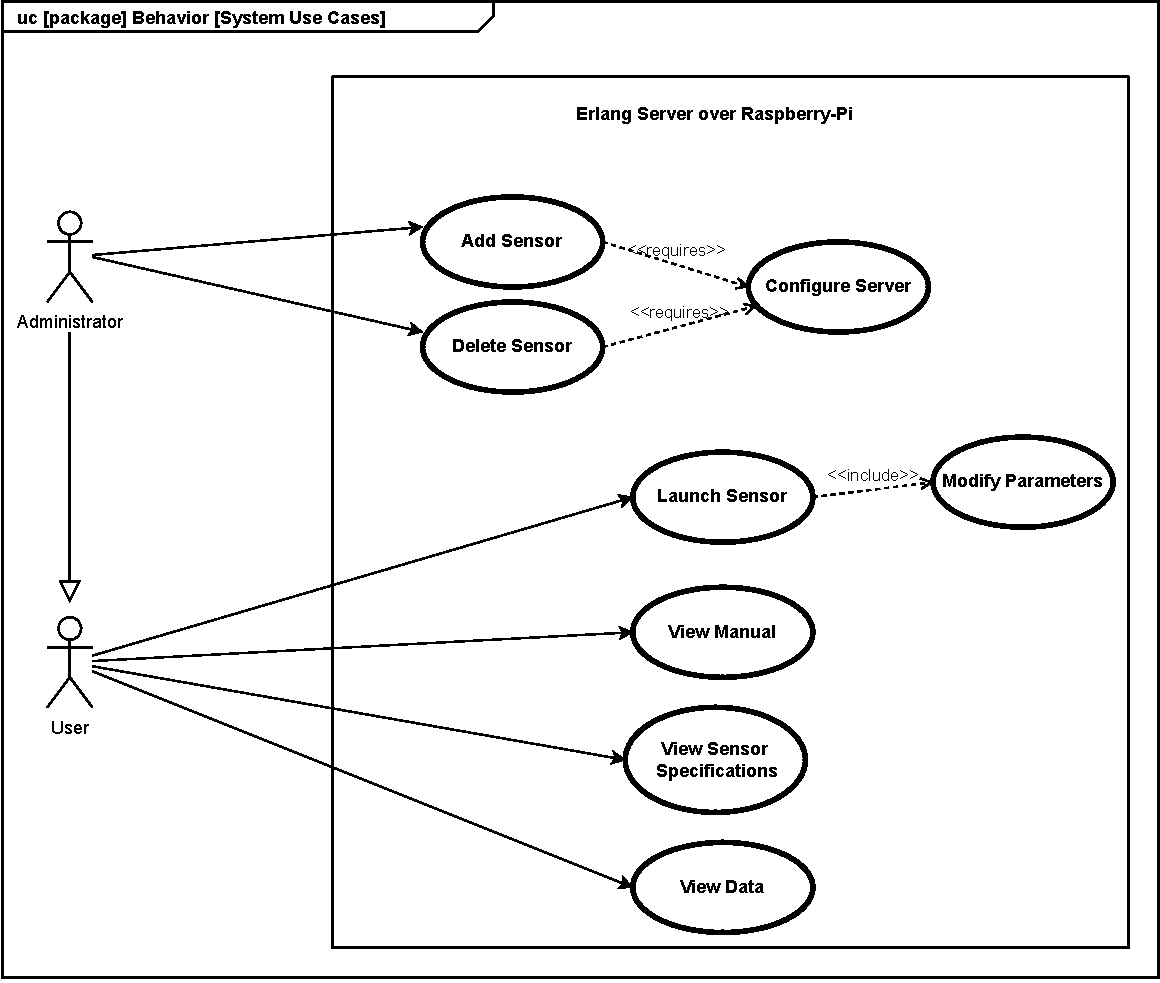
\includegraphics[width=\textwidth]{images/casosUso.pdf}
\caption{Diagrama de Casos de Uso del sistema}%
\label{fig:usecases}
\end{figure}

\clearpage

\subsection{Diagrama de secuencia}

En el segundo diagrama de comportamiento del sistema, el diagrama de secuencia observado en la Figura~\ref{fig:diagramaSecuencia}, se pueden identificar varios pasos clave:

\begin{figure}[t]
\centering
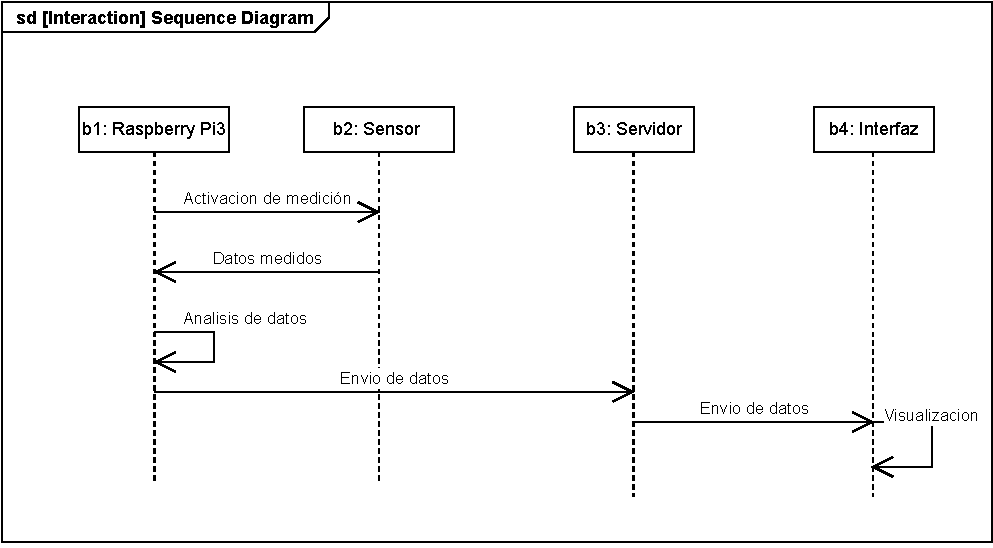
\includegraphics[width=\textwidth]{images/diagramaSecuencia.pdf}
\caption{Diagrama de Secuencia}%
\label{fig:diagramaSecuencia}
\end{figure}



\begin{enumerate}
\item Activar medición: Se activa el sensor para que comience a medir los datos.

\item Datos medidos: El sensor envía los datos medidos a la placa R-Pi a través de un protocolo de comunicación adecuado (como puede ser I2C).

\item Analizar datos en C: La placa R-Pi recibe los datos del sensor, los procesa a través de un código en C que los analiza y transforma en un formato adecuado para su almacenamiento y posterior envío al servidor.

\item Datos analizados: Una vez que el código en C ha analizado los datos, los envía de vuelta a la placa R-Pi en un formato adecuado para su almacenamiento.

\item Guardar en archivo: Cuando la placa R-Pi ha recibido los datos analizados, los guarda en un archivo local en la placa de desarrollo para su posterior envío al servidor.

\item Enviar archivo: la placa R-Pi envía el archivo con los datos analizados al servidor a través de una conexión adecuada (como puede ser una conexión por Internet).

\item Recibir archivo: el servidor recibe el archivo con los datos analizados enviado por la placa R-Pi.

\item Analizar archivo: el servidor analiza los datos recibidos en el archivo y genera los resultados.

\item Resultados: el servidor envía los resultados a la interfaz para que sean visualizados por el usuario.
\end{enumerate}


\subsection{Diagrama de bloques: Sensoring System}

El diagrama de bloques del sistema se encuentra disponible en la Figura~\ref{fig:diagramaBloques}, en él pueden observarse los objetos principales del sistema y como estos se comunican entre sí. El sensor es el dispositivo encargado de recolectar los datos, estos datos se transmiten al Web Service a través de un protocolo I2C de conexión el cual puede almacenar hasta 7 dispositivos, de ahí su cardinalidad.


\begin{figure}[h!]
\centering
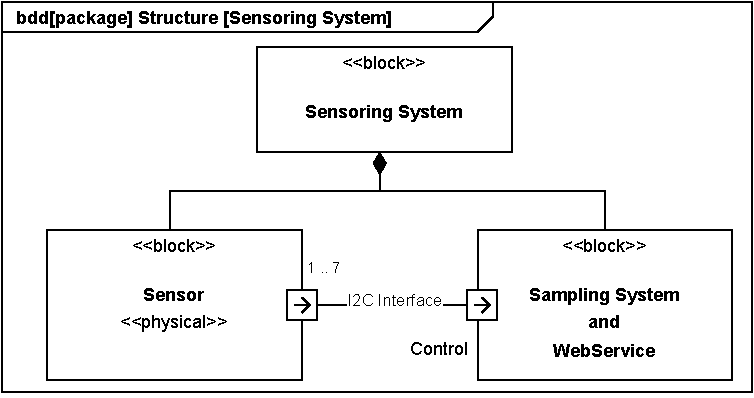
\includegraphics[scale=1.2]{images/bloques.pdf}
\caption{Diagrama de bloques: Sensoring System.}%
\label{fig:diagramaBloques}

\end{figure}


\subsection{Diagrama de bloques: Control y Backend}


En la Figura~\ref{fig:diagramaControl} se puede observar el otro diagrama de bloques que describe el Backend y Control del sistema, en él puede observarse la comunicación entre los diferentes componentes y los protocolos utilizados, a su vez puede verse cuál de ellos tiene el control sobre la comunicación.

\begin{figure}[h!]
\centering
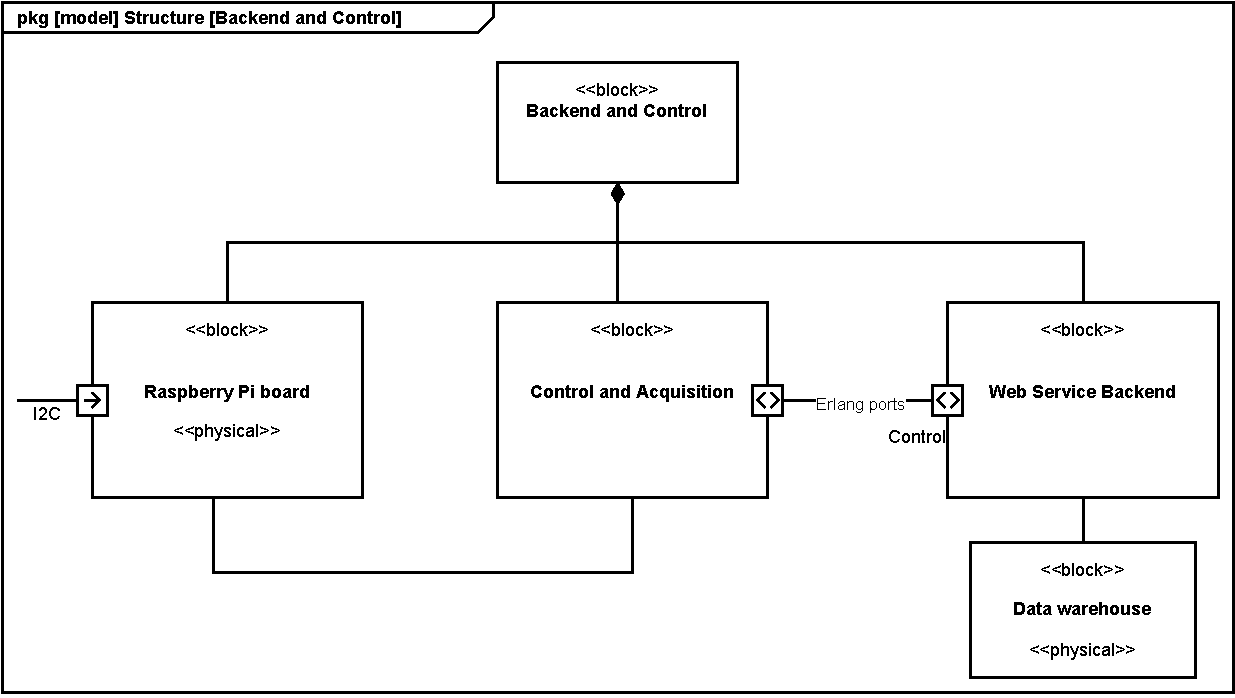
\includegraphics[width=\textwidth]{images/model.pdf}
\caption{Diagrama de Bloques: Control y Backend.}%
\label{fig:diagramaControl}

\end{figure}




\chapter{Prototipo de Exploración}\label{cap.prototipoExploracion}

En este capítulo se describe la creación del primer prototipo del proyecto, el prototipo de exploración, en él se explica la configuración de la placa R-Pi, la conexión de los sensores y el código utilizado para la lectura de los mismos. Por último se realizan algunas pruebas para demostrar el correcto funcionamiento y su rendimiento.


\section{Desarrollo del Sistema}

\subsection{Configuración de la Raspberry-Pi}
En primer lugar, debe instalarse en la placa de desarrollo el sistema operativo que vamos a utilizar, existen varias opciones posibles pero se ha optado por la más habitual denominada Raspbian o Raspberry-Pi OS.
La tarea resulta bastante sencilla simplemente siguiendo los pasos de la página oficial, a través de la cual disponemos de la opción automática de usar un instalador (RaspberryPi Imager) en el que seleccionaremos el lugar de almacenamiento del sistema (la tarjeta Micro SD) y el sistema operativo elegido y únicamente tendremos que esperar a que haga todo el trabajo de escritura. La Figura~\ref{fig:raImager} muestra la interfaz del programa Raspberry Pi Imager.

\begin{figure}[tbh]
\centering
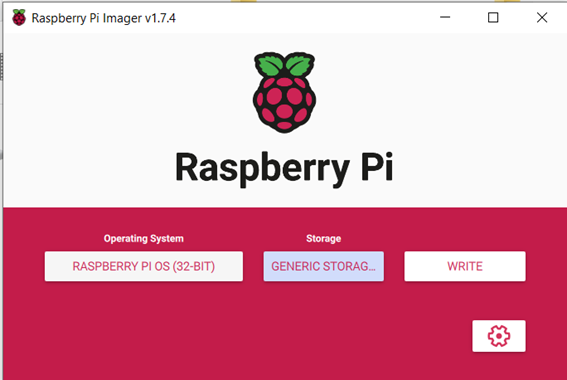
\includegraphics[scale=0.6]{images/raspberryImager}
\caption[Interfaz instalación Raspberry Pi]{Interfaz principal de la aplicación de instalación de sistemas operativos Raspberry Pi: {\protect\tt imager}.}%
\label{fig:raImager}
\end{figure}

Una vez terminado el proceso de instalación, podemos proceder a introducir la tarjeta Micro-SD en la placa R-Pi y realizar todas las conexiones pertinentes para poder arrancar el sistema. Para ello se debe conectar la alimentación, red por cable o posteriormente configurar la WIFI, un teclado, un ratón y un monitor a través de HDMI. 
El proceso es sencillo, seleccionar idioma, zona horaria...etc. Tras unos minutos dispondremos de la placa R-Pi con el sistema operativo plenamente funcional y con una interfaz gráfica muy similar a un Linux.

Tras realizar estos pasos podemos proceder a modificar la contraseña de la placa R-Pi para securizarla a través del menú de configuración o a través de terminal ejecutando el comando\\
\begin{lstlisting}[style=terminal]
sudo raspi-config\end{lstlisting}

Otro punto importante a modificar es en el apartado <<Interface Options>>, es en esta sección a través de la cual debemos activar o desactivar las diferentes opciones de interfaces.\\

En las Figuras \ref{fig:cambioContra} y \ref{fig:interfaceOpt} pueden observarse las opciones de modificación de contraseña y configuración de interfaces comentadas anteriormente.

\begin{figure}[tbh]
\centering
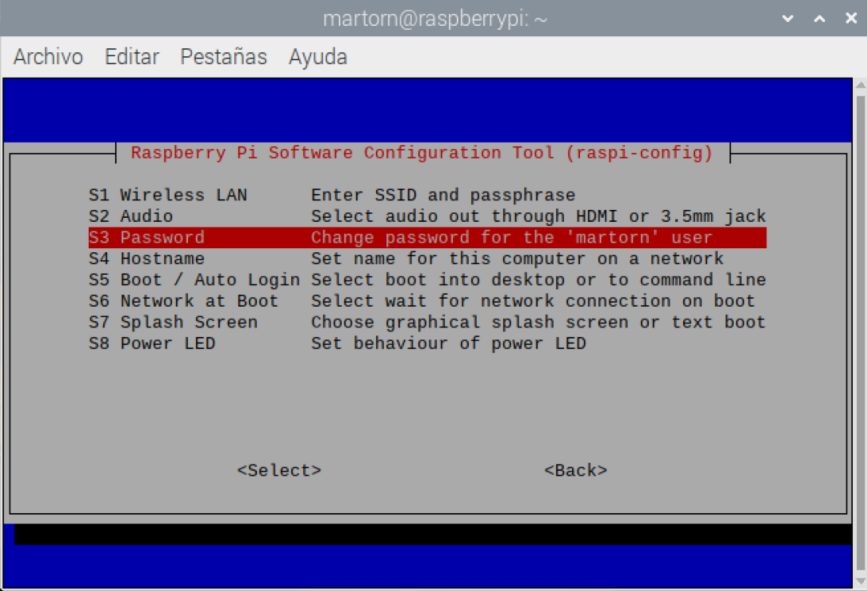
\includegraphics[scale=0.7]{images/raspiConfigPass}
\caption[Cambio de contraseña de Raspberry Pi]{Menú de configuración inicial para realizar el cambio de contraseña: {\protect\tt Password}.}%
\label{fig:cambioContra}
\end{figure}

\begin{figure}[tbh]
\centering
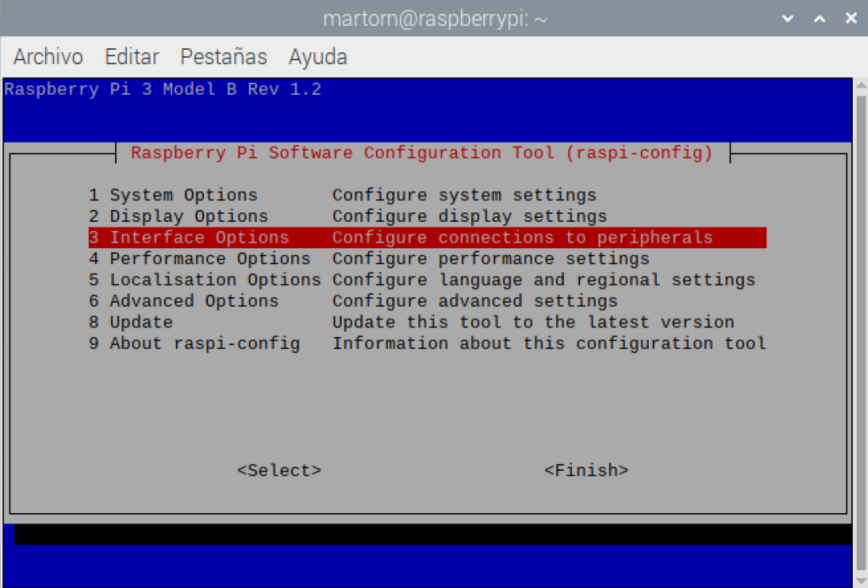
\includegraphics[scale=0.7]{images/raspiConfigInterface}
\caption[Configuración de interfaz de Raspberry-Pi]{Menú de configuración inicial para configuración de interfaces: {\protect\tt Interface Options}.}%
\label{fig:interfaceOpt}
\end{figure}

En la configuración de interfaces activaremos: \textbf{SSH, VNC, SPI, I2C, Serial y Remote GPIO.}

En primer lugar, SSH y VNC permitirán contactar de manera remota con la placa R-Pi para poder acceder a ella o programar, por otro lado, SPI e I2C serán los protocolos de conexión con los sensores que utilizaremos, por ello es importante que estén activos, las otras dos opciones darán acceso a otras funcionalidades de la placa.

\section{Conexión con Raspberry-Pi}
\subsection{VNC Viewer}

Una de las opciones más sencillas para trabajar cómodamente con la placa R-Pi, evitar tantas conexiones y el uso de un monitor externo, es el uso de la herramienta VNC Viewer, con ella se podrá visualizar directamente el entorno gráfico de la placa R-Pi exactamente igual que si estuviéramos conectados por HDMI, en el caso de usar SSH no dispondríamos de entorno visual, es por ello que esta herramienta resultará muy útil.

Para poder utilizar VNC Viewer se debe descargar de la página oficial el instalador y seguir los pasos de instalación, una vez instalada únicamente se debe configurar la conexión con la placa R-Pi determinando la dirección IP de la misma con su respectivo usuario y contraseña como se observa en la Figura~\ref{fig:VNC} para así poder acceder. Tras realizar estos pasos dispondremos de la interfaz gráfica plenamente operativa desde nuestro PC.

En resumen, con esta herramienta obtenemos el beneficio de disponer de la interfaz gráfica totalmente funcional desde nuestro PC como si de una máquina virtual se tratara y a su vez nos evitamos la conexión del teclado, el ratón y el monitor por HDMI a la placa R-Pi.

\begin{figure}[tbh]
\centering
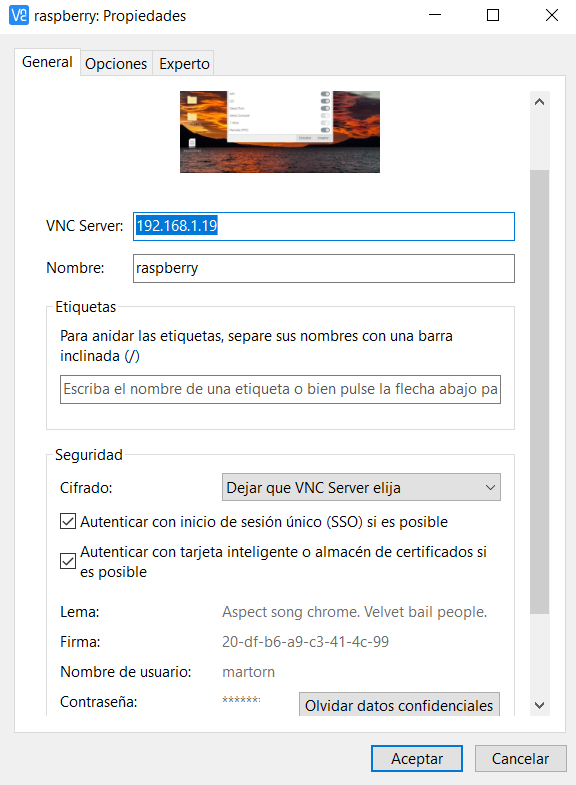
\includegraphics[scale=0.8]{images/vnc.png}
\caption[Configuración de VNC Viewer]{Pestaña propiedades de la aplicación VNC Viewer: Configuración de ejemplo para la conexión con la placa R-Pi.}%
\label{fig:VNC}
\end{figure}

\subsection{Conexión USB to Serial Port}
Otra de las opciones para realizar la comunicación con la placa de desarrollo es la utilización de un adaptador USB a Serial, en concreto un dispositivo FTDI232, mostrado en la Figura~\ref{fig:serial}.

\begin{figure}[tbh]
\centering
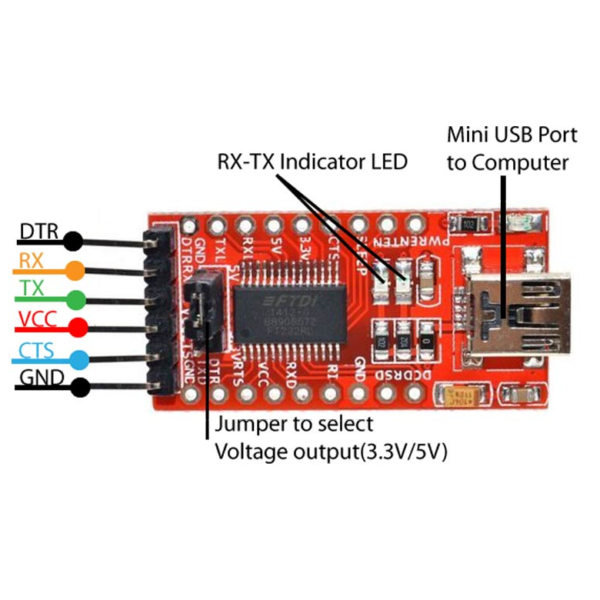
\includegraphics[scale=0.5]{images/serial.png}
\caption[Descripción pines para FTDI232]{Imagen con descripción de los pines del dispositivo para conexión Serial-FTDI232.}%
\label{fig:serial}
\end{figure}

Este dispositivo permite el envío de información directamente al puerto USB del dispositivo al que lo conectemos, en este caso un PC. Para que funcione debe realizarse la conexión de tres de sus pines; Rx, Rt y GND, la alimentación la recoge del puerto USB. Estos pines deben conectarse a la placa R-Pi al contrario; Rx a Rt y viceversa. Rx y Rt son los pines 14 y 15 de la placa R-Pi como puede observarse en la Figura~\ref{fig:Rxrt} figura. 

\begin{figure}[tbh]
\centering
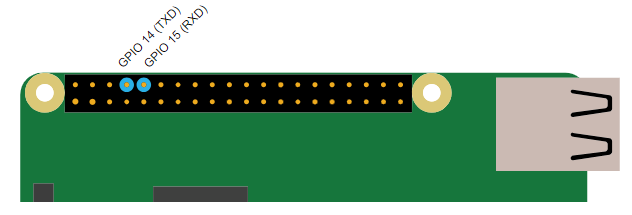
\includegraphics[scale=0.7]{images/serialRasp.png}
\caption[Configuración RX y RT en Raspberry Pi 3]{Localización de los pines RX y RT en el modelo de Raspberry-Pi 3.}%
\label{fig:Rxrt}
\end{figure}

En la placa R-Pi debe activarse la opción de conexión serial que vimos en el apartado de configuración de la Raspberry-Pi, en este caso ya se encuentra activada.

Una vez realizada la conexión, debemos revisar el administrador de dispositivos de nuestro PC para encontrar dónde se ha conectado el dispositivo, en nuestro caso se trata de COM7 (Figura ~\ref{fig:com7}), una vez conocida la linea serie ya podemos configurar el programa Putty para que lea en esa dirección (Figura~\ref{fig:puttyConf}) y por tanto podamos acceder a la placa R-Pi.

\begin{figure}[tbh]
\centering
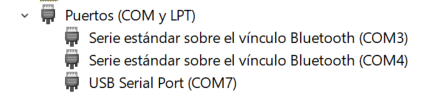
\includegraphics[scale=1]{images/serialCOM.png}
\caption[Puertos COM y LPT en Windows]{Captura de lista de puertos COM y LPT en el administrador de dispositivos de Windows, puede observarse USB Serial Port como COM7.}%
\label{fig:com7}
\end{figure}

\begin{figure}[tbh]
\centering
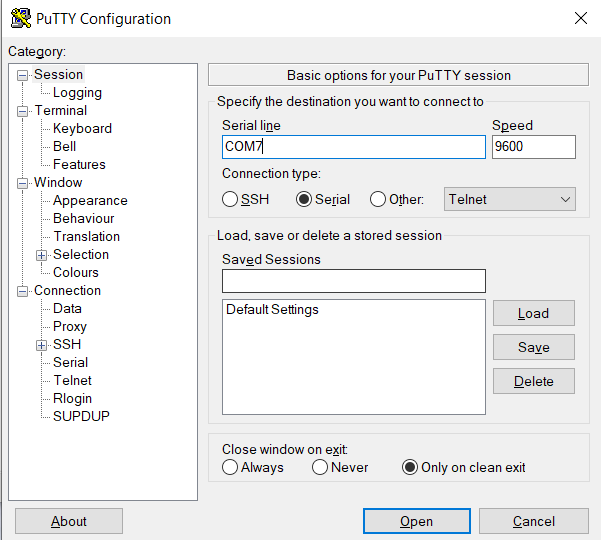
\includegraphics[scale=0.8]{images/putty.png}
\caption[Configuración de Putty para conexión con Raspberry-Pi]{Configuración de la herramienta Putty en Windows para realizar la conexión con la placa R-Pi a través del puerto serie ({\protect\em Serial Port}).}%
\label{fig:puttyConf}
\end{figure}

Al lanzar Putty obtenemos la salida deseada, la placa R-Pi solicita el inicio de sesión mediante usuario y contraseña y, en este momento ya podemos hacer pleno uso de la misma como si estuviéramos en su terminal, en la Figura~\ref{fig:puttyOK} se muestra su visualización:

\begin{figure}[tbh]
\centering
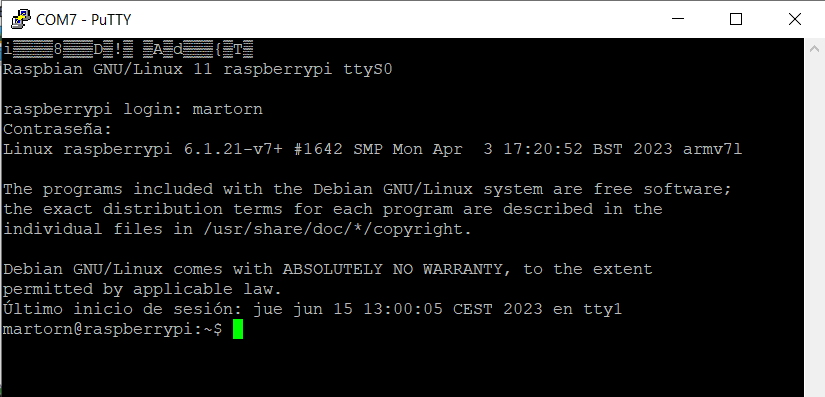
\includegraphics[scale=0.9]{images/puttyOK.png}
\caption[Primer acceso de Putty a Raspberry-Pi]{Visualización del primer acceso desde el terminal de Putty a la placa R-Pi a través de Serial Port.}%
\label{fig:puttyOK}
\end{figure}


\section{Conexión y configuración de los sensores}

Para afrontar el problema se plantean las posibles opciones disponibles, el primer paso es realizar una búsqueda de información sobre el sensor que se desea utilizar, sobre como conectarlo a la placa R-Pi y sobre el lenguaje a utilizar.

En cuanto a las opciones sobre protocolos existen dos: I2C y SPI, para este tipo de proyectos se usa de manera más habitual I2C ya que no se mueve gran densidad de datos y requiere de menos conexiones que SPI, igualmente se barajan ambas posibilidades, es por ello que veremos sus ventajas y desventajas y valoraremos cuál es la mejor opción para este tipo de proyecto. A continuación, se presentan algunos puntos a considerar:

\textbf{Número de dispositivos:} Si es necesario conectar múltiples dispositivos a un bus de comunicación, I2C generalmente es más adecuado. I2C utiliza solo dos líneas de comunicación (SCL y SDA), lo que permite conectar varios dispositivos en el mismo bus utilizando direcciones únicas. Al contrario, SPI requiere una línea separada para cada dispositivo conectado, lo que puede limitar la cantidad de dispositivos que se pueden conectar directamente.

\textbf{Velocidad de transferencia:} SPI tiende a tener una velocidad de transferencia más rápida que I2C. En SPI, la velocidad de transferencia se puede ajustar para adaptarse a los requisitos específicos, mientras que I2C tiene una velocidad máxima establecida.

\textbf{Complejidad y pines requeridos:} I2C generalmente requiere menos pines que SPI. Como se mencionó anteriormente, I2C utiliza sólo dos líneas de comunicación, mientras que SPI requiere al menos cuatro líneas (MISO, MOSI, SCK y SS). Si se trabaja con recursos limitados en términos de pines de conexión o es un requisito utilizar la mínima complejidad de cableado, I2C puede ser una mejor opción.

\textbf{Tolerancia al ruido:} I2C tiende a ser más tolerante al ruido que SPI. El protocolo I2C utiliza una topología de bus abierto con drenaje abierto, lo que proporciona una mayor inmunidad al ruido eléctrico. Por otro lado, SPI utiliza señales más nítidas y puede ser más susceptible a interferencias electromagnéticas. Si se trabaja en un entorno ruidoso o con señales propensas a interferencias, I2C podría ser más adecuado.

Por otro lado, en cuanto a los posibles lenguajes de programación a utilizar se han barajado tres posibilidades: Erlang, C y Python. Se harán pruebas con cada uno de ellos para valorar cuál es la mejor opción ya que el objetivo es que se realice una lectura rápida de los datos y de la manera más eficiente.
En estos casos es importante conocer o descubrir la existencia de módulos o librerías ya existentes que nos ofrezcan soluciones más rápidas y sencillas que podamos utilizar para nuestros prototipos.

\subsection{Configuración sensor HMC5983}

El primer prototipo se creará utilizando un sensor HMC5983 y realizando la conexión a través del protocolo I2C, las características de este sensor estarán descritas en la sección correspondiente al mismo. 
Partiendo de la base inicial, el primer paso será realizar las conexiones del sensor a los pines de la placa R-Pi, para utilizar este protocolo necesitamos conectar cuatro de los pines del sensor; VCC (positivo), GND (negativo), SCL y SDA (transmisión de datos). Estos pines serán conectados a la placa R-Pi como se indica en la Figura~\ref{fig:5983Rasp}.

\begin{figure}[th]
\centering
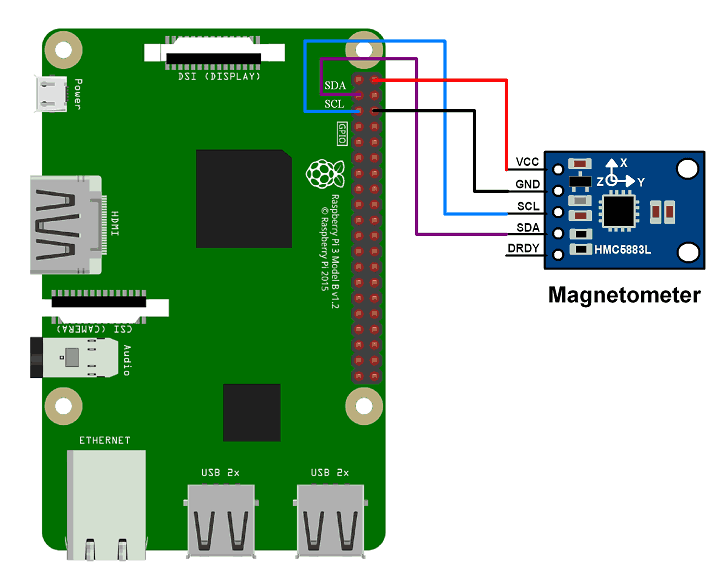
\includegraphics[scale=0.5]{images/conexionRaspHMC5983}
\caption[Conexión HMC5983 a Raspberry-Pi]{Diagrama de conexiones del sensor HMC5983 a Raspberry-Pi 3.}%
\label{fig:5983Rasp}
\end{figure}

Para comprobar que las conexiones se han realizado correctamente, en primer lugar se debe activar el protocolo I2C de la placa R-Pi entrando en su configuración, para ello ejecutamos el comando 
\begin{lstlisting}[style=terminal]
raspi-config
\end{lstlisting}
posteriormente, accedemos a la configuración de interfaces y activamos I2C (enable), tras la realización de estos pasos la placa R-Pi está preparada para recibir datos utilizando este protocolo.Por último, es necesario saber si hemos conectado correctamente el sensor, para ello se ejecuta el comando 

\begin{lstlisting}[style=terminal]
i2cdetect -y 1
\end{lstlisting}
 y se nos mostrará una tabla en la que, en caso de estar todo bien conectado, aparecerá un registro activo como se muestra en la Figura~\ref{fig:i2cDetect}. Podemos observar que se trata de la dirección 0x1E por lo que será aquí donde deberá direccionarse la recogida de datos del sensor
\begin{figure}[th]
\centering
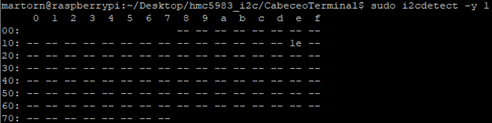
\includegraphics{images/i2cdetect.png}
\caption[Comando <<i2cdetect>> con sensor HMC5983]{Salida del comando <<i2cdetect>> en el terminal de la placa R-Pi tras la conexión con el sensor HMC5983.}%
\label{fig:i2cDetect}
\end{figure}


\subsubsection{Código Python Sensor HMC5983}

El código de este sensor en Python resulta bastante sencillo de encontrar en multitud de páginas web, incluso en la oficial del propio sensor, gracias a esto podemos utilizar códigos ya existentes para adaptarlos a nuestras necesidades lo que ahorra gran cantidad de tiempo. La placa R-Pi no dispone de Python por lo que debe instalarse siguiendo las metodologías habituales, una vez instalado puede pasarse a probar si el código creado lee correctamente nuestro sensor magnetómetro HMC5983. 

El código es sencillo pero consta de varias partes importantes que han de tenerse en cuenta para la posterior programación en otros lenguajes, es por ello que se adjunta el código completo Python que devuelve el cálculo del cabeceo del sensor por terminal para poder así explicar cada una de ellas.

En la primera sección, aparte de importar los módulos necesarios se crean las variables que serán usadas como direcciones de los registros, estas son direcciones representadas como un número hexadecimal obtenidas del datasheet del sensor. El siguiente paso es inicializar el sensor, para ello se establecen ciertos valores en los registros de configuración que establecen el modo y la ganancia del sensor.

La función $read\_raw\_data()$, se utiliza, como su nombre indica, para leer los datos sin procesar, toma la dirección del registro como argumento y lee dos bytes de datos (uno alto y uno bajo), posteriormente, combina los dos bytes en un valor de 16 bits y ajusta el signo en caso de ser necesario.

Tras la realización de estos pasos, se lanza la función que inicializa el sensor para que este empiece a leer de manera continuada, esta función obtiene los datos de los ejes X, Y y Z pero estos aún están sin procesar, es por ello que se calcula el cabeceo utilizando la función \textit{math.atan2()} que devuelve el ángulo en radiantes y por último se suma la declinación al ángulo calculado. Por último, se comprueba si el ángulo es mayor que 2$\pi$ o si es negativo para ajustarlo en caso de ser necesario.\\

\lstset{language=Python, breaklines=true, basicstyle=\footnotesize}
\begin{lstlisting}[frame=single]

import smbus #import SMBus module of I2C
from time import sleep  #import sleep, used for reading frequency
import math

Register_A     = 0              #Address of Configuration register A
Register_B     = 0x01           #Address of configuration register B
Register_mode  = 0x02           #Address of mode register

X_axis_H    = 0x03              #Address of X-axis MSB data register
Z_axis_H    = 0x05              #Address of Z-axis MSB data register
Y_axis_H    = 0x07              #Address of Y-axis MSB data register
declination = -0.00669          #define declination angle of location where measurement going to be done
pi          = 3.14159265359     #define pi value

def Magnetometer_Init():
        #write to Configuration Register A
        bus.write_byte_data(Device_Address, Register_A, 0x70)

        #Write to Configuration Register B for gain
        bus.write_byte_data(Device_Address, Register_B, 0xa0)

        #Write to mode Register for selecting mode
        bus.write_byte_data(Device_Address, Register_mode, 0)
	
def read_raw_data(addr):
    
        #Read raw 16-bit value
        high = bus.read_byte_data(Device_Address, addr)
        low = bus.read_byte_data(Device_Address, addr+1)

        #concatenate higher and lower value
        value = ((high << 8) | low)

        #to get signed value from module
        if(value > 32768):
            value = value - 65536
        return value


bus = smbus.SMBus(1) 	
Device_Address = 0x1e   # HMC5983 Address

Magnetometer_Init()     # initialize HMC5883L magnetometer 

print (" Reading Heading Angle")

while True:
   
        #Read Accelerometer raw value
        x = read_raw_data(X_axis_H)
        z = read_raw_data(Z_axis_H)
        y = read_raw_data(Y_axis_H)

        heading = math.atan2(y, x) + declination
        
        #Due to declination check for >360 degree
        if(heading > 2*pi):
                heading = heading - 2*pi

        #check for sign
        if(heading < 0):
                heading = heading + 2*pi

        #convert into angle
        heading_angle = int(heading * 180/pi)

        print ("Heading Angle = %d" %heading_angle)
        sleep(0.5)

\end{lstlisting}


En la salida obtenida del sensor observada en la Figura~\ref{fig:salidaHMCP}, se puede ver que es correcta y los ángulos se obtienen en bucle hasta finalizar la ejecución del programa de manera manual, a mayores, la frecuencia de lectura es modificable cambiando el valor de sleep() medido en segundos, en este caso 0.5. 

\begin{figure}[th]
\centering
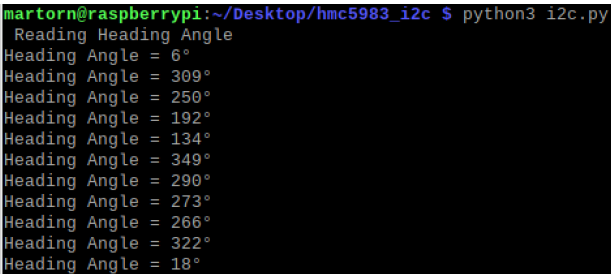
\includegraphics{images/salidaHMC5983Python.png}
\caption[Salida código Python sensor HMC5983]{Visualización de la salida en terminal tras la ejecución del código del sensor HMC5983 implementado en Python.}%
\label{fig:salidaHMCP}
\end{figure}

\subsubsection{Código C Sensor HMC5983}

El código C se ha creado a semejanza del código Python visto anteriormente, a diferencia del anterior, este dispone de la posibilidad de pasarle dos argumentos, el tiempo durante el cual queremos que se lean datos y la frecuencia de lectura de los mismos; a mayores, este programa almacena los datos de cabeceo en un archivo externo que será utilizado para su visualización en el servidor.

Se han encontrado más dificultades para encontrar información sobre este código en este lenguaje, se ha observado que la utilización de Python para la programación de este tipo de sensores es mucho más frecuente. Un punto positivo es que al disponer con anterioridad del programa Python se ha podido utilizar como base. La mayor diferencia y el gran beneficio de la utilización del lenguaje C en el caso de este proyecto es la compatibilidad que tiene con Erlang, esto será una gran ventaja de cara a la programación del servidor ya que debe comunicarse con el programa que ejecuta los sensores desde la placa R-Pi.

El funcionamiento del código es similar, se inicializa el sensor y se calcula el cabeceo con los datos obtenidos de los ejes X, Y y Z, como se comentó anteriormente. En este código se han añadido algunas mejoras con respecto al anterior: en primer lugar, se permite la introducción de dos argumentos: el tiempo y la frecuencia y en segundo lugar, se crea el archivo en el que se escribirán los datos obtenidos del sensor. El siguiente paso es crear una función que compruebe si el tiempo introducido en el argumento es mayor que el tiempo transcurrido, de esta manera puede conseguirse que el programa termine en caso de llegar al límite de tiempo. Por último se introduce el parámetro de la frecuencia en la variable del $time\_sleep$s.\\

A la hora de compilar el código C, antes de ejecutarlo, es importante enlazar las bibliotecas \textit{pigpio} (Controladora de pines GPIO) y \textit{libm} (funciones matemáticas adicionales), para ello se debe ejecutar el comando de compilación gcc añadiendo -lpigpio -lm como sigue:\\
\begin{lstlisting}[style=terminal]
gcc -o nombreEjecutable nombrePrograma.c -lpigpio -lm
\end{lstlisting}

\lstset{language=C, breaklines=true, basicstyle=\footnotesize}
\begin{lstlisting}[frame=single]
//Importacion de librerias necesarias
#include <stdio.h>
#include <stdlib.h>
#include <pigpio.h>
#include <math.h> 

//Definicion de los registros a utilizar.
//la direccion se ha obtenido ejecutando el comando i2cdetect -y 1 sobre la linea de comandos.
#define HMC5983_ADDR 0x1E 
#define HMC5983_REG_X_MSB 0x03
#define HMC5983_REG_Y_MSB 0x07
#define HMC5983_REG_Z_MSB 0x05
#define PI 3.14159265358979323846

int main(int argc, char *argv[])
{
    if(argc !=3){
        printf("Uso:sudo %s [tiempo_lectura] [ratio_lectura]\n", argv[0]);
        return 1;
    }
    
    double tiempo = atof(argv[1]);
    double ratio = atof(argv[2]);
    
    if (gpioInitialise() < 0) {
        printf("Error al inicializar la biblioteca pigpio\n");
        return 1;
    }

    int handle = i2cOpen(1, HMC5983_ADDR, 0);
    if (handle < 0) {
        printf("Error al configurar el dispositivo I2C.\n");
        return 1;
    }
   
    i2cWriteByte(handle, 0x00); //Configuracion del modo continuo
   

//Creacion del archivo en el que se escribiran los datos
    FILE *fp;
    fp = fopen("/home/martorn/Desktop/hello_erlang/src/sensorData/angulosCabeceo.txt", "w"); // Modo escritura
    if (fp == NULL) {
        printf("Error al abrir el archivo para escritura.\n");
        return 1;
    }

    time_t start_time = time(NULL); // Obtener el tiempo de inicio, utilizado para escribir datos durante el tiempo deseado
    time_t current_time;
    
    printf("Recogida de datos en curso");
    int cont=0;
    while (1) {
        // Lectura de los datos de los ejes x, y y z
        uint16_t x_msb = i2cReadWordData(handle, HMC5983_REG_X_MSB);
        uint16_t x_lsb = i2cReadWordData(handle, HMC5983_REG_X_MSB + 1);
        uint16_t x = (x_msb << 8) | x_lsb;

        uint16_t y_msb = i2cReadWordData(handle, HMC5983_REG_Y_MSB);
        uint16_t y_lsb = i2cReadWordData(handle, HMC5983_REG_Y_MSB + 1);
        uint16_t y = (y_msb << 8) | y_lsb;

        uint16_t z_msb = i2cReadWordData(handle, HMC5983_REG_Z_MSB);
        uint16_t z_lsb = i2cReadWordData(handle, HMC5983_REG_Z_MSB + 1);
        uint16_t z = (z_msb << 8) | z_lsb;

        // Calculo del angulo de cabeceo
        float pitch = atan2((float)x, sqrt(pow((float)y, 2) + pow((float)z, 2))) * 180 / PI;

        // Escritura de los datos en el archivo
        fprintf(fp,"%.2f \n",pitch);
        
        // Obtener el tiempo actual y comprobar si ha pasado el periodo de tiempo determinado de lectura de datos
        current_time = time(NULL);
        if (current_time - start_time >= tiempo) {
            break; // Salir del bucle despues de escribir durante el periodo de tiempo determinado
        }
		// FRECUENCIA DE LECTURA
        for (int i=0; i<cont %4; i++){
            printf(".");
            }
        fflush(stdout);
        cont++;
        time_sleep(ratio); // Velocidad de lectura de los datos, periodo entre lectura y lectura. 
    }
    printf("MagOK");
    i2cClose(handle); //Se cierra la lectura del sensor
    fclose(fp); // Cerrar el archivo
      return 0;
}
\end{lstlisting}

En la Figura~\ref{fig:salidaHMCC} se muestra una salida de ejemplo almacenada en un archivo al ejecutar el programa, en ella observamos una lista de los grados obtenidos durante el tiempo de ejecución separados por un salto de linea.

\begin{figure}[h]
\centering
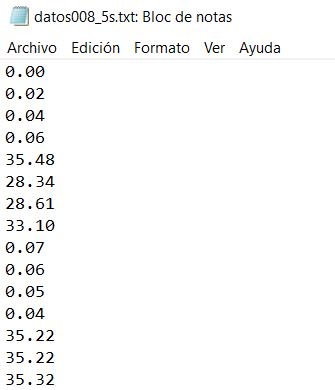
\includegraphics[scale=0.75]{images/salidaHMC5983C.png}
\caption [Archivo de salida código C del sensor HMC5983]{Archivo de salida creado por el código programado en C que lanza el sensor HMC5983}%
\label{fig:salidaHMCC}
\end{figure}


\subsection{Configuración sensor HC-SR04}

El segundo prototipo se creará utilizando un sensor ultrasónico HC-SR04, las características de este sensor están descritas en la sección correspondiente al mismo. 

Partiendo de la base inicial, el primer paso será realizar las conexiones del sensor a los pines GPIO de la placa R-Pi, para crear este enlace necesitamos conectar los cuatro de los pines del sensor; vcc (positivo), GND (negativo), echo (receptor de señales) y Trig (transmisor de señales). Estos pines serán conectados a la placa R-Pi de la siguiente manera:
\begin{itemize}
    \item \textbf{VCC}: 5V - PIN 2
    \item \textbf{GNC}: Negativo - PIN 6
    \item \textbf{Trig}: GPIO 17 - PIN 11
    \item \textbf{Echo}: GPIO 27 - PIN 13
\end{itemize}
Como puede observarse en el diagrama de conexiones de la Figura~\ref{fig:diagramaConexionesHC}, la conexión del sensor tiene la peculiaridad de necesitar usar dos resistencias: una de 330 \(\Omega\) y otra de 470 \(\Omega\), esto se debe a que los pines GPIO toleran un máximo de 3.3V y el sensor debe conectarse a 5V. En nuestro caso utilizaremos de manera similar dos resistencias: una de 1k\(\Omega\) y otra de 2.2k\(\Omega\)


\begin{figure}[h]
\centering
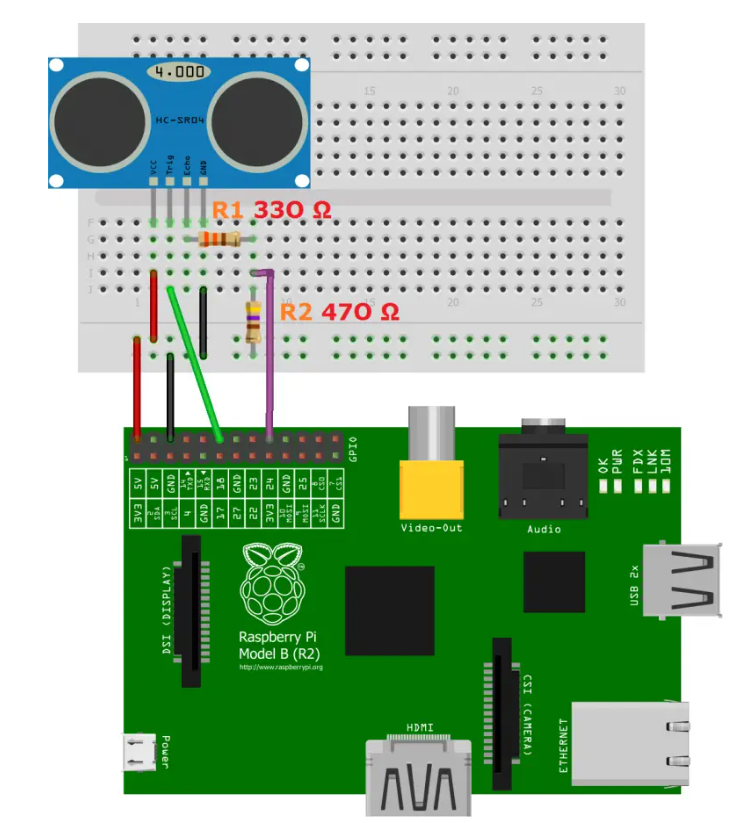
\includegraphics[scale=0.65]{images/conexionRaspHCSR04.png}
\caption[Conexión HC-SR04 a Raspbery-Pi]{Diagrama de conexiones del sensor HC-SR04 a raspberry-Pi 3.}%
\label{fig:diagramaConexionesHC}
\end{figure}

Una vez creada la conexión, se puede comenzar a crear el código que recibirá los datos del sensor. 

\newpage
\subsubsection{Código Python sensor HC-SR04}

El código Python de este sensor resulta bastante sencillo de implementar debido a la amplia cantidad de información que se encuentra al respecto en diversas páginas o manuales, a continuación se explican las partes más importantes del mismo. 

En el caso de Python utilizaremos la biblioteca RPi.GPIO que proporciona acceso directo a los pines GPIO de la placa R-Pi. Gracias a esta biblioteca podemos determinar el modo de numeración de los pines, en este caso que se establece como BCM(Broadcom SOC chanel) utilizando \textit{GPIO.setmode} y \textit{GPIO.setup}, esto nos permite determinar cuál es el pin de entrada (Echo (GPIO 27)) y cuál el de salida (Trig (GPIO17)).

El siguiente paso es crear la función que mide la distancia, esta establece el pin Trig en alto durante un corto periodo de tiempo para activar el pulso de disparo de ultrasonido del sensor y luego se espera un breve tiempo antes de establecer el mismo pin en bajo para finalizar el pulso. Registrando los tiempos de inicio y fin del pulso (pulse\_start y pulse\_end) se puede medir la duración del pulso ultrasónico reflejado, para ello se entra en un bucle mientras el pin ECHO esté en estado bajo, lo que indica que aún no se ha recibido el pulso ultrasónico reflejado. Durante este tiempo, se actualiza continuamente el valor de $pulse\_start$ con el tiempo actual hasta que se detecte el inicio del pulso reflejado.Después, se entra en otro bucle mientras el pin ECHO esté en estado alto, lo que indica que el pulso ultrasónico reflejado está siendo recibido. Se actualiza constantemente el valor de $pulse\_end$ con el tiempo actual hasta que se detecte el final del pulso reflejado.

Por último, se realiza el cálculo de la distancia utilizando el inicio y fin del pulso obtenido anteriormente. Este cálculo se basa en dividir la duración del puso entre dos y multiplicarlo por la velocidad del sonido del aire (aproximadamente 34000 cm/s). La distancia se calcula como la mitad del tiempo total de ida y vuelta del pulso, ya que el pulso viaja desde el sensor hasta el objeto y vuelve al sensor.

A través de este código obtenemos por terminal un bucle de datos de distancia, medida en centímetros, con un ratio que puede ser modificable estableciendo diferentes valores en el $time.sleep()$ del <<try>>. En la Figura~\ref{fig:salidaUltrasonidoP} se puede observar una salida de ejemplo. 

\begin{figure}[h]
\centering
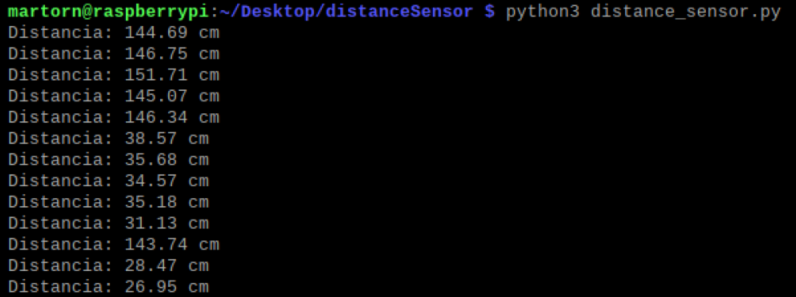
\includegraphics[scale=0.8]{images/salidaUltrasonidoPython.png}
\caption[Salida terminal del código Python del sensor HC-SR04]{Visualización de la salida del terminal de la placa R-Pi del código programado en Python que lanza el sensor HC-SR04.}%
\label{fig:salidaUltrasonidoP}
\end{figure}

\lstset{language=Python, breaklines=true, basicstyle=\footnotesize}
\begin{lstlisting}[frame=single]
import RPi.GPIO as GPIO
import time

GPIO.setmode(GPIO.BCM)

TRIG_PIN = 17
ECHO_PIN = 27

GPIO.setup(TRIG_PIN, GPIO.OUT)
GPIO.setup(ECHO_PIN, GPIO.IN)

def measure_distance():
    GPIO.output(TRIG_PIN, True)
    time.sleep(0.00001)
    GPIO.output(TRIG_PIN, False)

    pulse_start = time.time()
    pulse_end = time.time()
    
    while GPIO.input(ECHO_PIN) == 0:
        pulse_start = time.time()

    while GPIO.input(ECHO_PIN) == 1:
        pulse_end = time.time()

    pulse_duration = pulse_end - pulse_start
    distance = pulse_duration * 34300 / 2

    return round(distance, 2)  # Redondear la distancia a 2 decimales

try:
    while True:
        dist = measure_distance()
        print("Distancia:", dist, "cm")
        time.sleep(0.5)

except KeyboardInterrupt:
    print("Programa interrumpido por el usuario")

finally:
    GPIO.cleanup()
\end{lstlisting}

\subsubsection{Código C del sensor HC-SR04}

El código C utilizado para la lectura de distancia del sensor ultrasónico se ha basado en el funcionamiento del código Python ya que la lectura de este tipo de sensores no suele implementarse en este lenguaje. A diferencia del código anterior, la biblioteca principal utilizada para acceder a los pines GPIO será \textit{wiringPi}. Otra diferencia es que en este código se ha implementado la funcionalidad de poder modificar el tiempo y el ratio de lectura, y además los datos serán guardados en un archivo de texto para que puedan ser visualizados desde el servidor.

La manera de implementar la lectura es similar al código Python. En primer lugar, es importante definir qué pines representarán TRIG y ECHO para posteriormente configurar TRIG como salida y ECHO como entrada mediante el comando \textit{wiringPiSetupGpio()}. El siguiente paso es, al igual que en el código Python, activar el pulso de disparo enviando un pulso corto al pin TRIG, medir el <<tiempo de vuelo>> del pulso (tiempo entre activación y recepción del eco) y realizar el cálculo pertinente para convertir el tiempo en distancia.

Además, en este código se introduce la posibilidad de que el eco del pulso no se detecte o este sea demasiado largo para que esos valores no sean almacenados ya que no son útiles.

Por último, nos encontramos con la función principal \textit{main()}, que se ocupa de que lo siguiente:
\begin{itemize}
    \item  Verificar que los argumentos necesarios sean introducidos correctamente, en este caso dos: el tiempo de lectura y el ratio de lectura.
    \item Llamar a la función que configura los pines GPIO, denominada \textit{setup()}.
    \item Abrir un archivo en modo lectura en el que se escribirán los datos obtenidos por el sensor
    \item Crear un bucle de recogida de datos que se ejecute hasta que se alcance el tiempo especificado por el argumento introducido anteriormente. En cada iteración se llama a la función que obtiene la distancia y se almacena el dato obtenido en el archivo abierto.
    \item Controlar la frecuencia de lectura de datos utilizando \textit{time\_sleep()} con el argumento introducido.
\end{itemize}
\clearpage

\lstset{language=C, breaklines=true, basicstyle=\footnotesize}
\begin{lstlisting}[frame=single]
#include <stdio.h>
#include <stdlib.h>
#include <wiringPi.h>
#include <unistd.h>
#include <math.h>
#include <time.h>
#include <pigpio.h>


#define TRIG_PIN 17 //Trig conectado a GPIO17
#define ECHO_PIN 27 //Echo conectado a GPIO27

void setup() {
    wiringPiSetupGpio();
    pinMode(TRIG_PIN, OUTPUT);
    pinMode(ECHO_PIN, INPUT);
}

void time_sleep(double seconds) {
    struct timespec req;
    req.tv_sec = (time_t)seconds;
    req.tv_nsec = (long)((seconds - (time_t)seconds) * 1e9);

    while (nanosleep(&req, &req) == -1) {
        continue;
    }
}

float getDistance() {
    digitalWrite(TRIG_PIN, LOW);
    delayMicroseconds(2); //2ms delay

    digitalWrite(TRIG_PIN, HIGH);
    delayMicroseconds(10); //10 ms delay
    digitalWrite(TRIG_PIN, LOW);

    unsigned int timeout = 50000; // 50 ms en caso de no ser detectado
    unsigned int start_time, end_time;
    float distance;

    start_time = micros();

    while (digitalRead(ECHO_PIN) == LOW) {
        if ((micros() - start_time) > timeout) {
            printf("Error: No se detecto el pulso de eco.\n");
            return -1.0;
        }
    }

    start_time = micros();

    while (digitalRead(ECHO_PIN) == HIGH) {
        if ((micros() - start_time) > timeout) {
            printf("Error: Pulso de eco demasiado largo.\n");
            return -1.0;
        }
        end_time = micros();
    }

    float pulse_duration = (float)(end_time - start_time);
    distance = pulse_duration * 0.0343 / 2.0; // Calculo para pasar de tiempo a distancia

    return distance;
}

int main(int argc, char *argv[])
{
    if(argc !=3){
        printf("Uso:sudo %s [tiempo_lectura (segundos)] [ratio_lectura(segundos)]\n", argv[0]);
        return 1;
    }

    double tiempo = atof(argv[1]);
    double ratio = atof(argv[2]);
    setup();
    FILE *fp;
    fp = fopen("/home/martorn/Desktop/hello_erlang/src/sensorData/distancias.txt", "w"); // Modo escritura
    if (fp == NULL) {
        printf("Error al abrir el archivo para escritura.\n");
        return 1;
    }

    time_t start = time(NULL); // Obtener el tiempo de inicio
    time_t current_time;

    printf("Recogida de datos en curso");
    int cont=0;
    while (1) {
        float distance = getDistance();
        if (distance >= 0.0) {
            fprintf(fp,"%.2f \n",distance);
        }
        // Obtener el tiempo actual y comprobar si ha pasado el periodo de tiempo determinado de lectura de datos
        current_time = time(NULL);
        if (current_time - start >= tiempo) {
            break; // Salir del bucle despues de escribir durante el periodo de tiempo
        }
        for (int i=0; i<cont %4; i++){// FRECUENCIA DE LECTURA
            printf(".");
            }
        fflush(stdout);
        cont++;
        time_sleep(ratio); // Velocidad de lectura de los datos, periodo entre lectura y lectura.
    }
    printf("OK");

    return 0;
}
\end{lstlisting}

A la hora de compilar el código C, antes de ejecutarlo, es importante enlazar la \textit{wiringPi} (Controladora de pines GPIO) , para ello se debe ejecutar el comando de compilación \textit{gcc} añadiendo \textit{-lwiringPi}  como sigue:\\
\begin{lstlisting}[style=terminal]
gcc -o nombreEjecutable nombrePrograma.c -lwiringPi
\end{lstlisting}

En la Figura~\ref{fig:salidaUltrasonidoC} puede observarse el contenido del archivo creado por el programa anterior en el que aparecen los datos obtenidos por el sensor durante el periodo de lectura determinado.

\begin{figure}[h]
\centering
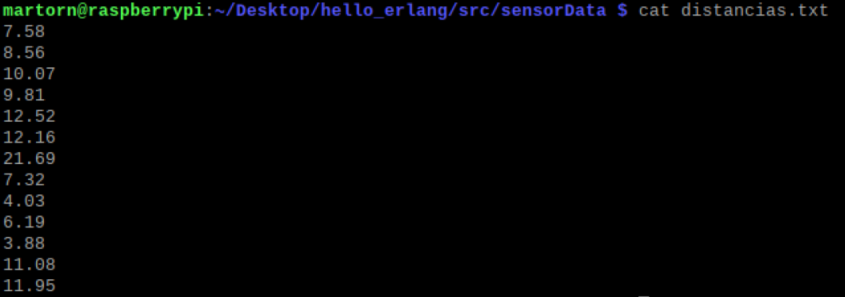
\includegraphics[scale=0.8]{images/salidaUltrasonidoC.png}
\caption[Salida de terminal del código C del sensor HC-SR04]{Visualización de la salida del terminal de la placa R-Pi del archivo creado por el código programado en C que lanza el sensor HC-SR04.}%
\label{fig:salidaUltrasonidoC}
\end{figure}


\section{Pruebas de frecuencia de lectura}

El HMC5983 es un magnetómetro de tres ejes que se comunica a través de una interfaz I2C, por lo que para modificar la frecuencia de lectura del sensor se deben utilizar comandos I2C.

Para cambiar la frecuencia de lectura del HMC5983, se debe configurar el registro de control de configuración (0x00). En este registro, los bits 5-2 controlan la tasa de datos, la cual se puede configurar entre los valores del 0 al 7. La frecuencia de muestreo más alta posible en el caso de este sensor es de 75 Hz por lo que será a la frecuencia a la que con configuraremos para que trabaje en su máximo rendimiento.

Con el comando: 
\begin{lstlisting}[style=terminal]
sudo i2cset -y 1 0x1E 0x00 [valor] 
\end{lstlisting}

Donde valor es el valor de configuración deseado en hexadecimal. Por ejemplo, para configurar una tasa de datos de 75 Hz, el valor se debe establecer en 0x70:

\begin{lstlisting}[style=terminal]
sudo i2cset -y 1 0x1E 0x00 0x70  
\end{lstlisting}


Mediante el comando anterior ya tenemos configurado el sensor para que lea datos en su máxima frecuencia disponible.\\

Al configurar la frecuencia en 75Hz conseguimos que el sensor obtenga una frecuencia de salida de datos de 75 por segundo, esto significa que el sensor proporcionará una nueva medición cada 1/75 segundos o 0.0133 segundos (aproximadamente cada 13 milisegundos), realmente el sensor tiene tres modos de uso; bajo, medio y alto (220 hz) pero para el uso del modo de alta frecuencia es necesario incluir resistencias. Se puede obtener también datos de temperatura del sensor a través de las direcciones 0x31 y 0x32 por si fuera necesario, en este caso no las utilizaremos. Todos estos datos se obtienen del datasheet del sensor.

El siguiente paso es comprobar si esa frecuencia de lectura es posible y nuestro programa C es capaz de leer a una velocidad igual o superior, para plantearnos esta situación debemos observar a qué frecuencia de lectura los datos comienzan a repetirse, en este punto existen dos posibilidades; que la frecuencia de lectura del código C sea superior a la que el sensor lee datos o que el código no sea suficientemente rápido como para leer a la frecuencia máxima del sensor.

A continuación, se realizaron varias pruebas a la frecuencia máxima del sensor modificando el ratio y el tiempo de lectura para observar si los datos comienzan a repetirse o el programa es capaz de almacenar todos los datos obtenidos por el sensor (tablas de los Cuadros \ref{tab:pf005}, \ref{tab:pf01} y \ref{tab:pf008}), durante las cuales se ha movido el sensor de manera aleatoria (movimientos de mano y muñeca) para que este vaya captando diferentes grados de cabeceo.


\begin{table}[htbp]
  \centering
  {\sffamily\small
  \begin{tabular}{|*{10}{r|}}
        \hline
    \multicolumn{10}{c}{\textbf{Prueba de frecuencia 1}: Medidas de ángulo de cabeceo (grados).}\\
    \hline
    35.25 & 35.25 & 35.26 & 35.26 & 35.25 & 45.00 & 45.00 & 44.98 & 44.97 & 44.98\\
    \hline
    44.98 & 44.98 & 35.25 & 35.28 & 35.27 & 35.27 & 35.26 & 35.25 & 35.24 & 35.22 \\
    \hline
    35.22 & 0.02 & 0.02 & 0.02 & 0.02 & 0.02 & 0.02 & 0.02 & 9.98 & 9.98\\
    \hline
    7.85 & 6.07 & 6.60 & 44.91 & 44.91 & 44.93 & 44.94 & 44.94 & 44.94 & 44.95 \\
    \hline
    44.95 & 59.33 & 59.33 & 45.04 & 18.93 & 45.07 & 45.07 & 11.3 & 11.3 & 11.3 \\
    \hline
  \end{tabular}
  } % fin de cambio de font
  \caption[Prueba de frecuencia 1] {50 primeros datos obtenidos del sensor HMC5983 tras realizar la prueba con una frecuencia de lectura de 0.05 segundos durante 5 segundos}\label{tab:pf005}
\end{table}

\begin{table}[htbp]
  \centering
  {\sffamily\small
  \begin{tabular}{|*{10}{r|}}
        \hline
    \multicolumn{10}{c}{\textbf{Prueba de frecuencia 2}: Medidas de ángulo de cabeceo (grados).}\\
    \hline
    0.05 & 0.04 & 6.22 & 8.43 & 8.32 & 10.61 & 10.30 &  35.30 & 35.29 & 12.29\\
    \hline
    15.29 & 33.35 & 35.34 & 35.35 & 44.96 & 44.97 & 46.47 & 46.95 & 48.93 & 48.92 \\
    \hline
    42.78 & 39.91 & 9.73 & 11.87 & 1.08 & 45.05 & 47.05 & 49.06 & 53.08 & 53.11 \\
    \hline
    35.29 & 33.48 & 31.19 & 30.32 & 0.01 & 0.02 & 0.80 & 3.16 & 15.22 & 18.34\\
    \hline
    18.60 & 35.32 & 33.87 & 31.28 & 29.14 & 18.37 & 21.56 & 6.58 & 43.56 & 48.47\\
    \hline
  \end{tabular}
  } % fin de cambio de font
  \caption[Prueba de frecuencia 2]{50 primeros datos obtenidos del sensor HMC5983 tras realizar la prueba con una frecuencia de lectura de 0.08 segundos durante 5 segundos}\label{tab:pf008}
\end{table}

\begin{table}[htbp]
  \centering
  {\sffamily\small
  \begin{tabular}{|*{10}{r|}}
      \hline
    \multicolumn{10}{c}{\textbf{Prueba de frecuencia 3}: Medidas de ángulo de cabeceo (grados).}\\
    \hline
    35.22 & 0.06 & 0.05 & 3.08 & 5.78 & 49.31 & 0.20 & 0.20 & 35.24 & 15.22 \\
    \hline
    17.30 & 35.33 & 31.60 & 31.30 & 35.29 & 45.98 & 55.30 & 58.32 & 40.97 & 44.98\\
    \hline
    44.99 & 41.58 & 0.11 & 0.09 & 3.06 & 5.02 & 25.30 & 35.28 & 39.78 & 35.22\\
    \hline
    33.91 & 31.20 & 35.25 & 34.19 & 29.23 & 35.28 & 39.30 & 44.97 & 46.76 & 44.13\\
    \hline
    41.89 & 35.22 & 37.9 & 35.30 & 11.33 & 8.30 & 2.25 & 1.33 & 6.89 & 7.47\\
    \hline
  \end{tabular}
  } % fin de cambio de font
  \caption[Prueba de frecuencia 3]{50 primeros datos obtenidos del sensor HMC5983 tras realizar la prueba con una frecuencia de lectura de 0.1 segundos durante 5 segundos}\label{tab:pf01}
\end{table}

\clearpage

En la \textbf{prueba de frecuencia 1} se han obtenido 100 datos, de los cuales, los 50 primeros se muestran en la tabla del Cuadro~\ref{tab:pf005}, en ella puede observarse como estos datos se repiten de manera continuada hasta en grupos de 7 elementos, esto denota que el programa está almacenando más datos de los que el sensor puede registrar, es por ello que cuando el programa solicita un dato nuevo este recoge el mismo que el recibido anteriormente.

En la \textbf{prueba de frecuencia 2} se han obtenido 62 datos de los que analizaremos los 50 primeros que se muestran en la tabla del Cuadro~\ref{tab:pf008}, como podemos ver en este caso los datos son diferentes entre sí y varían de forma progresiva sin saltos de ángulo demasiado pronunciados. 

Por último, en la tabla del Cuadro~\ref{tab:pf01} se muestran los 50 datos obtenidos durante la \textbf{prueba de frecuencia 3}, en este caso el ratio de lectura ha sido mucho más lento que en la prueba anterior, al ser un ratio de lectura menor, se han obtenido menos datos pero estos son siempre diferentes entre sí con saltos más significativos que en el caso de la prueba de frecuencia 2. Esto puede ser porque el sensor está leyendo a una frecuencia superior al programa y por tanto se están perdiendo datos.

En conclusión, una frecuencia de lectura óptima sería la utilizada en la prueba de frecuencia 2 (ratio=0.08 segundos) ya que en ella los datos no aparecen tan repetidos como en la prueba de frecuencia 1 y a su vez se obtienen muchos más datos válidos que en la prueba de frecuencia 3.

\chapter{Prototipo Incremental}

En el siguiente capítulo se describirá la implementación del segundo prototipo del sistema, el prototipo incremental. En este capítulo se incluirán los pasos necesarios para instalar la última versión de Erlang OTP sobre Easpberry-Pi así como versiones anteriores y se realizarán pruebas con este lenguaje para analizar su comportamiento sobre este sistema.

\section{Instalación de Erlang sobre Raspberry-Pi}
La instalación de Erlang en la placa R-Pi es sencilla y está más que probada ya que el sistema operativo Raspbian está basado en Debian. Podemos encontrar multitud de manuales de cómo hacerlo y en el caso de este proyecto se ha decidido utilizar \textit{Raspbian snap} para su instalación a través de terminal de texto.

Primero debe instalarse <<snapd>>, reiniciar la placa R-Pi e instalar core snap para obtener la última versión de snapd:
\begin{lstlisting}[style=terminal]
$ sudo apt update
$ sudo apt install snapd
$ sudo reboot
$ sudo snap install core
\end{lstlisting}

Por último, se instala Erlang/OTP mediante el siguiente comando:
\begin{lstlisting}[style=terminal]
$ sudo snap install erlang --classic
\end{lstlisting}

Tras realizar estos pasos ya disponemos de la última versión de Erlang disponible para la placa R-Pi con Raspbian, si ejecutamos el comando siguiente podemos acceder a la consola de Erlang donde veremos su versión y podremos ejecutar nuestros módulos, puede observarse su salida en el código de la Figura~\ref{fig:erlangRasp}.

\begin{lstlisting}[style=terminal]
$ erl
\end{lstlisting}

\begin{figure}[h]
\centering
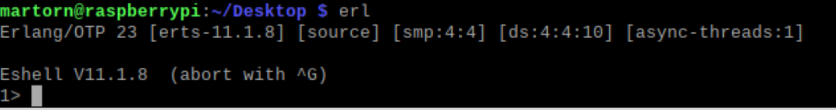
\includegraphics[scale=0.8]{images/erlangRaspberry.png}
\caption[Primer acceso a Erlang en Raspberry-Pi]{Visualización del terminal de la placa R-Pi al realizar el primer acceso a Erlang, puede visualizarse la versión del mismo.}%
\label{fig:erlangRasp}
\end{figure}


Puede darse el caso de necesitar alguna versión anterior de Erlang ya que alguna de las herramientas a utilizar no sea compatible con la última, si se desea instalar alguna versión específica de Erlang en la placa R-Pi deben de seguirse los siguientes pasos:

Primero debe actualizarse el sistema e instalar las dependencias que Erlang necesita para funcionar en este tipo de instalaciones:\\
 
\begin{lstlisting}[style=terminal]
$ sudo apt update
$ sudo apt upgrade
$ sudo apt install build-essential libncurses5-dev openssl libssl-dev fop xsltproc unixodbc-dev
\end{lstlisting}

Una vez realizado este paso debemos encontrar la versión deseada en el sitio Web oficial de descargas de Erlang \cite{erlang.orgStart}, es importante elegir correctamente una versión que sea compatible con la arquitectura de la placa R-Pi como puede ser armhf o arm64.

Tras la elección de la versión procedemos a descargarla y descomprimirla ya sea desde la página o desde terminal ejecutando los siguientes comandos:\\

\begin{lstlisting}[style=terminal]
$ wget https://erlang.org/download/otp_src_24.0.tar.gz
$ tar -xf otp_src_24.0.tar.gz
\end{lstlisting}

Por último, debemos acceder al directorio en el que se ha descomprimido el archivo y realizar la instalación de la siguiente manera:\\

\begin{lstlisting}[style=terminal]
$ cd otp_src_24.0
$ ./configure
$ make
$ sudo make install
\end{lstlisting}

Siguiendo los pasos anteriores podemos realizar en la placa R-Pi cualquier instalación de alguna versión Erlang que sea compatible con la misma.

\section{Pruebas con Erlang}

Para finalizar con este capítulo se ha creado un programa en Erlang para poner a prueba el rendimiento de este lenguaje sobre la placa R-Pi y su correcto funcionamiento, a su vez se ha creado un programa en Python con igual funcionalidad. El programa realiza una operación muy sencilla, calcula la suma de los primeros N números naturales y muestra el resultado, por último, para valorar el tiempo que tarda en realizar esta operación se muestra el tiempo de ejecución del programa en microsegundos. 

En el siguiente listado (tiempoEjecucion.erl) se muestra el código Erlang creado y la salida de tiempo obtenida realizando operaciones con $N$ números diferentes (Figura~\ref{fig:pruebaErlang} con $N=100$ y Figura~\ref{fig:pruebaErlang100000} con $N=100000$).\\

\lstset{language=Erlang, breaklines=true, basicstyle=\sffamily\footnotesize}
\begin{lstlisting}[frame=single, caption=tiempoEjecucion.erl]

-module(tiempoEjecucion).
-export([sum/1]).

sum(N) ->
    Start = os:timestamp(),
    Result = lists:sum(lists:seq(1, N)),
    End = os:timestamp(),
    Time = timer:now_diff(End, Start),
    io:format("La suma es ~p~n", [Result]),
    io:format("Tiempo de ejecucion: ~p microsegundos~n", [Time]).
\end{lstlisting}

\begin{figure}[h]
\centering
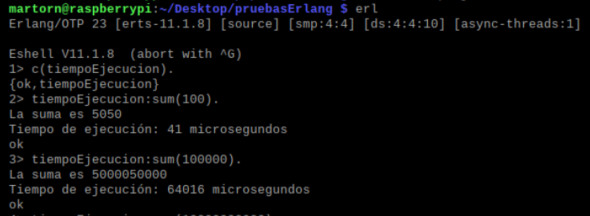
\includegraphics[scale=1.3]{images/pruebaErlang.png}
\caption[Salida de terminal suma de N=100 con Erlang]{Visualización de la salida de terminal de la placa R-Pi al ejecutar el programa que hace la suma de N en Erlang con N=100.}%
\label{fig:pruebaErlang}
\end{figure}

\begin{figure}[h]
\centering
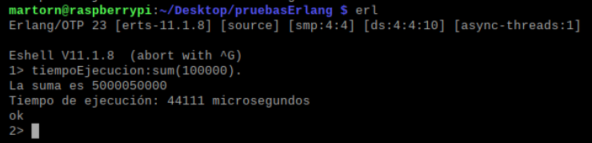
\includegraphics[scale=1.3]{images/pruebaErlang100000.png}
\caption[Salida de terminal suma de N=100000 con Erlang]{Visualización de la salida de terminal de la placa R-Pi al ejecutar el programa que hace la suma de N en Erlang con N=100000.}%
\label{fig:pruebaErlang100000}
\end{figure}

\clearpage
El siguiente código Python (tiempoEjecucion.py) tiene la misma funcionalidad que el código Erlang anterior, en la Figura~\ref{fig:pruebaPython} y Figura~\ref{fig:pruebaPython100000} pueden observarse las salidas obtenidas por el programa con los valores 100 y 100000 de N respectivamente.


\lstset{language=Python, breaklines=true, basicstyle=\footnotesize}
\begin{lstlisting}[frame=single, caption=tiempoEjecucion.py]
import time

def sum_numbers(n):
    start = time.time()
    result = sum(range(1, n+1))
    end = time.time()
    elapsed_time = (end - start) * 1000000
    print(f "La suma es {result}")
    print(f "Tiempo de ejecucion: {elapsed_time:.2f} microsegundos")

n = int(input("Ingrese el valor de N: "))
sum_numbers(n)
\end{lstlisting}

\begin{figure}[h]
\centering
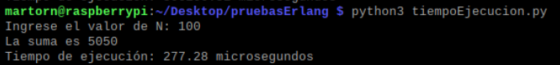
\includegraphics[scale=1.3]{images/pruebaPython100.png}
\caption[Salida de terminal suma de N=100 con Python]{Visualización de la salida de terminal de la placa R-Pi al ejecutar el programa que hace la suma de N en Python con N=100.}%
\label{fig:pruebaPython}
\end{figure}

\begin{figure}[h]
\centering
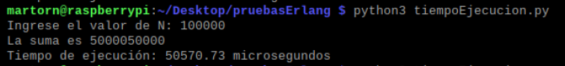
\includegraphics[scale=1.3]{images/pruebaPython.png}
\caption[Salida de terminal suma de N=100000 con Erlang]{Visualización de la salida de terminal de la placa R-Pi al ejecutar el programa que hace la suma de N en Python con N=100000.}%
\label{fig:pruebaPython100000}
\end{figure}

Los resultados se muestran en la tabla del Cuadro~\ref{tab:tiempos1}. Puede verse que el programa creado en Erlang es algo más rápido que el programado en Python pero es una diferencia muy poco significativa. Por otro lado, el código C es algo más rápido que ambos. De cualquier manera, vemos que Erlang parece plenamente funcional en la placa R-Pi y que su rendimiento es similar al de Python, lenguaje mucho más frecuente en este tipo de dispositivos. Para obtener conclusiones más precisas sobre las velocidades de cada lenguaje sería conveniente realizar muchas más pruebas o ejecuciones con diferentes repeticiones. 

\begin{table}[h]
\begin{center}
\sffamily
\begin{tabular}{lcc}
\toprule[1,7pt]
%\begin{tabular}{|>{\columncolor{gray!20}}lcc|}\hline
     &  \multicolumn{2}{c}{Tiempo invertido (µs).} \\
     \cline{2-3}
%\rowcolor{gray!20}
Lenguaje & 100 repeticiones & 100,000 repeticiones \\
\midrule[1.2pt]
Erlang & 41 & 44111 \\
\hline
Python & 277 & 50570 \\
\hline
C & 28 & 39587 \\
\bottomrule[1,7pt]
\end{tabular}
\caption[Comparativa de tiempos de ejecución]{Comparativa de tiempos de ejecución entre Erlang, Python y C medido en microsegundos realizando 100 y 100000 repeticiones.}%
\label{tab:tiempos1}
\end{center}
\end{table}







 

\chapter{Prototipo Funcional}

En este capítulo se describe el último prototipo del proyecto, el prototipo funcional. En él se expone todo lo referente a la implementación del servidor Erlang sobre la placa R-Pi, esto incluye: la creación del servidor base, la implementación de un servicio API REST, la creación de la interfaz del servidor y la implementación de la funcionalidad de lanzar la lectura de los sensores. Por último, se realizan pruebas de carga sobre el servidor para poner a prueba su rendimiento.

\section{Elección del servidor Web}

Existen múltiples opciones para crear servidores web usando Erlang, a continuación se describen algunos de los más comúnmente usados:
\begin{enumerate}
    \item \textbf{Yaws}: Es uno de los servidores web más populares en el entorno de Erlang y se destaca por su eficiencia y escalabilidad.
    \item \textbf{Cowboy}: Servidor web escrito en Erlang que ofrece un enfoque ligero y eficiente para el manejo de solicitudes HTTP. Es conocido por su rendimiento y flexibilidad, y se utiliza ampliamente en el desarrollo de aplicaciones web en Erlang.
    \item \textbf{MongooseIM}: Servidor de mensajería instantánea y chat en tiempo real. Está basado en el protocolo XMPP (Extensible Messaging and Presence Protocol) y ofrece capacidades de mensajería escalables y confiables.
    \item \textbf{RabbitMQ}: Servidor de mensajes y cola de tareas. Proporciona un sistema de mensajería robusto y escalable para el intercambio de datos entre diferentes componentes de una aplicación.
\end{enumerate}

A su vez existen bibliotecas y herramientas incluidas en el propio lenguaje como puede ser \textit{inets}, que proporciona una amplia gama de funcionalidades relacionadas con la infraestructura web y facilita el desarrollo de aplicaciones HTTP y otros protocolos web.

Debido a la naturaleza de este proyecto se ha decidido utilizar \textbf{Cowboy} ya que se trata de un servidor sencillo de usar y eficiente para este tipo de tareas, además es un servidor que soporta varios protocolos web como HTTP y WebSoquets y proporciona un sistema de enrutamiento flexible que permite asociar patrones de URL con funciones específicas, lo que será utilizado posteriormente para la funcionalidad de API REST . Para comenzar, se han seguido los pasos de instalación y creación de este tipo de servidores que nos ofrece la página oficial en su apartado <<Getting started>>, mediante estos podremos crear la base desde donde avanzar hacia el objetivo final de nuestro servidor funcional.

Un servidor Cowboy funciona siguiendo un modelo de concurrencia basado en actores y utiliza el sistema de concurrencia ligera de Erlang para manejar conexiones concurrentes de manera eficiente. A continuación, se explica de manera general como funciona:

\begin{enumerate}
    \item \textbf{Configuración}: En primer lugar, se realiza la configuración de Cowboy. Esto implica definir los puertos en los que el servidor escuchará las solicitudes entrantes, configurar enrutamiento y asociar funciones o módulos a rutas específicas.
    \item \textbf{Recepción de solicitudes}: Una vez que el servidor está configurado y en ejecución, comienza a escuchar las solicitudes entrantes en los puertos especificados. Cuando se recibe una solicitud HTTP, Cowboy la captura y la enruta a la función o módulo correspondiente según las reglas de enrutamiento definidas.
    \item \textbf{Enrutamiento}: Como se comentó anteriormente, Cowboy utiliza un sistema de enrutamiento flexible que permite asociar patrones de URL con funciones o módulos específicos. Esto se puede hacer mediante el uso de patrones de coincidencia o mediante la configuración manual de las rutas. Al recibir una solicitud, Cowboy verifica la ruta solicitada y la redirige a la función o módulo apropiado para su procesamiento.
    \item \textbf{Procesamiento de la solicitud}: Una vez que Cowboy ha determinado la función o módulo encargado de procesar la solicitud, pasa los datos de la solicitud (como los encabezados, el cuerpo y los parámetros) a dicha función o módulo. Aquí es donde se realiza la lógica de la aplicación para procesar la solicitud y generar una respuesta, en nuestro caso ejecutar un sensor, devolver datos o mostrar descripciones.
    \item \textbf{Generación de la respuesta}: La función o módulo encargado de procesar la solicitud en Cowboy genera una respuesta apropiada. Esto puede implicar la generación de contenido dinámico, la consulta de una base de datos o cualquier otra operación necesaria para construir la respuesta HTTP adecuada.
    \item \textbf{Envío de la respuesta}: Una vez generada la respuesta, Cowboy envía la respuesta HTTP al cliente que realizó la solicitud. Esto incluye enviar los encabezados HTTP adecuados y el cuerpo de la respuesta si corresponde.
\end{enumerate}

Este proceso se repite para cada solicitud entrante que recibe Cowboy. El servidor está diseñado para manejar múltiples solicitudes concurrentemente utilizando el modelo de concurrencia de Erlang y aprovechando la escalabilidad y eficiencia inherentes al lenguaje.

\cleardoublepage


\section{Creación del servidor Web}

\subsection{Objetivos de funcionalidad}

Tras el análisis de requisitos del proyecto se ha decidido crear un servidor que disponga de cierta funcionalidad y que esta sea fácilmente escalable, por ello se ha elegido el diseño de una API REST que, mediante la utilización de Cowboy, implementará un servidor que permita hacer lo siguiente:

\begin{enumerate}
    \item Acceso a una página de Inicio.
    \item Ver qué sensores se encuentran disponibles.
    \item Acceder a la descripción de cada uno de los sensores junto con su manual de uso.
    \item Lanzar la lectura de los sensores con valores por defecto.
    \item Lanzar la lectura de los sensores con la posibilidad de modificar sus argumentos de tiempo de lectura y ratio de lectura.
    \item Acceder a los archivos que almacenan los datos recibidos por los sensores.
\end{enumerate}

Los documentos que devolverá el servidor ya sean manuales o descripciones serán almacenadas en formato JSON. Los documentos que almacenan los datos de los sensores permanecerán en .txt.


\subsection{Configuración inicial}%
\label{sec:ConfigCowboy}

La configuración inicial del servidor Erlang implementado con Cowboy se realiza siguiendo los pasos de la sección <<Getting Started>> de la página ninenines.eu referenciada en \cite{Nines2012}. A continuación, se describirán los pasos seguidos para conseguir una pequeña aplicación de servidor que se utilizará como base desde la que avanzar hacia el objetivo final.

En primer lugar, debe crearse el directorio en el que almacenaremos nuestro servidor, para ello ejecutamos los siguientes comandos en el terminal de la placa R-Pi sobre el directorio en el que deseamos trabajar para crear el nuevo directorio y acceder a él.\\ 

\begin{lstlisting}[style=terminal]
$ mkdir hello_erlang
$ cd hello_erlang
\end{lstlisting}

El siguiente paso es realizar la descarga de Erlang.mk, esta herramienta proporcionará una forma simple de compilar, probar y gestionar dependencias para aplicaciones Erlang utilizando un enfoque basado en Makefile para definir el proceso de construcción y automatización de tareas comunes. Para descargar esta herramienta utilizaremos el comando\\

\begin{lstlisting}[style=terminal]
$ wget https://erlang.mk/erlang.mk
\end{lstlisting}

Tras realizar la descarga, se utiliza bootstrap para crear el entorno de la aplicación y su versión ejecutable con el comando siguiente.

\begin{lstlisting}[style=terminal]
make -f erlang.mk bootstrap bootstrap-rel
\end{lstlisting}

Una vez realizados estos pasos podemos construir y lanzar el servidor pero aún faltarán pasos para que este funcione correctamente.\\

La configuración de Cowboy comienza por modificar el Makefile para que el sistema detecte que vamos a usar los plugins y dependencias de Cowboy junto con su respectiva versión. El Makefile debe quedar de la siguiente manera:\\

\lstset{language=C, breaklines=true, basicstyle=\sffamily\footnotesize}
\begin{lstlisting}[frame=single]
PROJECT = hello_erlang

DEPS = cowboy
dep_cowboy_commit = 2.6.3

DEP_PLUGINS = cowboy
include erlang.mk
\end{lstlisting}

El siguiente paso es definir las rutas que Cowboy utilizará para enlazar con los módulos del servidor que realizarán las acciones, también llamados <<handlers>>, para ello se modifica el archivo hello\_erlang\_app.erl que se ha creado automáticamente en el directorio /src. En esta primera parte de la configuración únicamente le introduciremos la ruta raíz <</>> que se redirigirá a hello\_handler.erl, además se añade la configuración que lanzará el servidor en localhost sobre el puerto 8080, todo ello en la función start/2. El código de hello\_erlang\_app.erl quedaría como sigue:\\

\lstset{language=Erlang, breaklines=true, basicstyle=\sffamily\footnotesize}
\begin{lstlisting}[frame=single]
start(_Type, _Args) ->
    Dispatch = cowboy_router:compile([
        {'_', [{"/", hello_handler, []}]}
    ]),
    {ok, _} = cowboy:start_clear(my_http_listener,
        [{port, 8080}],
        #{env => #{dispatch => Dispatch}}
    ),
    hello_erlang_sup:start_link().
\end{lstlisting}

Por último, debe crearse el handler hello\_handler.erl que será quien responda a la llamada <</>> desde el servidor. Para esta configuración inicial únicamente debemos esperar una respuesta correcta por parte del servidor y que este devuelva <<Hello Erlang!>>. Para ello, se introducirá la siguiente función en hello\_handler.erl.\\

\lstset{language=Erlang, breaklines=true, basicstyle=\sffamily\footnotesize}
\begin{lstlisting}[frame=single]
init(Req0, State) ->
    Req = cowboy_req:reply(200,
        #{<<"content-type">> => <<"text/plain">>},
        <<"Hello Erlang!">>,
        Req0),
    {ok, Req, State}.
\end{lstlisting}

Tras estos pasos ya tenemos disponible el funcionamiento más básico del servidor Erlang utilizando Cowboy, a partir de aquí podremos ir añadiendo funcionalidad para que cumpla los requisitos del proyecto. En los siguientes apartados de esta sección se describirán los puntos principales del proceso de creación del mismo.

\subsection{Diseño de la API REST}

El esquema de la API REST será sencillo y se basará en carpetas como los sistemas operativos habituales. A continuación se describirá el diseño de la API utilizando un árbol de directorios.\\

\dirtree{%
.1 /.
.2 sensores.
.3 magnetómetro.
.4 launch.
.4 data.
.5 angulos.txt.
.3 ultrasonido.
.4 launch.
.4 data.
.5 distancias.txt.
}

A través de este esquema se puede observar el funcionamiento del servidor. En primer lugar, al acceder al él nos encontramos en la carpeta raíz, que nos mostrará una introducción al servidor y ofrecerá el acceso a la descripción de los sensores. En caso de acceder a la carpeta /sensores nos encontraremos con la descripción de las posibilidades de manejo del servidor sobre los diferentes sensores disponibles.

Tras elegir alguno de los sensores accediendo mediante su nombre (ej: /sensores/ultrasonido) dispondremos de una descripción detallada del mismo junto con un manual que describirá cómo ejecutar su lectura, ya sea de manera predeterminada o personalizada así como la forma de acceder a los datos obtenidos. Por último, el directorio <<../data>> nos permitirá visualizar al archivo txt que contendrá los últimos datos leídos por el sensor seleccionado.


\subsection{Descripción de sensores}

La descripción de los sensores y el manual de uso de la API REST se creará en lenguaje JSON, posteriormente, estos archivos serán referenciados desde el servidor para que sea el navegador quien los analice y los muestre en este formato.

Se han creado tres archivos JSON, uno para cada sensor utilizado y otro para la página que muestra las posibilidades de ejecución de los mismos. A continuación se muestra un ejemplo del archivo que se visuaizará en caso de acceder al directorio <</sensores>>, este ofrece un diagrama sobre las diferentes posibilidades de acceso desde este directorio.
\clearpage
\lstset{language=JSON, breaklines=true, basicstyle=\footnotesize}
\begin{lstlisting}[frame=single, caption=sensores.json]
{
  "sensores": [
    {
      "name": "Sensor Magnetometro HMC5983",
      "specs": "http://localhost:8080/sensores/magnetometro",
      "default_launch": "http://localhost:8080/sensores/magnetometro/launch",
      "custom_launch" : "http://localhost:8080/sensores/magnetometro/launch?time=X&frec=Y",
      "last_data" : "http://localhost:8080/sensores/magnetometro/data"
    },
    {
      "name": "Sensor de Distancia HJC-SR04",
      "specs": "http://localhost:8080/sensores/ultrasonido",
      "default_launch": "http://localhost:8080/sensores/ultrasonido/launch",
      "custom_launch" : "http://localhost:8080/sensores/ultrasonido/launch?time=X&frec=Y",
      "last_data" : "http://localhost:8080/sensores/ultrasonido/data"
    }
  ]
}
\end{lstlisting}


\subsection{Ejecución de sensores}

Los sensores deben poder ejecutarse desde el servidor, por ello se ha creado un módulo que se ocupa únicamente de realizar estas ejecuciones, se trata de launch\_handler.erl. En esta sección se describirá el código de este módulo.

En primer lugar, ha de tenerse en cuenta como se ejecutan los sensores para posteriormente tratar de realizar esta ejecución desde el servidor. Los sensores utilizan un código escrito en lenguaje C, descrito en el Capítulo~\ref{cap.prototipoExploracion}, este código necesita dos argumentos para ejecutarse y almacena los datos en un archivo .txt. 

El lugar de almacenamiento del código es la placa de desarrollo, al igual que los sensores que están conectados a la misma, por esto la tarea del servidor es ejecutar este código en la placa R-Pi pasándole los argumentos necesarios para que, al finalizar la ejecución, el servidor pueda acceder al archivo creado con los datos leídos por el sensor. A continuación se explicará detalladamente el funcionamiento del módulo Erlang creado para las tareas mencionadas. A este módulo se accederá al lanzar <<../launch>> desde el servidor eligiendo con anterioridad el tipo de sensor a lanzar.

En primer lugar, se realiza la exportación de las funciones a utilizar, se trata de  \textit{init/2}, \textit{execute\_ultrasonido/2}, \textit{execute\_magnetometro/2}, \textit{allowed\_methods/2} y \textit{content/2}. Estas funciones se encuentran descritas a continuación:

\begin{itemize}
    \item \textbf{init/2}: Encargada de inicializar la respuesta a una solicitud HTTP con un código de estado 200 y establecer el tipo de contenido como <<text/plain>>.
    \item \textbf{allowed\_methods/2}: Especifica los métodos HTTP permitidos para una solicitud determinada, en este caso GET, POST y DELETE.
    \item \textbf{content/2}: Se utiliza para procesar las solicitudes HTTP entrantes y determinar cómo responder. Dependiendo de la ruta y los parámetros de la consulta, se ejecutan las funciones correspondientes para lanzar la ejecución de los programas externos y recopilar datos de los sensores. En caso de no recibir parámetros se establecen por defecto, de esta manera cuando llega únicamente una petición de lanzamiento de un sensor sin especificar parámetros de lanzamiento, no ocurre un error sino que se llama a la función de ejecución del sensor con estos parámetros por defecto.
    \item \textbf{execute\_ultrasonido/2} : Responsable de la ejecución de los comandos externos mediante el uso de ports Erlang, esta función es llamada a través de \textit{content/2} cuando se recibe la solicitud\\ <</ultrasonido/launch>> y necesita los parámetros Time y Frec para realizar la ejecución del código que lanza la lectura del sensor. Por último, también llama a \textit{receive\_data}, que recibirá la respuesta del código ejecutado.

    \item \textbf{execute\_magnetometro/2} : Funciona de manera similar a \textit{execute\_ultrasonido/2} solo que esta ejecuta el código del sensor magnetómetro y es llamada cuando se recibe la solicitud\\ <</magnetometro/launch>>.
    
    \item \textbf{receive\_data/1}: Se encarga de recibir los datos enviados por los programas externos a través del port Erlang y realizar acciones específicas según los datos recibidos. Por ejemplo, muestra mensajes de éxito cuando los datos se han recopilado correctamente. Para saber que todo ha ido bien utiliza la última salida de los programas C como indicador de fin de ejecución.
\end{itemize}

   El uso de un port Erlang permite la comunicación y la interoperabilidad con programas escritos en otros lenguajes de programación, como es el caso de C. El uso de port es sencillo y consta de varios pasos:
   \begin{enumerate}
       \item Definir el comando o programa externo a ejecutar y determinar su ruta así como sus posibles argumentos.
       \item Abrir el port utilizando la función <<open\_port/2>>, esta función toma como argumento una tupla que especifica como se debe lanzar el programa externo, incluyendo el comando a ejecutar y cualquier opción adicional.
       \item Procesar los datos recibidos: Se utiliza la función \textit{receive} para recibir y procesar los datos enviados por el programa externo a través del port.
   \end{enumerate}

\lstset{language=Erlang, breaklines=true, basicstyle=\sffamily\footnotesize}
\begin{lstlisting}[frame=single, caption=launch\_handler.erl]
-module(launch_handler).

-export([
    init/2,
    execute_ultrasonido/2,
    execute_magnetometro/2,
    allowed_methods/2,
    content/2
]).

init(Req0, State) ->
    Req = cowboy_req:reply(200,
        #{<<"content-type">> => <<"text/plain">>},
        content(cowboy_req:path(Req0), cowboy_req:qs(Req0)),
        Req0),
    {ok, Req, State}.

allowed_methods(Req, State) ->
    Methods = [<<"GET">>, <<"POST">>, <<"DELETE">>],
    {Methods, Req, State}.
    
execute_ultrasonido(Time, Frec) ->
    Command = "/home/martorn/Desktop/distanceSensor/ultrasonido " ++ Time ++ " " ++ Frec,
    Port = open_port({spawn, Command}, [stream]),
    receive_data(Port).

execute_magnetometro(Time, Frec) ->
    Command = "sudo /home/martorn/Desktop/hmc5983_i2c/CabeceoArchivo/cabeceoArchivo " ++ Time ++ " " ++ Frec,
    Port = open_port({spawn, Command}, [stream]),
    receive_data(Port).

receive_data(Port) ->
    receive
        {Port, {data, Data}} when Data == "UltOK" -> % Utiliza "UltOK" como indicador de fin de ejecucion.
          "Recogida de datos finalizada correctamente!, accede al archivo a traves de http://localhost:8080/sensores/ultrasonido/data";
        
        {Port, {data, Data}} when Data == "MagOK" -> % Utiliza "MagOK" como indicador de fin de ejecucion.
        "Recogida de datos finalizada correctamente!, accede al archivo a traves de http://localhost:8080/sensores/magnetometro/data";
        
        {Port, {data, Data}} ->
		io:format("~p~n", [Data]),
            receive_data(Port);
        {Port, {error, Reason}} ->
		Reason,
            io:format("Error al recibir datos del programa C: ~p~n", [Reason])
        end.
    
content(Path, QueryString) when Path == <<"/sensores/ultrasonido/launch">> ->
	
	Params = cow_qs:parse_qs(QueryString), %Divide la parte del query en cada uno de sus argumentos
	io:format("Params: ~p~n", [Params]),
	TimeBin = proplists:get_value(<<"time">>, Params, <<"5">>), %Obtiene el valor de time en binario, formato <<"x">>
	FrecBin = proplists:get_value(<<"frec">>, Params, <<"0.5">>), %Obtiene el valor de frec en binario, formato <<"x">>
	Time = binary_to_list(TimeBin), %Pasa el argumento a list para que la funcion que ejecuta el codido pueda leerlo
	Frec = binary_to_list(FrecBin),
	io:format("Time: ~p~n", [Time]),
	io:format("Frec: ~p~n", [Frec]),
    execute_ultrasonido(Time, Frec); %Se lanza la funcion con los argumentos especificados
		
	
content(Path, QueryString) when Path == <<"/sensores/magnetometro/launch">> ->
	
	Params = cow_qs:parse_qs(QueryString), %Divide la parte del query en cada uno de sus argumentos
	io:format("Params: ~p~n", [Params]),
	TimeBin = proplists:get_value(<<"time">>, Params, <<"5">>), %Obtiene el valor de time en binario, formato <<"x">>
	FrecBin = proplists:get_value(<<"frec">>, Params, <<"0.5">>), %Obtiene el valor de frec en binario, formato <<"x">>
	Time = binary_to_list(TimeBin), %Pasa el argumento a tipo list para que la funcion que ejecuta el codido pueda leerlo
	Frec = binary_to_list(FrecBin),
	io:format("Time: ~p~n", [Time]),
	io:format("Frec: ~p~n", [Frec]),
    execute_magnetometro(Time, Frec); %Se lanza la funcion con los argumentos especificados
  
content(_, _) ->
    <<"Not Found">>.
\end{lstlisting}

\subsection{Muestra de datos}

La visualización de los datos leídos por cada uno de los sensores la realiza el módulo data\_handler.erl que es llamado desde hello\_erlang\_app.erl cuando se realiza la solicitud HTTP con la dirección\\ <</sensores/SensorX/data>>. Su código es sencillo, cuando llega una solicitud a este módulo determina de qué sensor se trata y realiza la lectura del archivo creado por este sensor, el cual se almacena en una ubicación específica de la placa R-Pi. \\

\lstset{language=Erlang, breaklines=true, basicstyle=\sffamily\footnotesize}
\begin{lstlisting}[frame=single, caption=data\_handler.erl]

-module(data_handler).

-export([
    init/2,
    allowed_methods/2,
    content/2
]).

init(Req0, State) ->
    Req = cowboy_req:reply(200,
        #{<<"content-type">> => <<"text/plain">>},
        content(cowboy_req:path(Req0), cowboy_req:qs(Req0)),
        Req0),
    {ok, Req, State}.

allowed_methods(Req, State) ->
    Methods = [<<"GET">>, <<"POST">>, <<"DELETE">>],
    {Methods, Req, State}.
    
content(Path, _) when Path == <<"/sensores/ultrasonido/data">> -> 
     {ok, Data} = file:read_file("/home/martorn/Desktop/hello_erlang/src/sensorData/distancias.txt"),
        Data;
        
content(Path, _) when Path == <<"/sensores/magnetometro/data">> ->
     {ok, Data} = file:read_file("/home/martorn/Desktop/hello_erlang/src/sensorData/angulosCabeceo.txt"),
        Data;

content(_, _) ->
    <<"Not Found">>.
\end{lstlisting}
\subsection{Servidor final}

El servidor final consta de siete módulos que realizan las funcionalidades deseadas, en esta sección se describirá cada uno de ellos y se mostrará el código de aquellos no mostrados anteriormente y que se consideran importantes:

\begin{enumerate}
    \item \textbf{hello\_erlang\_sup.erl}: Responsable de administrar los procesos y la tolerancia a fallos de la aplicación. Se utiliza la estrategia <<one\_for\_one>> para reiniciar los procesos en caso de fallos.
    \item \textbf{hello\_erlang\_app.erl}: Contiene la información de enrutamiento del servidor, es el módulo encargado de redirigir a cada uno de los controles dependiendo de la ruta solicitada. Es aquí donde debemos cambiar la ip y el puerto en el que se lanzará el servidor en caso de ser necesario.
    \item \textbf{hello\_handler.erl}:  Página de inicio del servidor, se almacena en el directorio raíz. Muestra una bienvenida y las posibilidades de acceso (/sensores).
    \item \textbf{not\_found\_handler.erl}: Módulo encargado de mandar un mensaje de <<No encontrado>> en caso de que la URL solicitada no se encuentre disponible en el servidor.
    \item \textbf{update\_handler.erl}: Controlador responsable de mostrar las descripciones y manuales de los sensores almacenados en JSON.
     \item \textbf{data\_handler.erl}: Da acceso a los diferentes archivos de datos leídos por los sensores.
      \item \textbf{launch\_handler.erl}: Controlador encargado de lanzar la ejecución de los diferentes sensores conectados a la placa R-Pi.
\end{enumerate}

\lstset{language=Erlang, breaklines=true, basicstyle=\sffamily\footnotesize}
\begin{lstlisting}[frame=single, caption=hello\_erlang\_sup.erl]
-module(hello_erlang_sup).
-behaviour(supervisor).

-export([start_link/0]).
-export([init/1]).

start_link() ->
	supervisor:start_link({local, ?MODULE}, ?MODULE, []).
 
init([]) ->
	Procs = [],
	{ok, {{one_for_one, 1, 5}, Procs}}.
\end{lstlisting}

\vspace{10mm}

\lstset{language=Erlang, breaklines=true, basicstyle=\sffamily\footnotesize}
\begin{lstlisting}[frame=single, caption=hello\_erlang\_app.erl]
-module(hello_erlang_app).
-behaviour(application).

-export([start/2]).
-export([stop/1]).

start(_Type, _Args) ->
    Dispatch = cowboy_router:compile([
        {'_', [
			{"/", hello_handler, []},
			{"/sensores", update_handler, []},
			{"/sensores/ultrasonido", update_handler, []},
			{"/sensores/ultrasonido/data", data_handler, []},
			{"/sensores/magnetometro", update_handler, []},
			{"/sensores/magnetometro/data", data_handler, []},
			{"/sensor", update_handler, []},
			{"/sensores/magnetometro/launch", launch_handler, []},
			{"/sensores/ultrasonido/launch", launch_handler, []},
			{'_', not_found_handler, []}  % Ruta por defecto (Not Found)
			]}
    ]),
    {ok, _} = cowboy:start_clear(my_http_listener,
        [{port, 8080},{ip, {192, 168, 1, 15}}],
        #{env => #{dispatch => Dispatch}}
    ),
    hello_erlang_sup:start_link().
    
stop(_State) ->
	ok.
\end{lstlisting}

\vspace{10mm}

\lstset{language=Erlang, breaklines=true, basicstyle=\sffamily\footnotesize}
\begin{lstlisting}[frame=single, caption=update\_handler.erl]
-module(update_handler).

-export([
    init/2,
    allowed_methods/2,
    content/2
]).

init(Req0, State) ->
    Req = cowboy_req:reply(200,
        #{<<"content-type">> => <<"application/json">>},
        content(cowboy_req:path(Req0), cowboy_req:qs(Req0)),
        Req0),
    {ok, Req, State}.

allowed_methods(Req, State) ->
    Methods = [<<"GET">>, <<"POST">>, <<"DELETE">>],
    {Methods, Req, State}.
    
    
content(Path, _) when Path == <<"/sensores">> ->
    {ok, Data} = file:read_file("/home/martorn/Desktop/hello_erlang/src/text/sensores.json"),
        Data;

content(Path, _) when Path == <<"/sensores/magnetometro">> ->
     {ok, Data} = file:read_file("/home/martorn/Desktop/hello_erlang/src/text/magnetometro.json"),
        Data;

content(Path, _) when Path == <<"/sensores/ultrasonido">> ->
    {ok, Data} = file:read_file("/home/martorn/Desktop/hello_erlang/src/text/ultrasonido.json"),
        Data;
                
content(_, _) ->
    <<"Not Found">>.
\end{lstlisting}

\section{Pruebas de carga sobre el servidor Web}
\subsection{Configuración de los escenarios}
La cantidad de usuarios simultáneos estimada sobre el servidor es muy baja ya que se trata de un sistema pequeño y pensado para un grupo limitado de usuarios, aún así se ha decidido poner a prueba el servidor Cowboy implementado sobre Raspberry-Pi para demostrar como funciona en casos de alta concurrencia y si es capaz de obtener un rendimiento adecuado. 

Para realizar estas pruebas de carga se ha utilizado la herramienta Apache Jmeter, descrita en la Sección~\ref{JMETER}. El primer paso es crear el escenario de la prueba, en este caso estudiaremos dos, uno con 100 usuarios (mucho más de lo habitual) y otro con 15000 (poniendo a prueba el servidor). En ambas pruebas los usuarios accederán todos a la vez (tiempo de subida = 1), además la prueba con 15000 hilos también se hará con un tiempo de subida de 10 segundos para ver como el servidor gestiona tantos usuarios sin acceder todos a la vez.

Para crear el escenario de prueba en la plataforma JMeter debe crearse un <<Thread Group>> dentro del que se crearán las muestras y se establecerán los <<listeners>> o escuchadores que nos ofrecerán los datos obtenidos en diferentes formatos. Nuestra muestra se basará en peticiones HTTP, por ello se añade como sampler <<HTTP Request>> y se configura para leer en el índice de nuestro servidor como se puede observar en la Figura~\ref{fig:JmeterConfig} 

\begin{figure}[h]
\centering
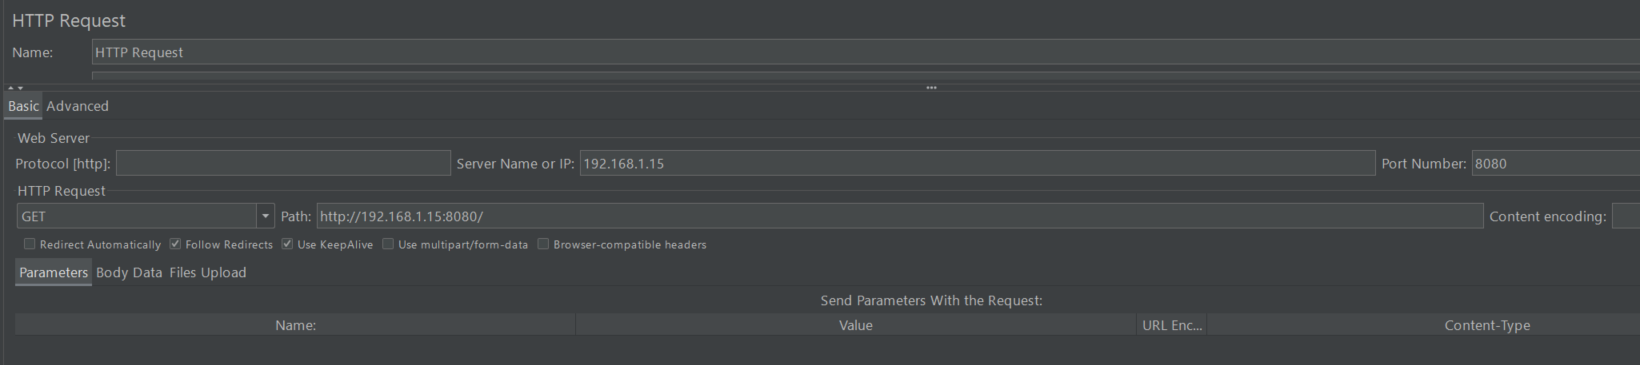
\includegraphics[scale=0.52]{images/configJmeter.png}
\caption[Configuración HTTP Request JMeter]{Configuración de las peticiones HTTP en Apache JMeter. Campos a tener en cuenta: Server name, Port Number, HTTP Request y Path.}%
\label{fig:JmeterConfig}
\end{figure}

En cuanto a la elección de los <<listeners>> se han seleccionado los siguientes debido a la utilidad de sus resultados:
\begin{itemize}
    \item View Results Tree: Nos ofrece cada una de las respuestas obtenidas de las peticiones HTTP, dentro de ellas podemos observar sus detalles.
    \item Agregate Report: Refleja una tabla con el resumen general del conjunto de las muestras obtenidas: Muestras, media, latencia, error, rendimiento... etc
    \item Response Time Graph: Devuelve un gráfico del tiempo de respuesta a lo largo del tiempo de muestreo
\end{itemize}
A mayores se ha instalado el pluging \textit{PerfMon} (Servers Performance Monitoring) que ofrece algunos gráficos más avanzados que pueden resultar interesantes, como los siguientes:

\begin{itemize}
    \item Active Threads Over Time: Gráfica que describe como los hilos han ido activándose a lo largo de la muestra. Proporciona una visión de como varía la carga de trabajo a lo largo del tiempo, lo que puede ayudar a identificar patrones de uso y momentos de mayor demanda en el sistema.
    \item Response Latencies Over Time: Esta gráfica analiza las latencias de respuesta obtenidas durante la ejecución de las pruebas. La latencia se refiere al tiempo transcurrido desde que se envía una solicitud hasta que se recibe la respuesta correspondiente. Este gráfico permite identificar los momentos en los que se producen retrasos en las respuestas del sistema y puede ayudar a detectar cuellos de botella o problemas de rendimiento.
    \item Bytes Throughput Over Time: Este gráfico muestra la cantidad de bytes transferidos en el sistema a lo largo del tiempo. Proporciona información sobre el rendimiento de la transferencia de datos en el sistema, lo que puede ser útil para evaluar la capacidad de la red o identificar problemas de ancho de banda.    
\end{itemize}

En la Figura~\ref{fig:listeners} se puede observar la lista de todos los listeners seleccionados.

\begin{figure}[h]
\centering
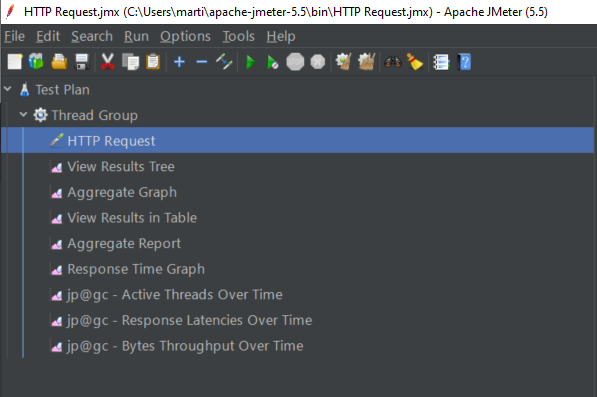
\includegraphics[scale=0.8]{images/listeners.png}
\caption[Listeners seleccionados]{Detalle de los tipos de clientes (\emph{Listeners}) utilizados en este escenario mediante Apache JMeter.}%
\label{fig:listeners}
\end{figure}

\subsection{Análisis de resultados}

A continuación, se mostrarán y analizaran los resultados obtenidos de las pruebas de carga realizadas sobre el servidor. Estos datos se mostrarán mediante las tablas y gráficas que ofrecen los propios listeners tras la finalización de las pruebas. 

\subsubsection{Escenario con 100 usuarios}


La Tabla~\ref{tab:100User} muestra los datos más interesantes del listener \textit{Agregate Report} obtenidos con la prueba que ha lanzado peticiones de 100 usuarios con un periodo de subida de 1 segundo (todos entran a la vez). Se trata de los tiempos de respuesta medidos en milisegundos por parte de la herramienta. Como puntos importantes de estos resultamos observamos que el error ha sido del 0\% y que las 100 peticiones se han resuelto en menos de 1 segundo, obteniendo así un rendimiento de 120 peticiones por segundo con un máximo de latencia de 90 milisegundos. En la Figura~\ref{fig:latencia100} puede observarse como este pico de latencia máximo aparece cuando al inicio de la prueba ya que es el momento en el que los 100 usuarios acceden al mismo tiempo, pero, a simple vista, puede verse que el servidor las resuelve de manera instantánea reduciendo la latencia a una media de 15 milisegundos hasta finalizar. 
En cuanto a la cantidad de Bytes recibidos y enviados, en la Figura~\ref{fig:respuestaJmeter} se puede observar cuál es la respuesta recibida por parte del servidor, se trata del texto plano que ofrece el servidor como bienvenida al acceder a su directorio raíz.\\

\begin{table}[h]
\begin{center}
\sffamily\small
\begin{tabular}{|c|c|c|c|c|c|c|c|}
\rowcolor{gray!20}
\hline
Muestras & Media & Mínimo & Máximo & \% Error & Rendimiento & KB/s Recibidos & KB/s enviados \\
\hline
100 & 26 & 6 & 90 & 0.00\% & 120.5/s & 42.71 & 14.35 \\
\hline
\end{tabular}
\caption[Salida <<Agregate Report>> con 100 hilos]{Datos obtenidos por el listener <<Agregate Report>> tras las pruebas realizadas con 100 usuarios y un tiempo de subida de 1 segundo, tiempos de respuesta en milisegundos}%
\label{tab:100User}
\end{center}
\end{table}


\begin{figure}[h]
\centering
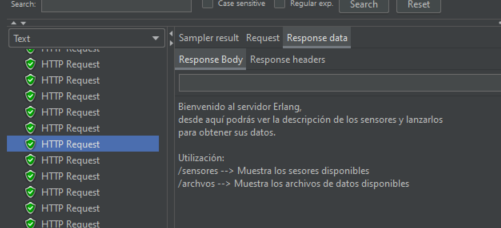
\includegraphics{images/respuestaJmeter.png}
\caption[Detalles de una HTTP Request obtenida]{Detalle de la respuesta obtenida por parte del servidor a todas las peticiones realizadas por la prueba de carga desde Apache JMeter.}%
\label{fig:respuestaJmeter}
\end{figure}


\begin{figure}[h]
\centering
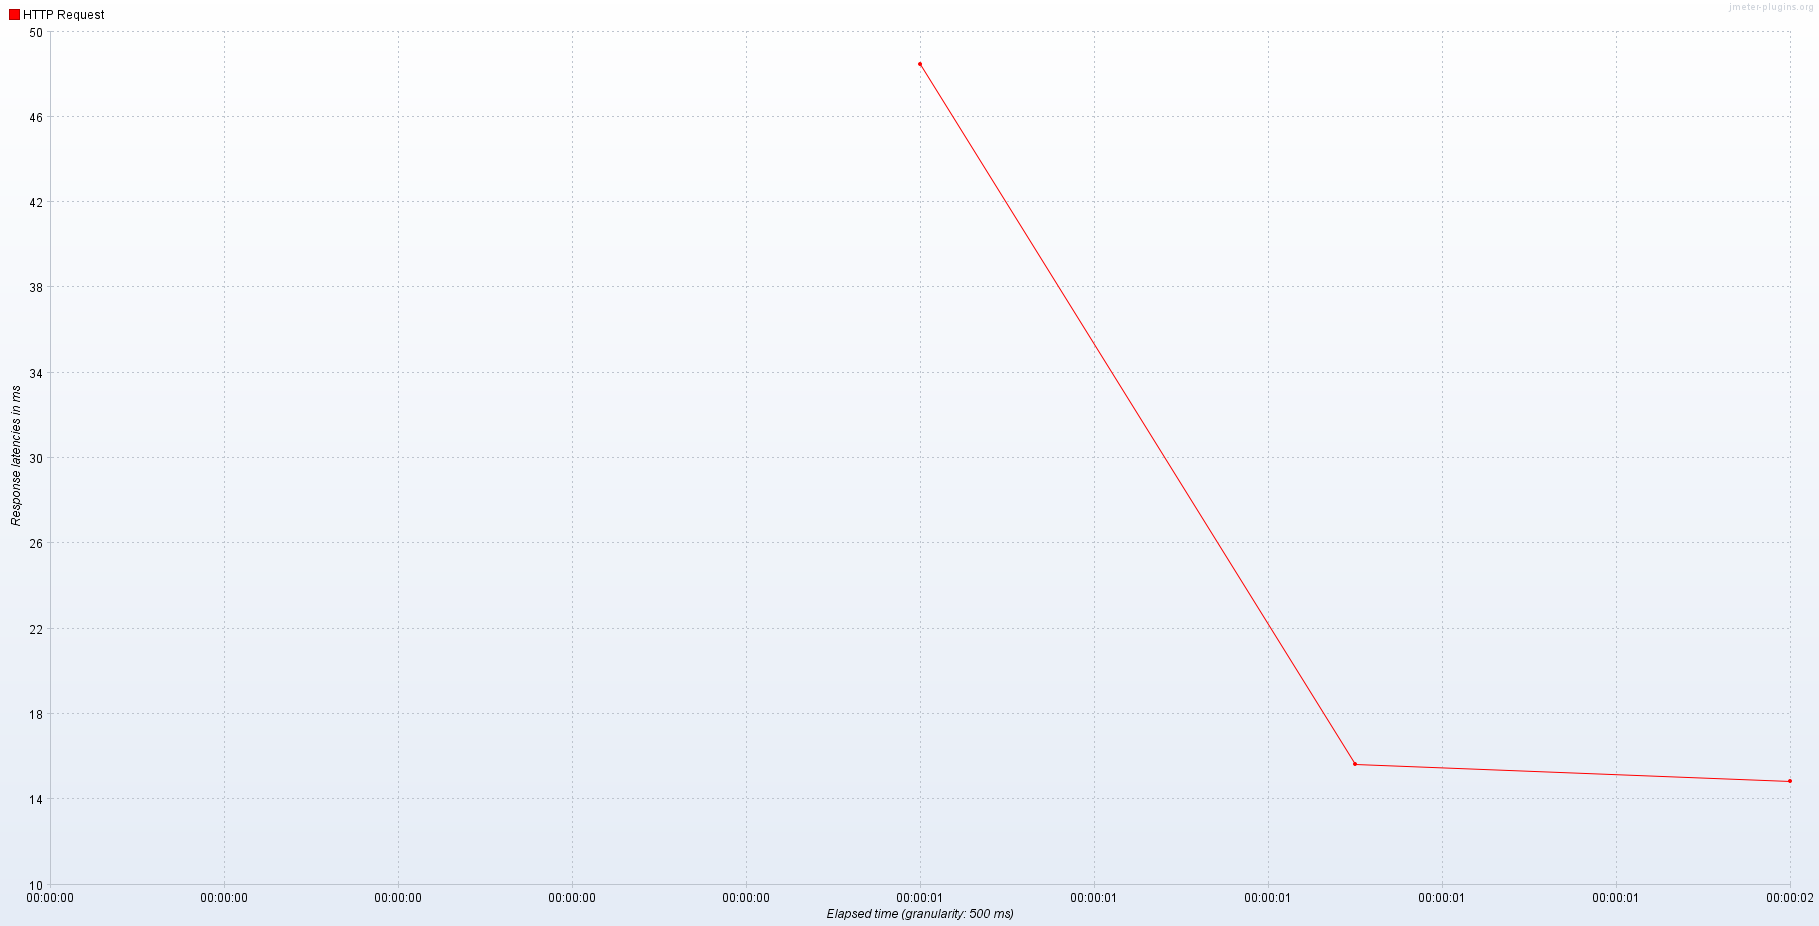
\includegraphics[scale=0.28]{images/latenciaGraf100.png}
\caption[Evolución de la latencia con 100 usuarios]{Evolución de la latencia en resolución de las peticiones desde 0 hasta 100 usuarios. Eje X medido en {\ttfamily hh:mm:ss} y eje Y medido en milisegundos.}%
\label{fig:latencia100}
\end{figure}



\subsubsection{Escenario con 15000 usuarios}

La Tabla~\ref{tab:15000User} muestra los datos más interesantes del listener \textit{Agregate Report} obtenidos con la prueba que ha lanzado peticiones de 15000 usuarios con un periodo de subida de 1 segundo (todos entran a la vez). Se trata de los tiempos de respuesta medidos en milisegundos por parte de la herramienta.

Como puntos importantes de estos resultamos observamos que se ha obtenido un error del 2,09\% por lo que en algún punto de la prueba se ha superado la cuota del servidor, para obtener más información sobre este fallo debe analizarse la salida obtenida por el terminal de ejecución el servidor representada en la Figura~\ref{fig:warning}, en ella aparece un Warning que se repite durante toda la prueba <<Ranch acceptor reducing accept rate: out of file descriptors>>, este aviso nos indica que el servidor ha llegado a su límite de descriptores, los descriptores de archivo son recursos limitados en un sistema operativo y se utilizan para representar archivos, sockets y otros objetos que pueden ser leídos o escritos. Cuando un servidor alcanza el límite de descriptores de archivo, no puede aceptar nuevas conexiones y, por lo tanto, reduce su tasa de aceptación, posteriormente veremos como solucionar esto en caso de necesitar tal capacidad de resolución de peticiones.

Por otro lado, el rendimiento del servidor ha sido muy alto, se han resuelto una media de 2318 peticiones por segundo lo cual indica una gran capacidad de resolución de peticiones simultáneas por parte de Cowboy. A continuación, analizaremos la gráfica obtenida de la evolución de la latencia a lo largo de la prueba.

En la Figura~\ref{fig:latencia15k} puede observarse como la latencia ha ido en aumento a lo largo del tiempo. Se ha dividido la gráfica en tres partes: 
\begin{itemize}
    \item \textbf{(1)}: En esta primera sección que abarca los dos primeros segundos de la prueba, la latencia ha ido subiendo progresivamente según han ido creándose los hilos.
    \item \textbf{(2)}: Del segundo 2 al 5 podemos ver un aumento más escalonado de la latencia, esto se debe a que se están resolviendo muchas de las peticiones entrantes pero al seguir entrando gran cantidad de ellas ocurren picos de latencia.
    \item \textbf{(3)}: A partir del segundo 6 el servidor se satura y el tiempo de respuesta aumenta de manera vertical hasta finalizar la prueba, provocando así ciertos errores. Es en este punto en el que aparecen los Warning comentados anteriormente indicando que la cuota de descriptores de archivo ha llegado a su límite.
\end{itemize}




\begin{table}[h]
\begin{center}
\begin{tabular}{|c|c|c|c|c|c|c|c|}
\rowcolor{gray!20}
\hline
Muestras & Media & Mínimo & Máximo & \% Error & Rendimiento & KB/s Recibidos & KB/s enviados \\
\hline
15000 & 369 & 4 & 3118 & 2.09\% & 2318.0/s & 920.01 & 270.39 \\
\hline
\end{tabular}
\caption[Datos de <<Agregate Report>> con 15000 usuarios]{Datos obtenidos por el listener <<Agregate Report>> tras las pruebas realizadas con 15000 usuarios y un tiempo de subida de 1 segundo, tiempos de respuesta en milisegundos}%
\label{tab:15000User}
\end{center}
\end{table}

\begin{figure}[h]
\centering
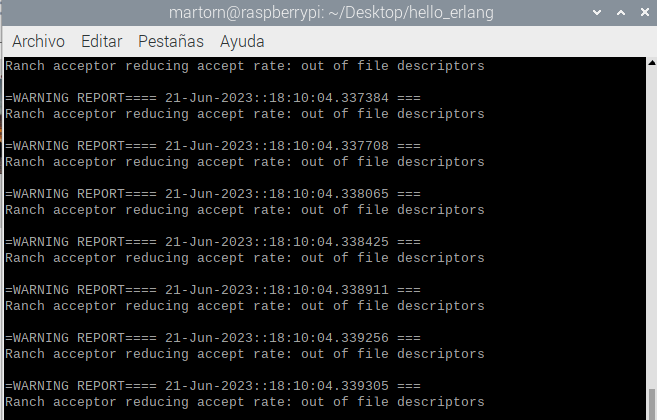
\includegraphics{images/warningServerDescriptors.png}
\caption[Warning del servidor por exceso de carga (15000 hilos)]{Warning obtenido en el terminal del servidor al someterlo a una carga de 15000 usuarios con un periodo de subida de 1, se observa el aviso de que no quedan descriptores de archivo.}%
\label{fig:warning}
\end{figure}


\begin{figure}[h]
\centering
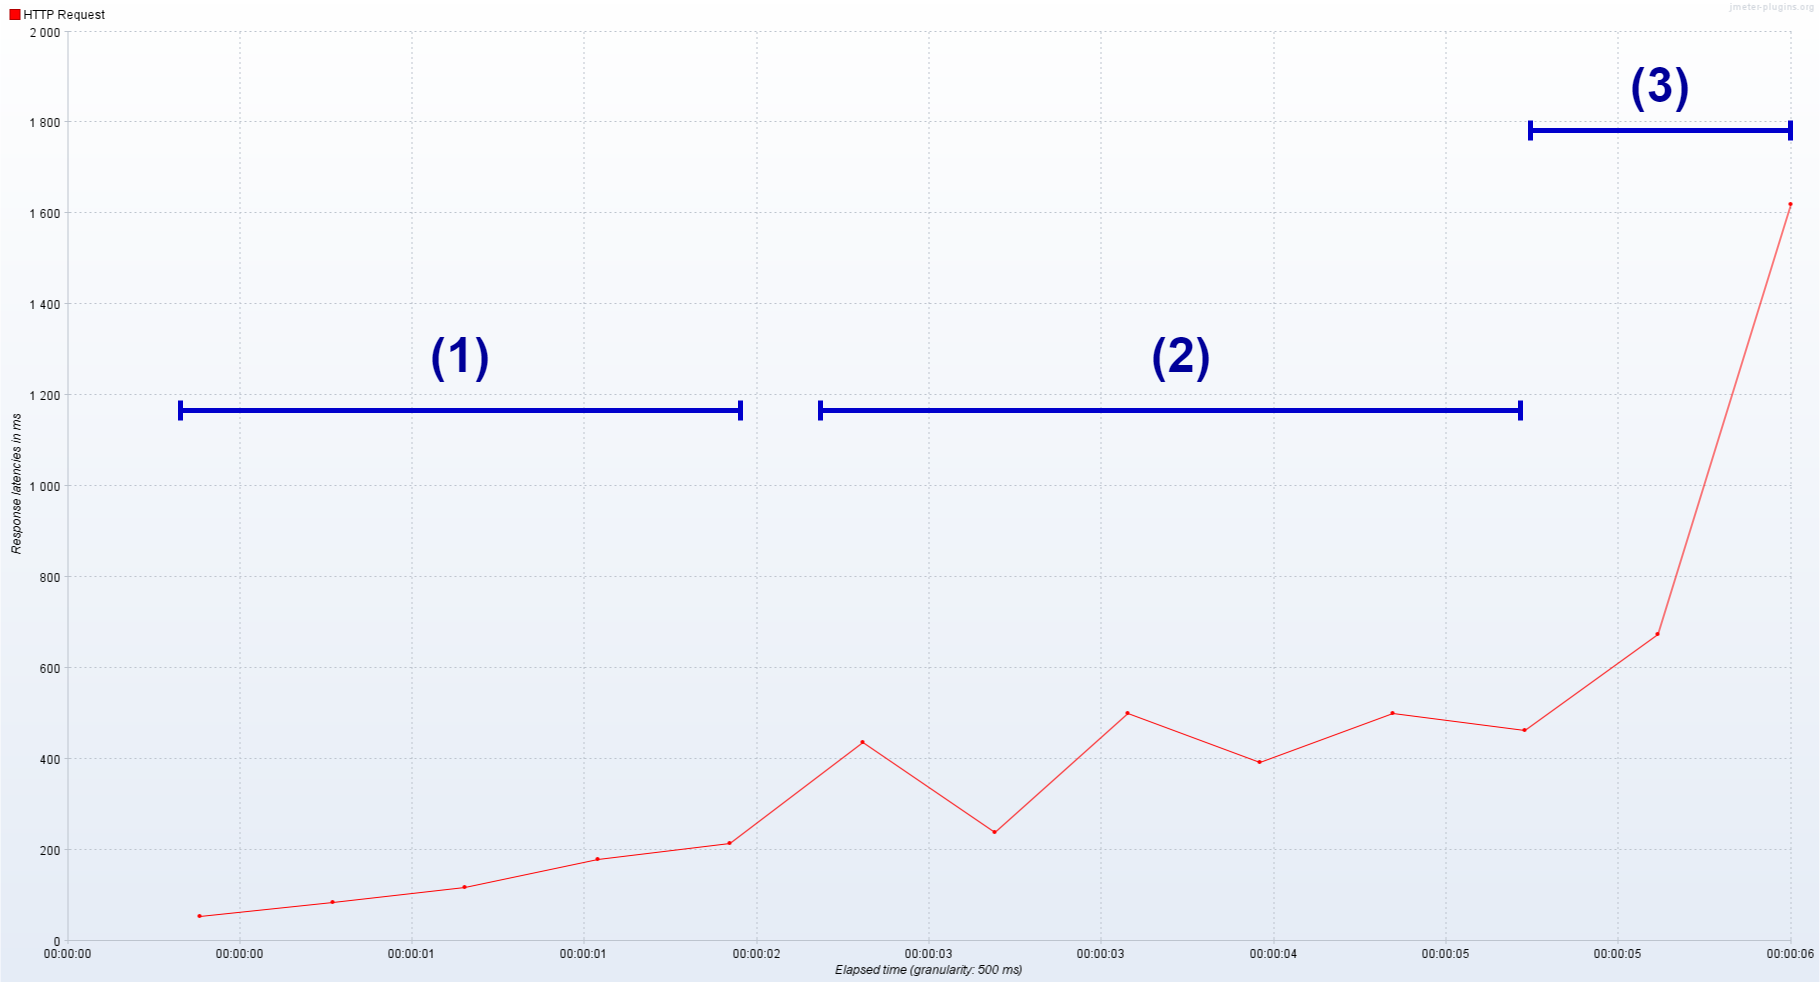
\includegraphics[scale=0.28]{images/latencia15k.png}
\caption[Evolución de la latencia con 15000 usuarios]{Evolución de la latencia en resolución de las peticiones desde 0 hasta 15000 usuarios. Eje X medido en {\ttfamily hh:mm:ss} y eje Y medido en milisegundos. La zona (1) delimita desde 0 hasta el segundo 2, zona (2) desde el 2 al segundo 5 y zona (3) del segundo 5 al final de la prueba.}%
\label{fig:latencia15k}
\end{figure}


La Tabla~\ref{tab:1500010sUser} muestra los datos más interesantes del listener \textit{Agregate Report} obtenidos con la prueba que ha lanzado peticiones de 15000 usuarios con un periodo de subida de 10 segundos. Se trata de los tiempos de respuesta medidos en milisegundos por parte de la herramienta.

A través de estos resultamos observamos que se ha obtenido un error del 0,00\% por lo que, a pesar de ser tal cantidad de usuarios (15000), al no acceder de manera simultánea sino a lo largo de 10 segundos, el servidor ha sido capaz de ir resolviendo las peticiones de manera constante sin saturarse obteniendo así un pico máximo de latencia de 148 ms y un rendimiento medio de 998.2 peticiones resueltas por segundo.

En la Figura~\ref{fig:latencia15k10s} puede observarse como la variación de la latencia ha sido constante a lo largo del tiempo dependiendo de la carga de usuarios y la revolución de peticiones a lo largo de la zona (1), entre el segundo 6 y el 7 aparece un pico algo más elevado, esto puede deberse a que en este momento la carga de peticiones sea muy elevada, al superar los 10 segundos el servidor empieza a estabilizar su tiempo de latencia y por último, al superar los 13 segundos zona (2) comienza el descenso debido a que la mayoría de peticiones ya han sido resueltas. Para poder asegurarnos de que esta teoría es correcta, podemos utilizar la Figura~\ref{fig:hilosactivos} que nos muestra los hilos activos a lo largo de la prueba, en esta gráfica observamos como, a partir del segundo 3 que encontramos el punto más elevado de hilos activos, con más de 180, estos comienzan a descender de manera escalonada hasta que, a partir del segundo 10 comienzan una bajada mucho más progresiva que se mantiene cerca de los 20 hilos activos hasta la finalización de la prueba. Estos datos indican que el servidor es capaz de resolver gran cantidad de peticiones siempre que no se supere el umbral de descriptores, de tal manera que, si la entrada de usuarios es paulatina y no simultánea, se obtienen unos rendimientos y una tasa de resolución de peticiones francamente buena. 




\begin{table}[h]
\begin{center}
\begin{tabular}{|c|c|c|c|c|c|c|c|}
\rowcolor{gray!20}
\hline
Muestras & Media & Mínimo & Máximo & \% Error & Rendimiento & KB/s Recibidos & KB/s enviados \\
\hline
15000 & 12 & 4 & 148 & 0.00\% & 998.2/s & 353.86 & 118.93 \\
\hline
\end{tabular}
\caption[Datos de <<Agregate Report>> con 15000 usuarios y 10 segundos de suboda]{Datos obtenidos por el listener <<Agregate Report>> tras las pruebas realizadas con 15000 usuarios y un tiempo de subida de 10 segundos, tiempos de respuesta en milisegundos}%
\label{tab:1500010sUser}
\end{center}
\end{table}

\begin{figure}[h]
\centering
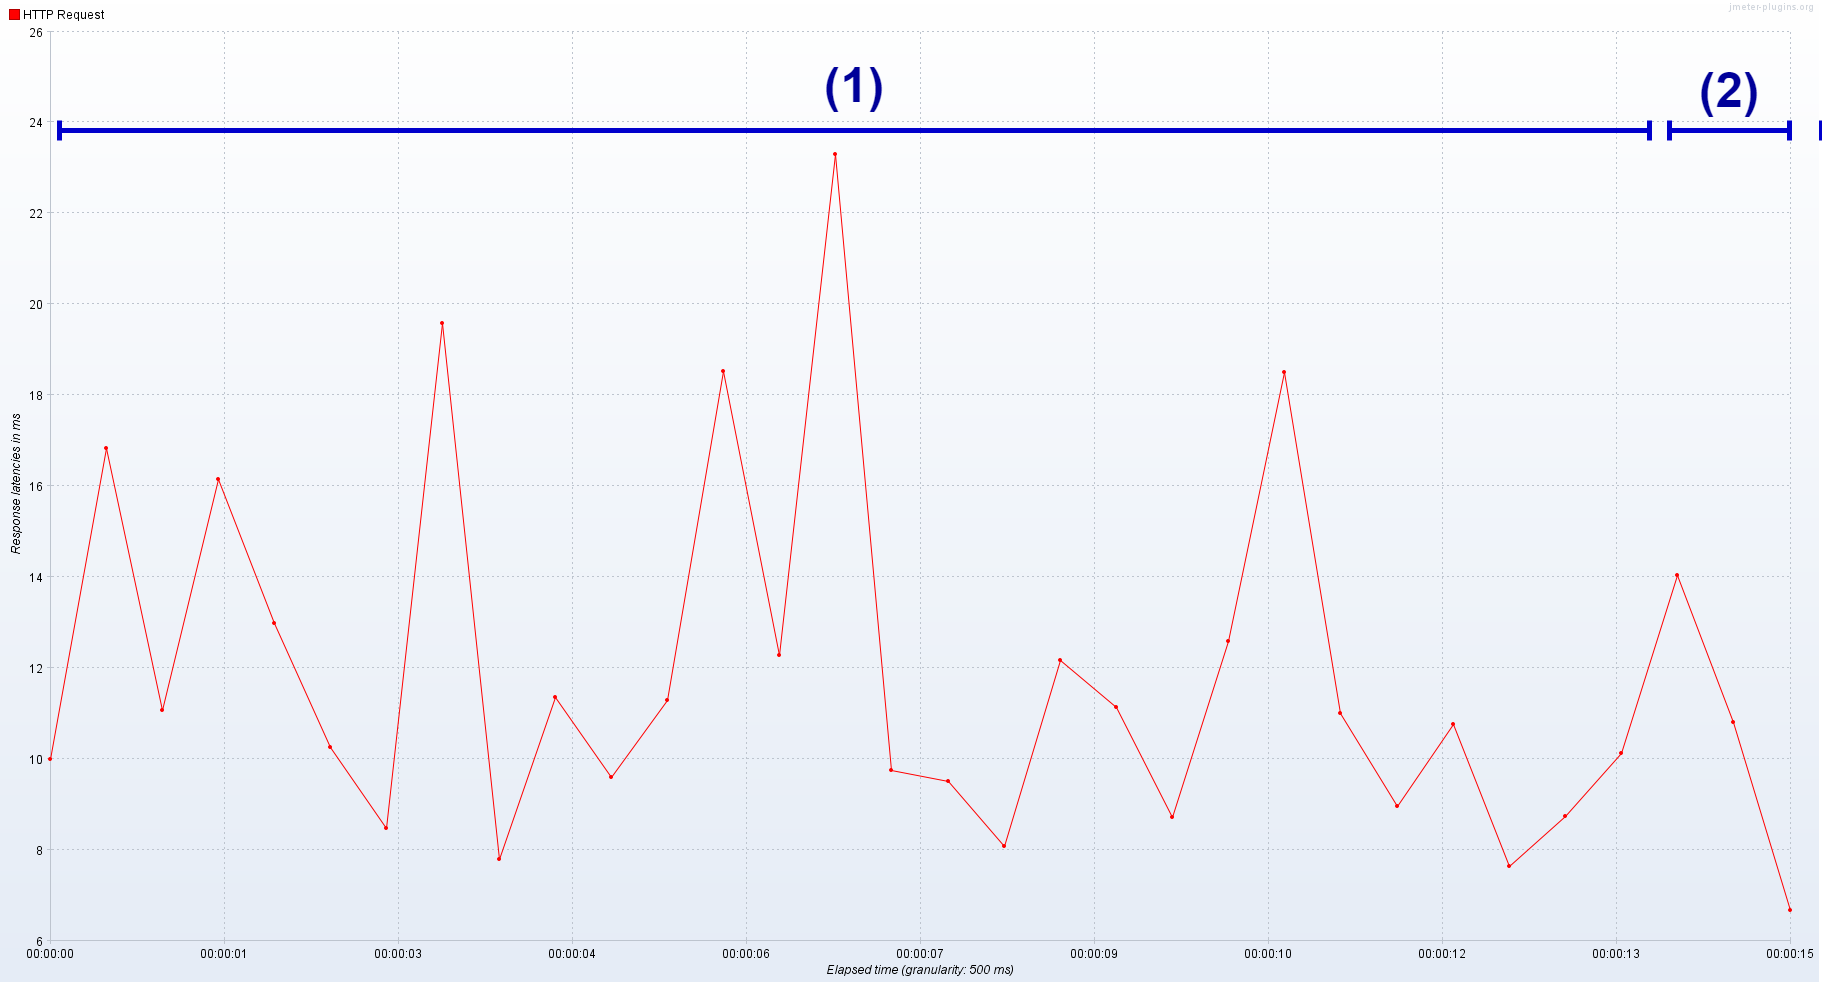
\includegraphics[scale=0.28]{images/latencia15k10s.png}
\caption[Evolución de la latencia con 15000 usuarios y 10 segundos de subida]{Evolución de la latencia en resolución de las peticiones desde 0 hasta 15000 usuarios con 10 segundos de periodo de subida. Eje X medido en {\ttfamily hh:mm:ss} y eje Y medido en milisegundos . La zona (1) delimita desde 0 hasta el segundo 14 y zona (2) desde el segundo 14 al final de la prueba.}%
\label{fig:latencia15k10s}
\end{figure}

\begin{figure}[h]
\centering
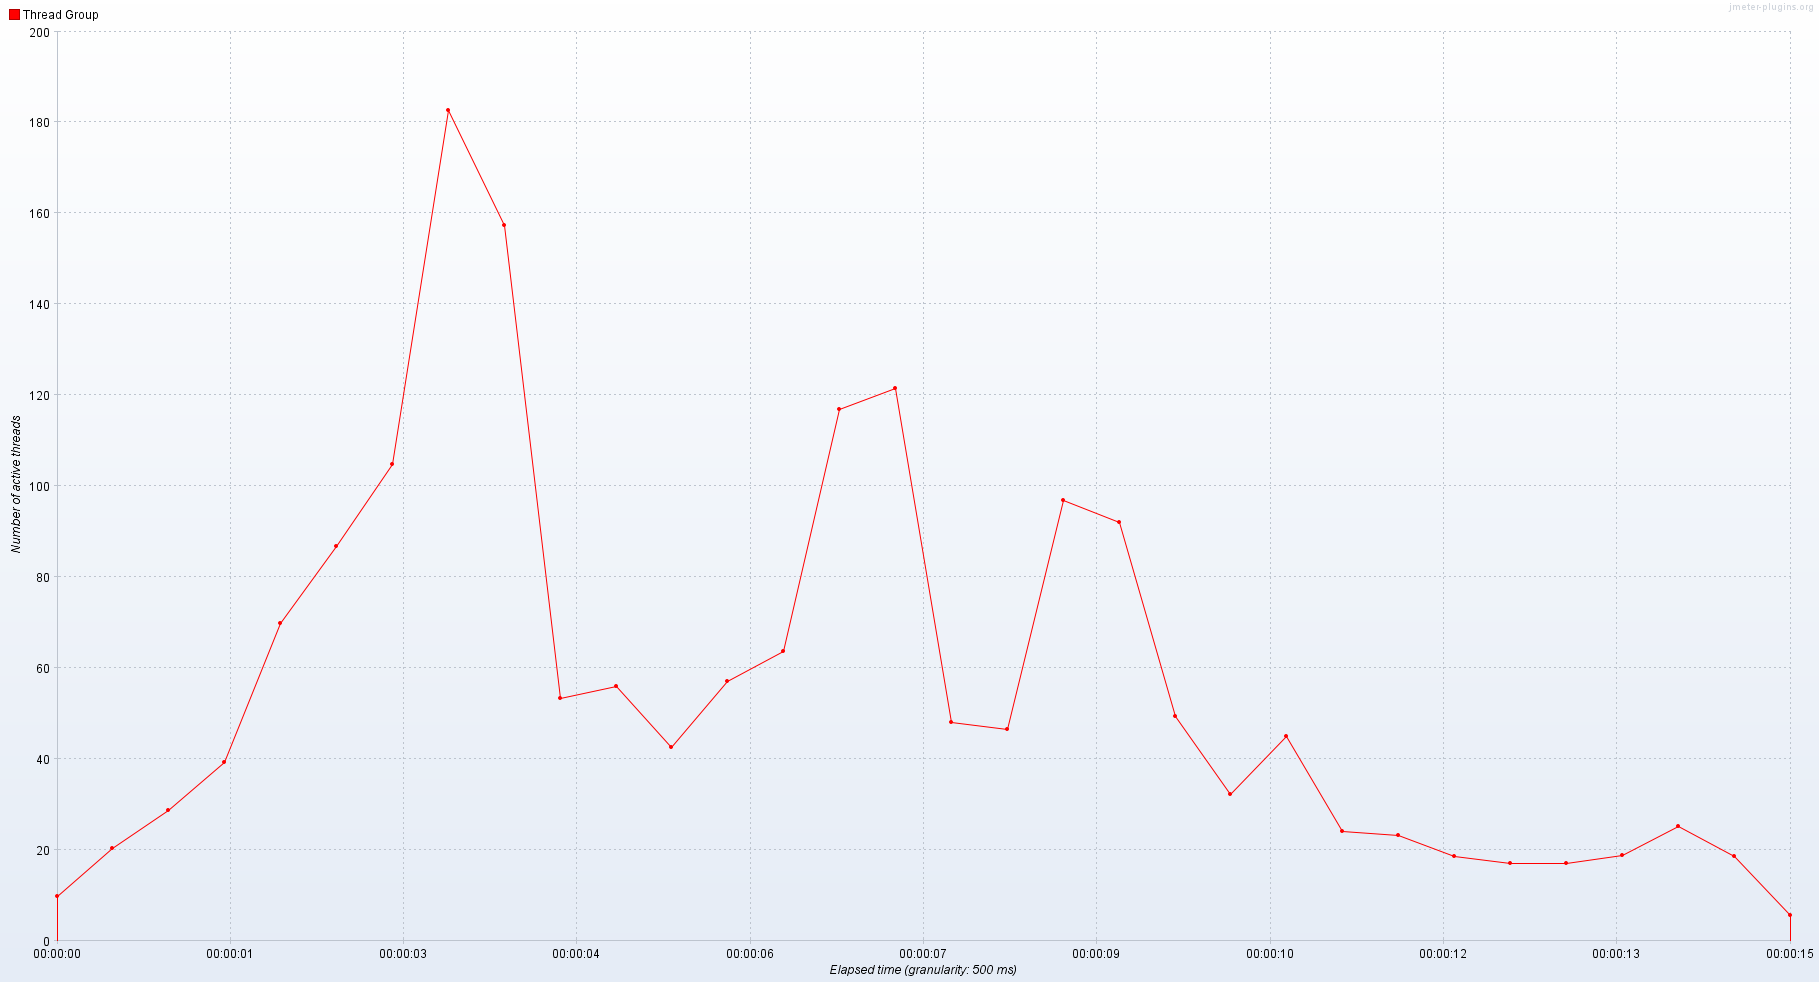
\includegraphics[scale=0.28]{images/hilosActivosGraf15k10subida.png}
\caption[Evolución de hilos activos con 15000 usuarios y 10 segundos de subida]{Evolución de los hilos activos en resolución de las peticiones desde 0 hasta 15000 usuarios con 10 segundos de periodo de subida. Eje X medido en {\ttfamily hh:mm:ss} y eje Y medido en número de hilos.}%
\label{fig:hilosactivos}
\end{figure}

\chapter{Conclusiones}

\section{Grado de consecución de los objetivos}

Los objetivos planteados en el Apartado\ref{sec:Objetivo} se han alcanzado totalmente. Tras varios meses de trabajo y dificultades, se ha logrado crear un servidor plenamente operativo utilizando lenguaje Erlang OTP que permite lanzar la lectura de ciertos sensores y visualizar los datos obtenidos por los mismos. Este servidor dispone de un manual de uso para que el usuario entienda sin dificultad el funcionamiento de la API REST creada y a su vez está pensado para que un administrador pueda crear más funcionalidad añadiendo o quitando sensores de manera sencilla.

Se ha conseguido un servidor usando Cowboy, que funciona de manera eficiente y con un rendimiento que sobrepasa las necesidades requeridas por parte del sistema y todo ello implementado sobre una Raspberry-Pi 3, por lo que se trata de un sistema portable y fácilmente implementable.

\section{Dificultades encontradas}

En el transcurso del proyecto han aparecido ciertos obstáculos que se han tenido que solventar, se han dividido en dos: problemas con los sensores y problemas con Erlang OTP.

En primer lugar, al comienzo del proyecto, tras la configuración de la placa R-Pi, surgieron problemas con la conexión del sensor MPU6050, el principal problema fue que la placa R-Pi no detectaba de manera correcta el sensor, se probaron sus dos tipos posibles de conexiones (SPI e I2C) y tras varios días de intentos fallidos se decidió descartar este sensor y se sustituyó por el sensor de ultrasonido HC-SR04. Este tipo de conexiones son sencillas y su uso es habitual por lo que no se contaba con tener este tipo de problemas.

Por otro lado, surgieron problemas de incompatibilidad entre los diferentes tipos de servidores posibles a implementar utilizando Erlang OTP sobre la placa R-Pi, esto ha ocurrido debido a que están pensados para ser ejecutados sobre Linux y algunas de las librerías de Raspbian están algo anticuadas o no son compatibles con las de Erlang, se probaron varias opciones de servidores y librerías y finalmente se decidió utilizar Cowboy por su fácil instalación y uso.

Finalmente, el lanzamiento de los sensores desde el servidor no fue fácil debido a los protocolos de seguridad que utiliza Cowboy sobre Erlang, la idea inicial era directamente lanzar el comando usando funciones Erlang como <<cmd>> pero los programas no eran lanzados correctamente ni los datos almacenados en el lugar esperado, es por ello que al final se ha usado Erlang ports para crear una conexión a través de un puerto desde el servidor a la placa R-Pi y de esta manera ejecutar código almacenado en la misma. Para almacenar los archivos en el lugar deseado simplemente se guardan en el servidor (el propio programa lo almacena ahí) y este lo puede leer de su propio directorio.


\section{Desviaciones sobre la planificación}

\subsection{Desviaciones temporales}
El trabajo se inició el día 20 de febrero de 2023 y su fecha final estimada era el 4 de julio. Finalmente con las dificultades encontradas y por otro lado los avances con respecto al tiempo estimado realizados en alguna de las actividades se ha finalizado el proyecto con 6 días de retraso. Este retraso no ha sido considerado un grave problema ya que se ha llegado a la fecha límite de entrega del trabajo y se han cumplido las tareas propuestas.
En la Figura~\ref{fig:gantReal} se muestra la diferencia entre el diagrama Gantt previsto y el Gantt real, con rojo marcado donde ha habido retrasos y verde donde se han realizado las tareas en menor tiempo del previsto.

\begin{figure}[h]
\centering
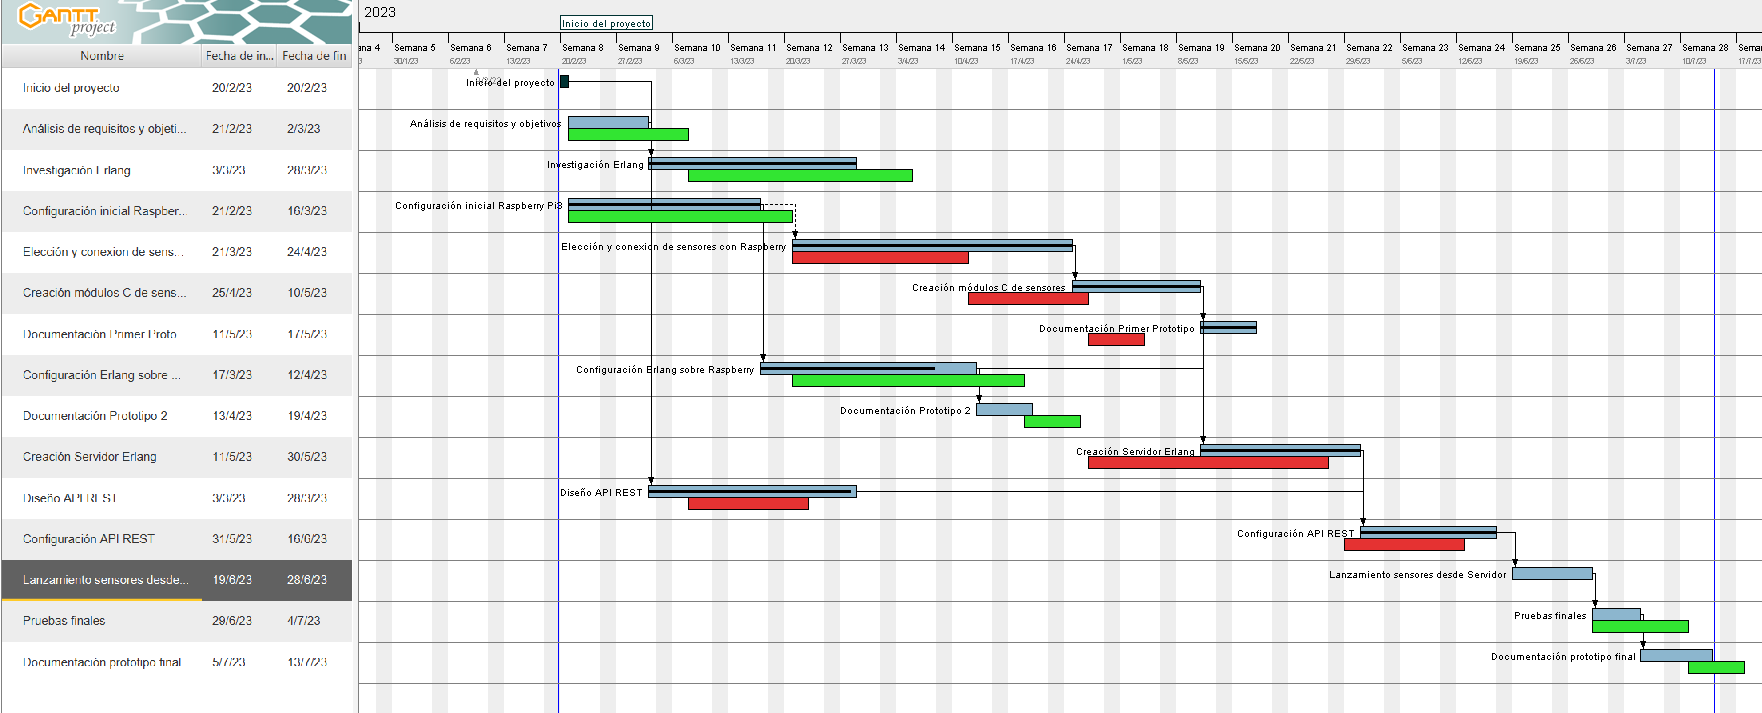
\includegraphics[scale=0.48]{images/gantProyectReal.png}
\caption[Diagrama de Gantt final]{Diagrama de Gantt real con avances y retraso (azul) frente al diagrama Gantt de la planificación inicial (rojo).}%
\label{fig:gantReal}
\end{figure}

\subsection{Desviaciones en presupuesto}

Una diferencia que si que ha sido notable con respecto a la planificación ha sido el número de horas necesarias para la realización del proyecto, debido a que el desarrollador disponía de pocos conocimientos sobre la materia (riesgo valorado en la Sección~\ref{sec:riesgos}) y los problemas comentados en el apartado anterior, el número de horas de trabajo ha aumentado en 120, lo que conlleva a un aumento del presupuesto total en concepto de recursos humanos. Este aumento ha sido de 2280\texteuro{} , por lo que el presupuesto ha pasado de los 6000\texteuro{}  estimados en el Apartado~\ref{sec:recHumanos} a 8280\texteuro{} .

Por último, el gasto en hardware final ha sido el que se observa en la Tabla~\ref{tab:hardwareFinal}, en ella aparecen las tiendas en las que se han adquirido los componentes y su precio específico, en comparación con lo estimado en la Sección~\ref{sec:recHardware} se ha reducido el coste en 41,71\texteuro{}.

\begin{table}[h!]
\begin{center}
\sffamily
\begin{tabular}{|l|c|c|r|}
\hline
\rowcolor{gray!20}
\textbf{Componente} & \textbf{Tienda} & \textbf{Cantidad}  & \textbf{Precio}  \\
\hline
Kit Raspberry-Pi 3 & Compass DHM projects & 1 & 68,93\officialeuro  \\
\hline
Sensor HMC5983 & Sensorae.com & 1 &  6,69\officialeuro \\
\hline
Sensor MPU6050 & Amazon.com & 1 &  3,49\officialeuro \\
\hline
Sensor HC-SR04 & PcComponentes.es & 1 &  2,68\officialeuro \\
\hline
Jumper Wire Cables & az-delivery.de & 3x40 pcs & 6,99\officialeuro \\
\hline
Resistencias 2.2K\(\Omega\) & Aliexpress.com & 10 pcs & 1,75\officialeuro \\
\hline
Resistencias 1K\(\Omega\) & Aliexpress.com & 10 pcs & 1,75\officialeuro \\
\hline
\rowcolor{gray!20}
\textbf{Total} & & & \textbf{85,29\officialeuro} \\
\hline
\end{tabular}
\caption[Costes definitivos componentes hardware]{Costes definitivos de Hardware utilizado para la realización del proyecto}%
\label{tab:hardwareFinal}
\end{center}
\end{table}

Tras el análisis de los costes reales al finalizar proyecto, se han obtenido diferencias en las horas de trabajo y en los costes hardware, por tanto, esto ha resultado un gasto final de 9360,29\texteuro{} en comparación con los 7122\texteuro{} estimados.

\section{Conocimientos aplicados y aprendizajes obtenidos}

A lo largo del desarrollo de este Trabajo de Fin de Grado se han puesto en práctica gran cantidad de conocimientos aprendidos en diferentes asignaturas, a continuación de enumera cada una de ellas junto con su aplicación en este proyecto:

\begin{itemize}
    \item \textbf{Interacción Persona Computadora}: Se ha utilizado para la gestión de sistemas que interaccionan con usuarios como es el caso del servidor, también para el uso de patrones y diseños fáciles de usar.
    \item \textbf{Sistemas Empotrados y Sistemas Digitales}: Conocimientos aplicados en todo aquello relacionado con la electrónica y el hardware.
    \item \textbf{Fundamentos de Programación}: Conocimientos básicos de programación, en este proyecto se ha utilizado lenguaje C, Python y Erlang OTP.
    \item \textbf{Evaluación de Sistemas Informáticos}: Utilizado para la creación de planes de prueba sobre el servidor para poner a prueba su rendimiento y funcionalidad.
    \item \textbf{Servicios y Sistemas Web junto con Diseño, Administración y Seguridad de Redes}: Para la creación y configuración del Servidor Web así como su interfaz y servicio API REST.
    \item \textbf{Diseño, Integración y Adaptación de Software y Fundamentos de Ingeniería de Software}: Para la planificación y análisis del proyecto mediante la creación de diagramas.    
\end{itemize}

A continuación, se detallan las competencias adquiridas o reforzadas a lo largo del proyecto:

\begin{itemize}
    \item Se ha aprendido a desarrollar un proyecto de este calibre, desde la planificación inicial hasta el análisis de requisitos, los planes de prueba, el análisis de riesgos y la documentación.
    \item Se ha aprendido lenguaje funcional Erlang OTP del que los conocimientos eran nulos, desde su instalación en una placa Raspberry-Pi hasta la creación de un servidor utilizando Cowboy.
    \item Se ha aprendido el funcionamiento de la placa R-Pi y de sus conexiones a hardware externo mediante los pines GPIO.
    \item Se han aumentado los conocimientos de programación en C y Python, especialmente en el uso de librerías para hardware externo como WiringPi.
    \item Se ha aprendido sobre protocolos de comunicación entre dispositivos, sus puertos y sus conexiones.
    \item Se ha descubierto el uso de SysML para la creación de diferentes diagramas que permiten el análisis y descripción de proyectos de estas características.
\end{itemize}

\section{Trabajo futuro}

El trabajo descrito en este documento está pensado para permitir a un administrador diversas ampliaciones futuras. El objetivo principal de cara al trabajo futuro era ofrecer un diseño del servidor sencillo y un manual de uso e instalación de las herramientas que permitiera a un administrador añadir o eliminar funcionalidad del sistema, sobretodo en el ámbito de los sensores. Las principales lineas a seguir son:

\begin{itemize}
    \item Crear una interfaz web más visual que permita al usuario moverse de manera más cómoda.
    \item Ampliar la cantidad de sensores, cada uno con una tarea diferente para poder monitorizar un sistema y que estos puedan ejecutarse de manera simultánea.
    \item Acceso a la información captada por los sensores en tiempo real, esto permitiría observar los datos de los sensores en directo para así tomar las medidas necesarias. Actualmente estos datos se leen y se almacenan en archivos que, tras la finalización de la lectura, son visualizables.
    \item Crear un prototipo portable compacto. Actualmente el prototipo físico se ha creado únicamente para pruebas con los sensores y no se ha diseñado un prototipo que sea resistente a golpes, humedad, transportable ni con conexiones sencillas como usb o tipo C para la conexión de los sensores.
    
\end{itemize}

\section{Conclusiones finales}

Tras la realización de este proyecto utilizando Erlang OTP como lenguaje principal, pueden obtenerse algunas conclusiones sobre este tipo de lenguaje para proyectos de estas características.

 Aunque Erlang OTP se desarrolló originalmente para aplicaciones de telecomunicaciones, también se ha utilizado con éxito en una amplia gama de otros dominios, incluyendo, como es el caso, servidores y sistemas embebidos como la Raspberry Pi. Se han descubierto grandes ventajas de este lenguaje a lo largo del proyecto, entre ellas:

 \begin{itemize}
     \item \textbf{La concurrencia}: Tras las pruebas realizadas con gran cantidad de usuarios se ha observado que un servidor sencillo como Cowboy implementado con Erlang, responde muy bien a grandes cantidades de hilos accediendo a la vez. Teniendo en cuenta que está siendo ejecutado sobre un sistema con limitaciones como lo es la Raspberry-Pi, denota un gran punto positivo para Erlang que el rendimiento sea tan bueno.
     \item \textbf{La tolerancia a fallos}: Una gran ventaja de la utilización de Erlang es que sus módulos implementan de manera interna una alta tolerancia a fallos. A lo largo de este proyecto, esta resolución de fallos se ha podido observar en diversas ocasiones y ha resultado muy útil en el marco de la creación de un Servidor Web.  Esto es especialmente importante en entornos donde la fiabilidad es crítica, como la recolección de datos de sensores. Si un sensor falla o se produce un error en el servidor, Erlang OTP permite manejar y recuperarse de manera controlada, evitando que el sistema se caiga por completo.
     \item \textbf{La mensajería y comunicación}:  Erlang OTP proporciona un modelo de programación basado en el intercambio de mensajes ligeros entre procesos. Esto es especialmente útil cuando necesitas comunicarte entre los diferentes componentes de tu sistema de recolección de datos, como en el caso de los sensores. Puede utilizarse este modelo de mensajes para coordinar la lectura de sensores, procesar los datos recibidos y enviar las respuestas a otros componentes del sistema.
    \item \textbf{La escalabilidad}: Los servidores basados en Erlang y especialmente Cowboy, están diseñados para escalar verticalmente y horizontalmente de manera efectiva. Esto significa se puede agregar más capacidad de procesamiento y recursos a medida que crece la cantidad de sensores o la carga de trabajo. La Raspberry Pi tiene recursos limitados en comparación con servidores más potentes, pero Erlang/OTP te permite aprovechar al máximo los recursos disponibles y escalar el sistema de manera eficiente.
 \end{itemize}

Por otro lado, también se han encontrado desventajas en el uso de Erlang, a continuación se describen las más importantes:

\begin{itemize}
    \item \textbf{Gran curva de aprendizaje}: Erlang/OTP sigue un paradigma de programación funcional, que puede diferir significativamente de los enfoques más comunes de programación imperativa o orientada a objetos vistos a lo largo de la carrera, lo que conlleva a que puede haber una curva de aprendizaje pronunciada para los desarrolladores que no están familiarizados con el lenguaje y las convenciones de Erlang/OTP, como ha sido el caso. Esto puede requerir tiempo y esfuerzo adicional para comprender y aprovechar al máximo la plataforma y un cambio de mentalidad y ajuste en la forma de abordar el diseño y la implementación del sistema.
    \item \textbf{Baja disponibilidad de bibliotecas y herramientas}: Aunque Erlang/OTP cuenta con una sólida biblioteca estándar, puede haber limitaciones en cuanto a la disponibilidad de bibliotecas y herramientas de terceros en comparación con otros lenguajes y plataformas más populares. Esto puede dificultar la integración con determinados componentes o servicios externos que podrían ser necesarios en el proyecto. Para ciertos componentes, sobretodo hardware externo utilizado en Raspberry-Pi, existe mucha información con el uso de Python, pero Erlang no es tan utilizado y esto lleva a que las búsquedas sean mucho más tediosas.
    
    \item \textbf{Menor comunidad y soporte}: Aunque Erlang/OTP cuenta con una comunidad activa de desarrolladores, su tamaño y alcance son más limitados en comparación con otros lenguajes y plataformas más populares, esto se observa de manera muy habitual cuando vamos a realizar una búsqueda sobre cuestiones específicas del sistema, en otros lenguajes existen muchos casos de fallos comunes o foros de preguntas y respuestas pero en el caso de Erlang es mucho más limitado y muchas veces anticuado. Esto podría resultar en una disponibilidad reducida de recursos de aprendizaje, documentación y soporte en línea, lo que podría dificultar la resolución de problemas o la obtención de ayuda en momentos críticos.
    
\end{itemize}

\appendix

\chapter{Contenido Digital}
\section{Contenido del repositorio}

Todo el código de este proyecto ha sido almacenado en la cuenta personal del alumno en Github de manera pública. En este repositorio se puede encontrar:\\

\dirtree{%
.1 HCSR04. 
.2 distance\_sensor.py: Código Python del sensor HC-SR04.
.2 ultrasonido.c: Código C del sensor HC-SR04. 
.1 HMC5983.
.2 i2c.py: Código Python del sensor HMC5983.
.2 cabeceoArchivo.c: Código C del sensor HMC5983.
.1 cowboyServer.
.2 sensorData: Almacena los datos obtenidos por los sensores.
.3 angulosCabeceo.txt: Datos del sensor HMC5983.
.3 distancias.txt: Datos del sensor HC-SR04.
.2 text: Almacena los JSON descriptores de sensores.
.3 inicio.json.
.3 magnetometro.json.
.3 sensores.json.
.3 ultrasonido.json.
.2 data\_handler.erl.
.2 hello\_erlang\_app.erl.
.2 hello\_erlang\_sup.erl.
.2 hello\_handler.erl.
.2 launch\_handler.erl.
.2 not\_found\_hanlder.erl.
.2 update\_handler.erl.
.1 TFG\_Martin\_Tornero.zip: Documentación del proyecto.
.1 README.md: manual de uso e instalación.
}

\section{Manual de instalación}

En las carpetas de los sensores encontramos dos archivos: Programa en C y programa en Python. El utilizado por el servidor es el programa en C. Para ejecutar los programas en C estos deben compilarse utilizando sus librerías. 

\begin{itemize}
    \item En el caso del sensor de ultrasonido HC-SR04 debe compilarse la librería WiringPi.h de la siguiente manera:
    \begin{lstlisting}[style=terminal]
    gcc -o ultrasonido ultrasonido.c -lwiringPi
    \end{lstlisting}
    
    \item En el caso del sensor magnetómetro HMC5983 debe compilarse la librería pigpio.h mediante el comando: 
     \begin{lstlisting}[style=terminal]
    gcc -o cabeceoArchivo cabeceoArchivo.c -lpigpio -lm
    \end{lstlisting}
    
\end{itemize}

Para lanzar el servidor debe disponerse de Erlang instalado y Cowboy configurado correctamente, para ello se recomienda seguir los pasos de la Sección~\ref{sec:ConfigCowboy}. Una vez completada la configuración inicial se pueden descargar los archivos de este repositorio accediendo a la URL \url{https://github.com/martorn/TFGMartinTorneroVazquez.git} o escaneando el código QR disponible en la Figura~\ref{fig:QR}.

\begin{figure}[h]
\centering

\includegraphics[scale=0.48]{images/qr.png}
\caption{Código QR del repositorio GitHub}%
\label{fig:QR}
\end{figure}
    

Por defecto, el servidor es lanzado en localhost sobre el puerto 8080, en caso de querer modificar esto podemos hacerlo de manera sencilla en hello\_erlang\_app.erl en su sección correspondiente. Por otro lado, es posible que surjan errores a la hora de lanzar los códigos de los sensores, es importante que se hayan compilado con anterioridad e indicar al servidor el lugar de almacenamiento del ejecutable del archivo y la localización de los archivos creados que almacenan los datos de los sensores. Estas modificaciones deben realizarse sobre el archivo launch\_handler.erl en sus funciones correspondientes.

Finalmente, si los pasos se han realizado correctamente, podemos lanzar el servidor ejecutando <<make run>> y acceder al mismo usando curl o a través de un navegador.

Los datos del repositorio han sido actualizados en Julio de 2023.



\newpage

\addcontentsline{toc}{chapter}{Referencias bibliográficas}
\bibliographystyle{ieeetr}
\bibliography{bibliografia} 

\end{document}